\documentclass[]{article}

\usepackage[english]{babel}
\usepackage[utf8x]{inputenc}
\usepackage[T1]{fontenc}

\usepackage[a4paper,margin=2 cm]{geometry}

%% Useful packages
\usepackage{amsmath}
\usepackage{graphicx}
\usepackage{para list}
\usepackage{indentfirst}
\usepackage{booktabs}
\usepackage{multirow}
\usepackage{clrscode}

\begin{document}
\title{Baseline Experiments on CIFAR-10 and CIFAR-100}
\author{Yufeng Cai - s1626868}
\maketitle
\section{Introduction}
CIFAR-10 and CIFAR-100 are well-known datasets for object recognition in images. CIFAR-10 comprises 60,000 colour images (3x32x32 pixels), with 10 object classes and it has been split into a training set of 40,000 images, a validation set of 10,000 images and a test set of 10,000 images. CIFAR-100 is similar to CIFAR-10, but has 100 classes; the training set size is again 40,000 images with validation and test sets each containing 10,000 images.

This report is about the baseline experiments of feed-forward neural network on CIFAR-10 and CIFAR-100. The experiments will focus on four aspects of neural network: \textbf{different network architectures, different activation function, normalisation and regularisation}. To investigate how these factors influence the recognition results, this report will set CIFAR-10 as an experimental test dataset and extend the results to CIFAR-100 dataset to see the performance.
\section{Network Architectures}
\subsection{Research Question}
According to J.Ba(2014), there are several reasons to indicate that deep neural network is better than shallow neural network:
\begin{enumerate}[ a)]
\item The deep net has more parameters; 
\item The deep net can learn more complex functions given the same number of parameters; 
\item The deep net has better inductive bias and thus learns more interesting/useful functions;
\item Current learning algorithms and regularization methods work better with deep architectures than shallow architectures; 
\end{enumerate}

Generally, a deeper net could give better recognition result although it will cost a lot on training process (eg. spend more time on updating parameters). Thus,  the balance between the accuracy and computational cost would be another aspect to investigate. In this section, based on one NN structure, we will extend more different structures to see how much will a deeper or wider architecture influence the recognition result and also to discover what problems exist in deeper or wider networks.

\textbf{Research question 1:} Does deeper and wider NN architectures provide better results?

\textbf{Research question 2:} Is there any problem exists in deep neural networks?
\subsection{Method}
To change the architecture of neural networks, we need to modify $num\_hidden$ variable and add a new hidden layer to tensor flow graphics. The code to add another layer is:

\emph{with tf.name\_scope('fc-layer-2'):} 

\emph{\qquad hidden\_2= fully\_connected\_layer(hidden\_1, num\_hidden, num\_hidden)}

The experiment design and some basic results are included in Table 1. We did 8 experiments with different NN architectures on both CIFAR-10 and CIFAR-100. First experiment is a baseline NN structure which provides a comparable result. The other experiments are the extended architecture based on the baseline experiment. We use $AdamOptimizer$ and set learning rate to $0.0001$ and $\epsilon = 0.001$. Also, to evaluate the training time, we record the training time for each epoch and calculate the average training time in the end. By comparing the performance of these experiments, we could investigate the influence of different depths and widths of NN architectures.
 
\begin{table}[ht]
\centering 
\caption{Experiment Design for Different Network Architectures}
\begin{tabular}{c c c c c c}
\toprule
No. & Method & Unit type & Architecture & Final Acc.(\%)(CIFAR-10) & Final Acc.(\%)(CIFAR-100) \\
\midrule
1 & NN & ReLU & 1 layer, 200 units & 51.93 & 22.17 \\
2 & NN & ReLU & 1 layer, 500 units & 51.86 & 23.86  \\
3 & NN & ReLU & 2 layer, 600 units & 51.90 & 23.96  \\
4 & NN & ReLU & 3 layer, 600 units & 51.87 & 23.21  \\
5 & NN & ReLU & 3 layer, 1500 units & 53.89 & 25.15  \\
6 & NN & ReLU & 3 layer, 3000 units & 53.68 & 24.90 \\
7 & NN & ReLU & 5 layer, 2500 units & 51.08 & 24.12  \\
8 & NN & ReLU & 5 layer, 5000 units & 52.11 & 24.08  \\
\bottomrule
\end{tabular}
\end{table} 

\subsection{Results and Discussion}
The plots of the evolution of training and validation process are shown below:

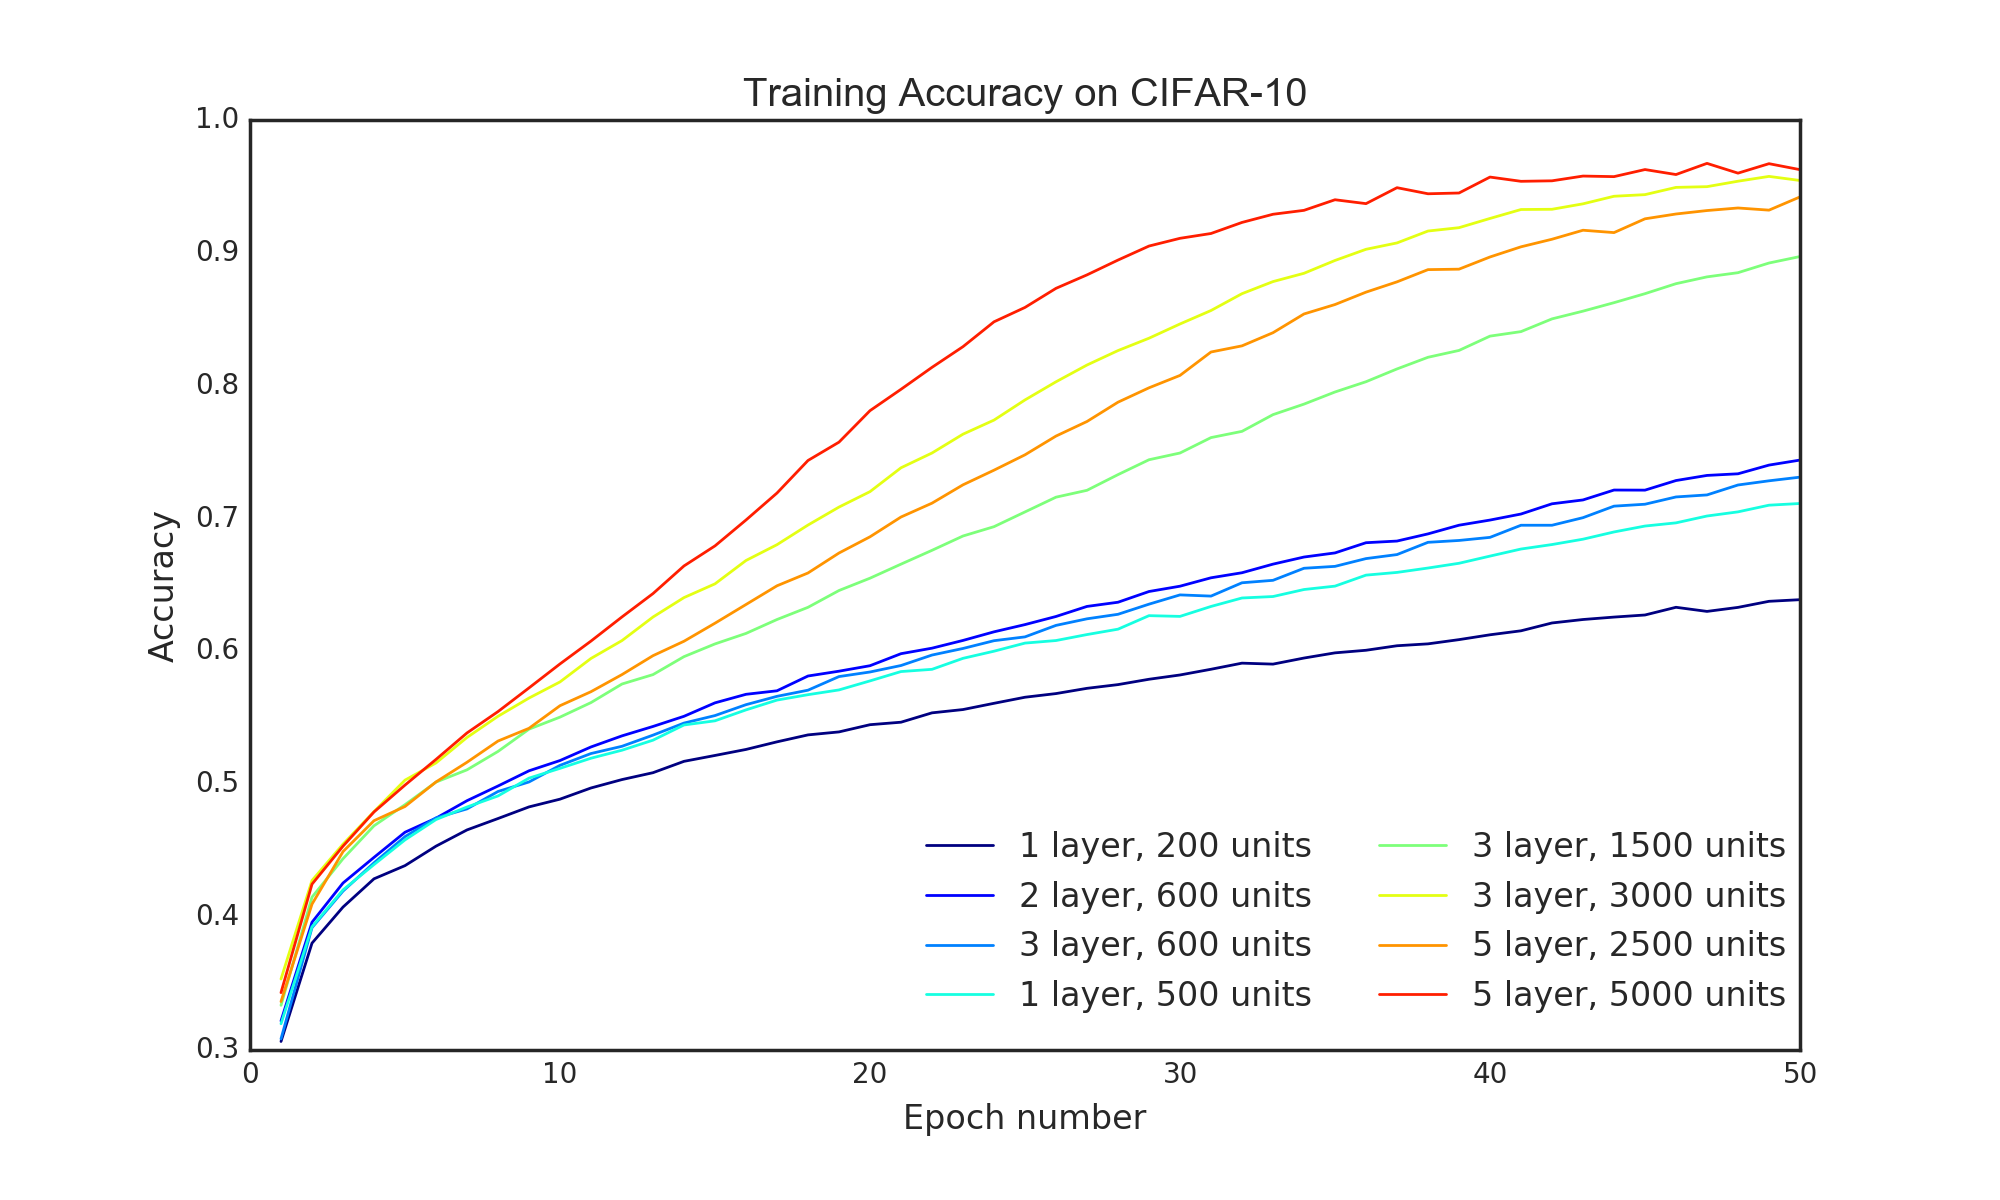
\includegraphics[width=3in]{NN_architures_train_acc}
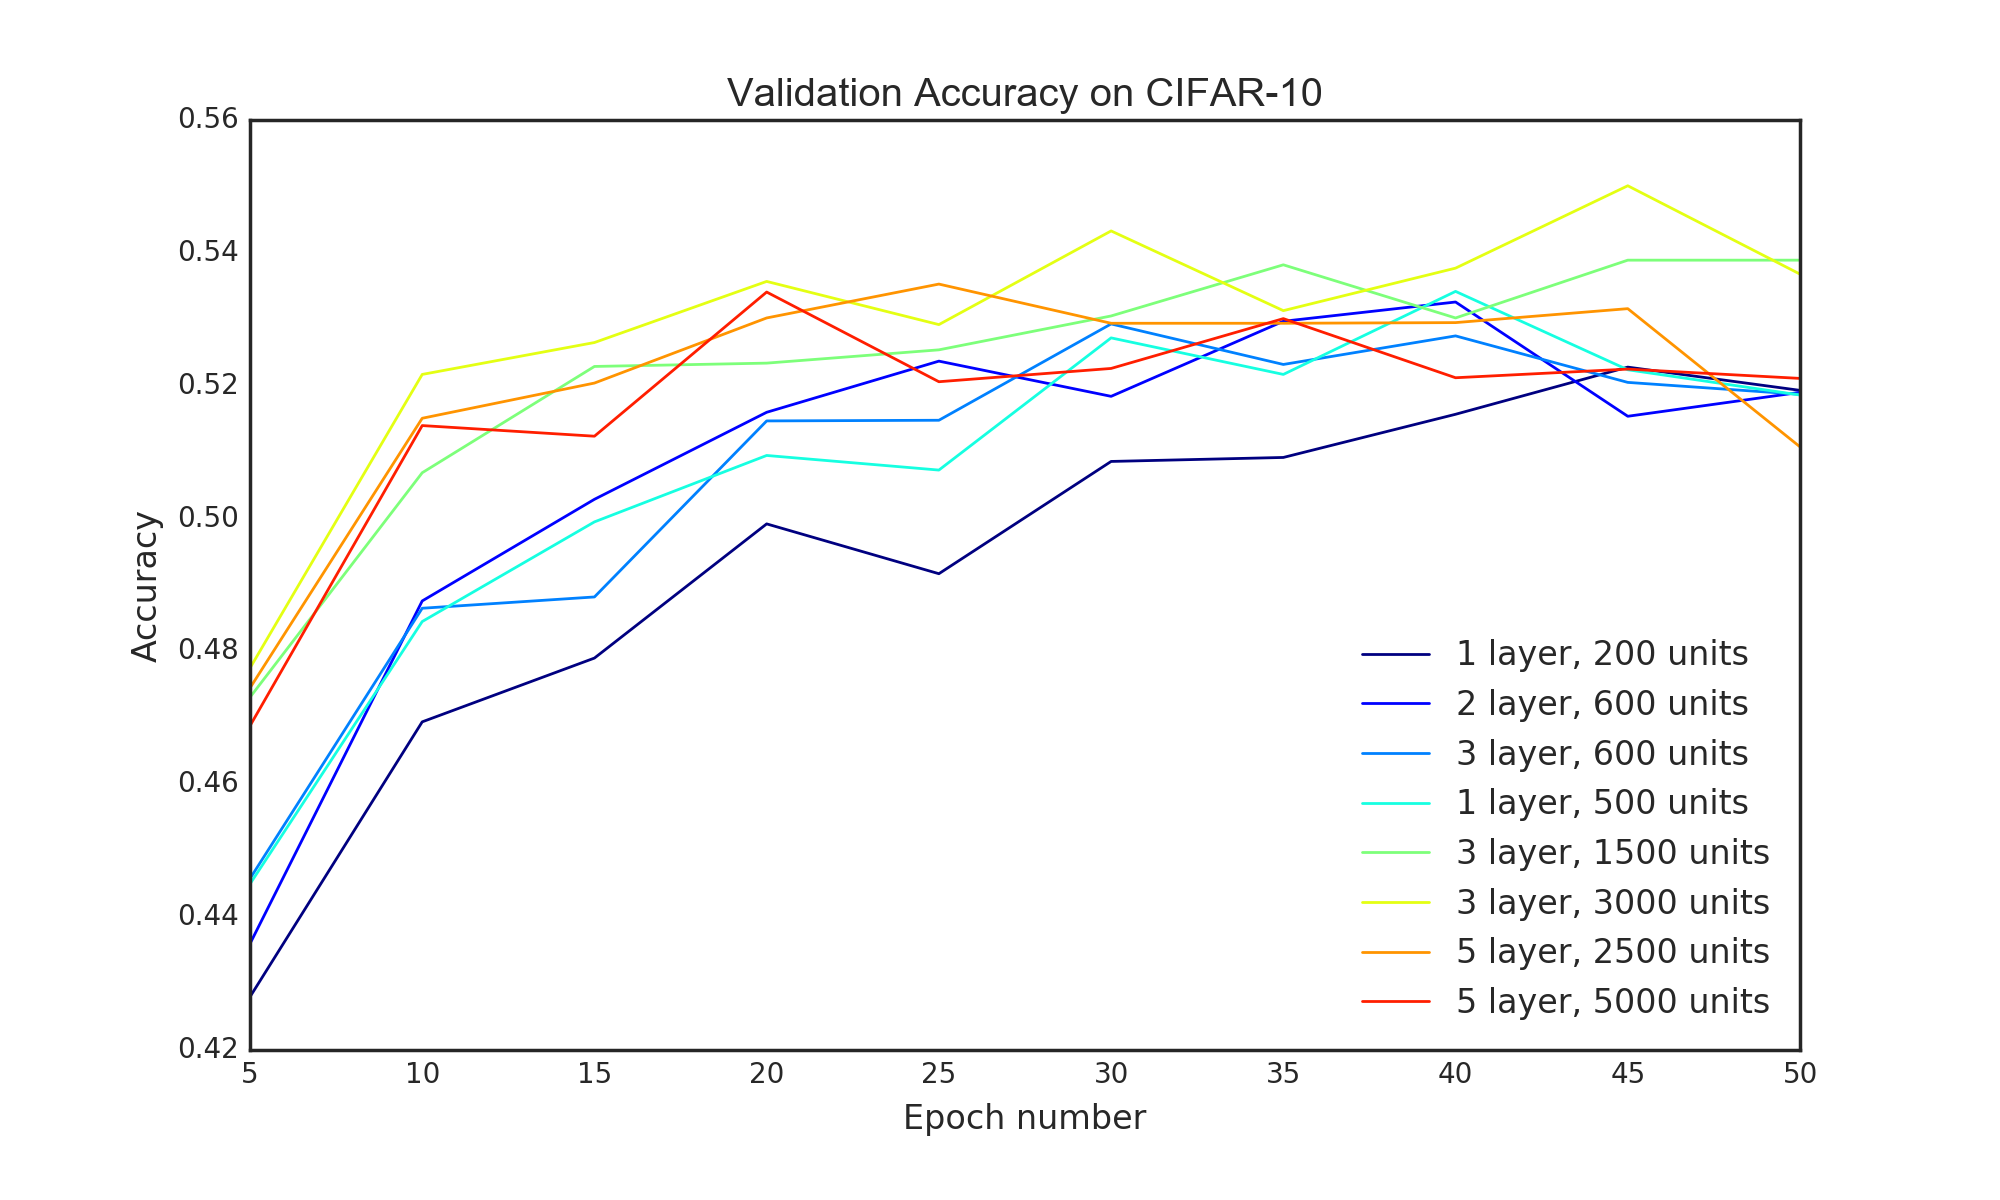
\includegraphics[width=3in]{NN_architures_valid_acc}

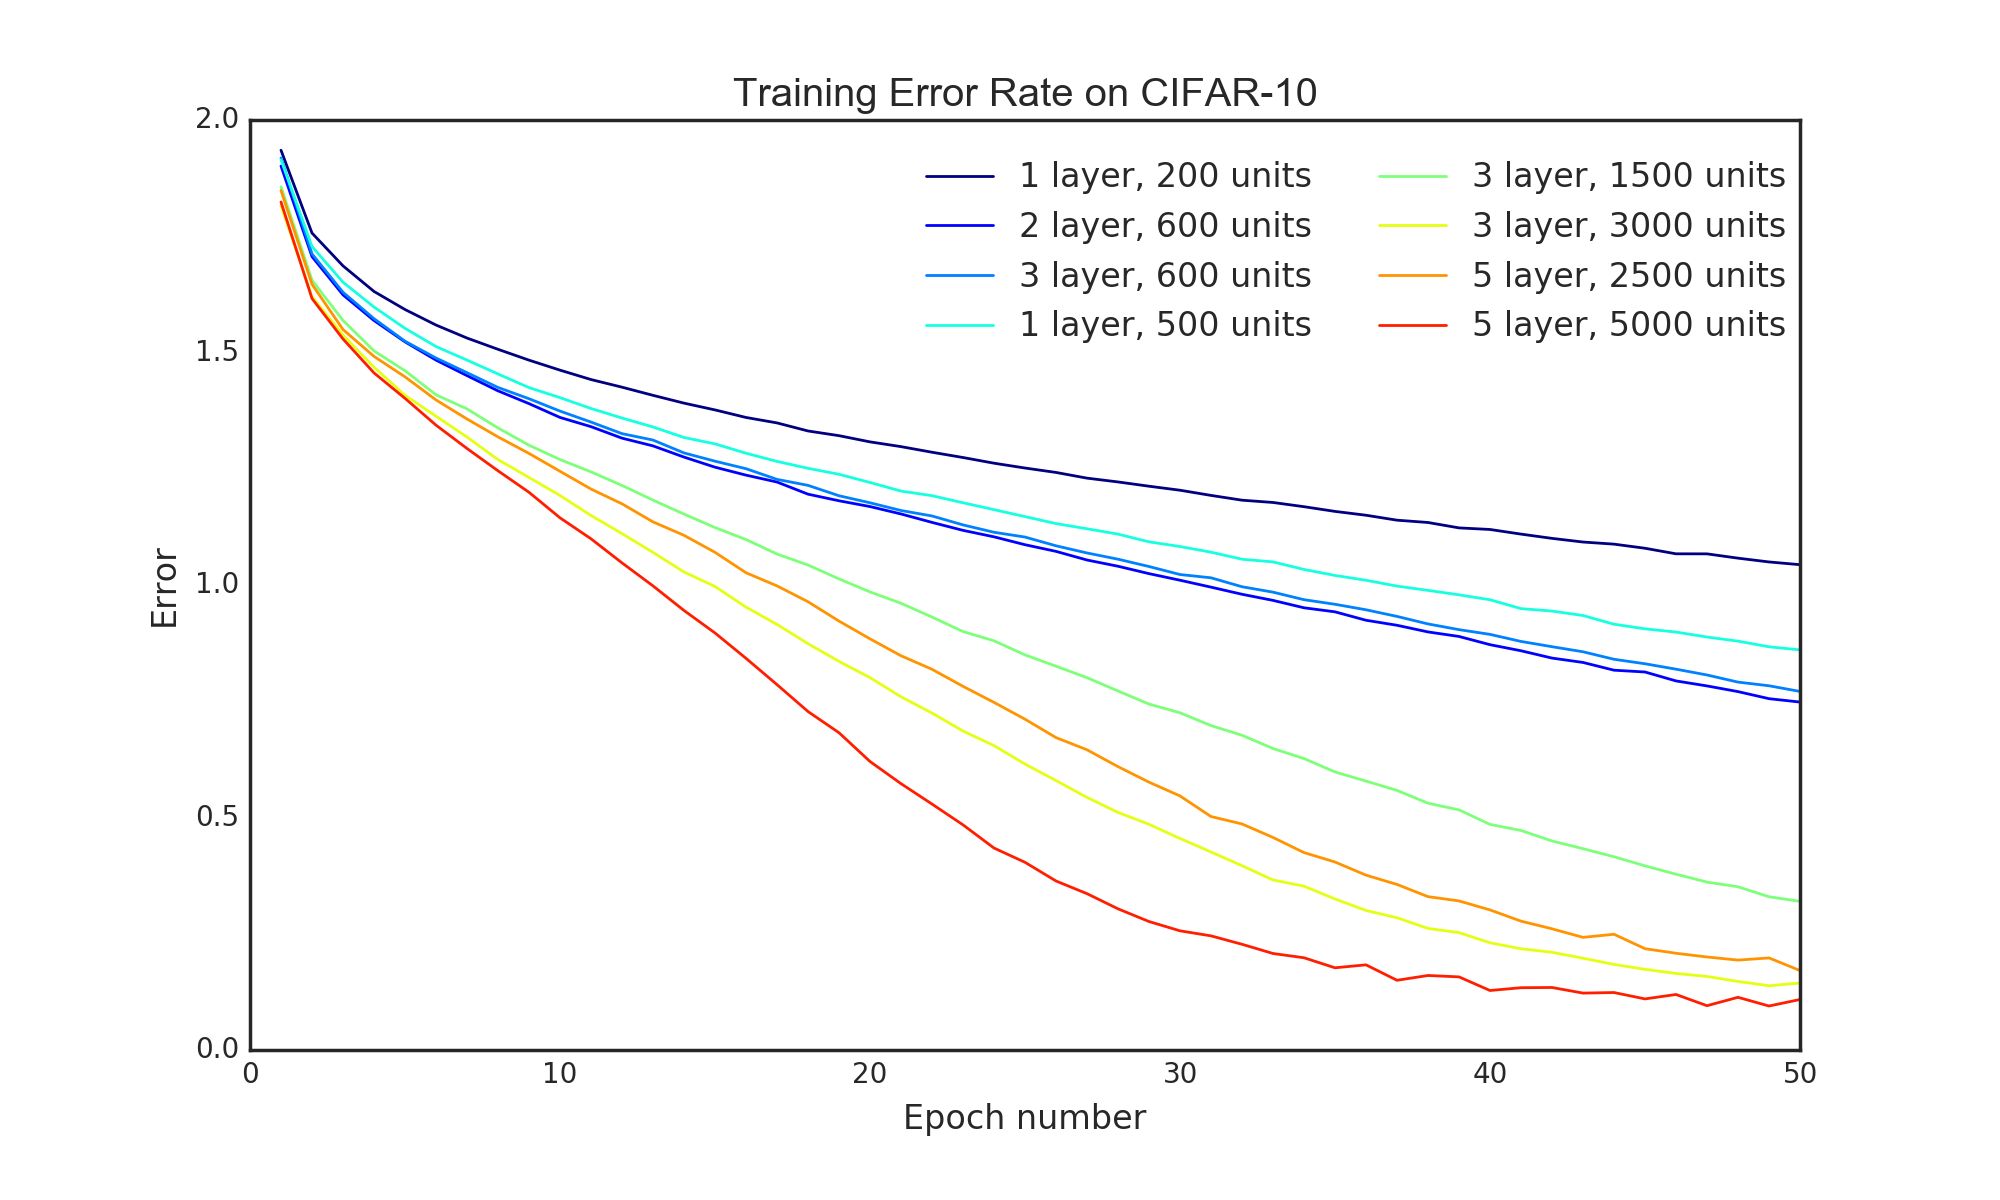
\includegraphics[width=3in]{NN_architures_train_err}
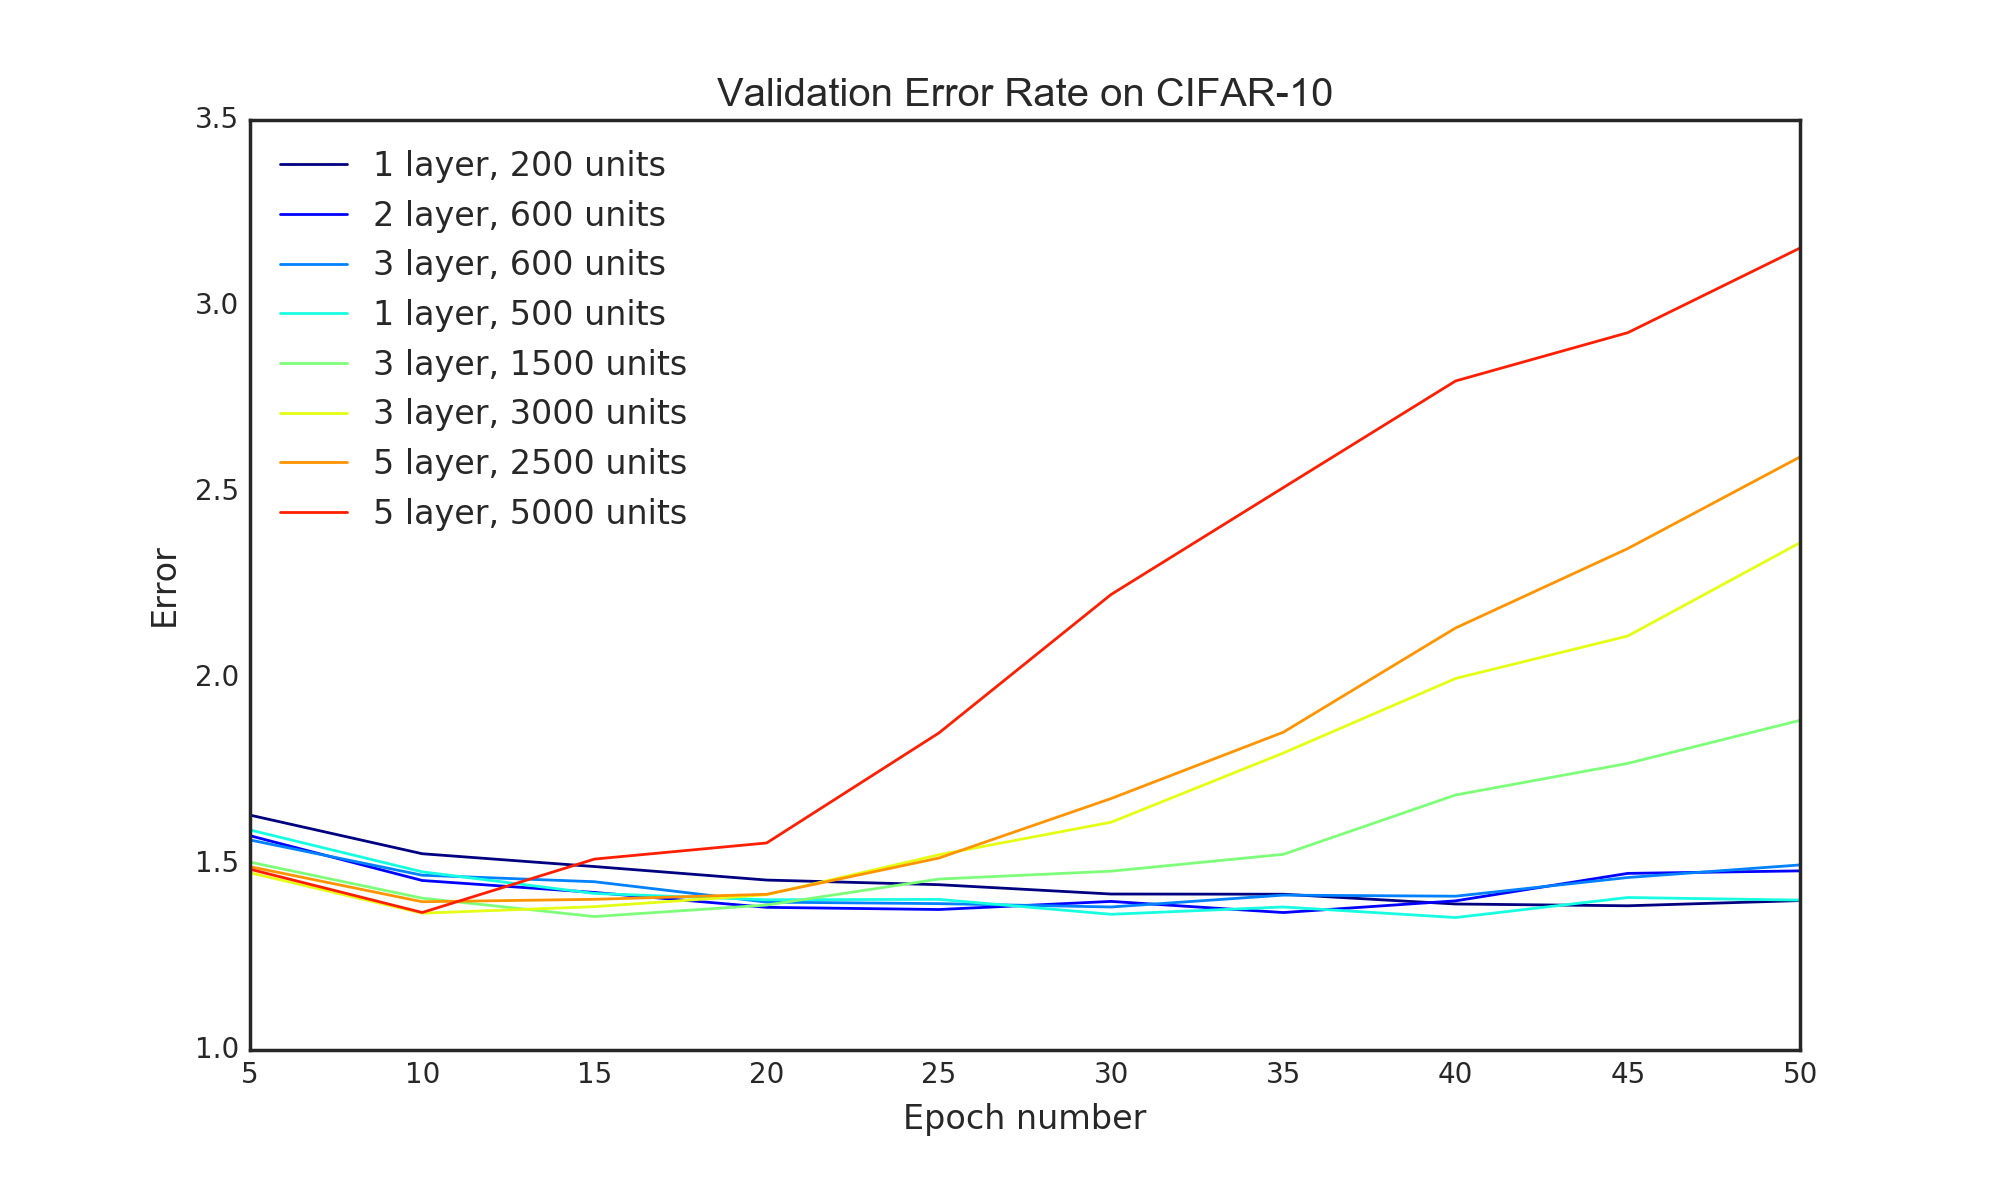
\includegraphics[width=3in]{NN_architures_valid_err}

From the plots and results of the experiments on CIFAR-10, we could find that the deeper and wider networks could get better results although they are over-fitting quickly. This is consistent with what is mentioned earlier. Since more complex network structure could provide more complex model, a deeper or wider network can do well in recognition task. Of course, to train more complex network in further work, we need to use some techniques to prevent over-fitting. 

Because the plots on CIFAR-100 are similar to the plots on CIFAR-10, we just show the plots of CIFAR-10 for analysis. For more plots of CIFAR-100, please refer to Appendix section in the end of the report.

\begin{table}[ht]
\centering 
\caption{Average Time Cost for Training Networks}
\begin{tabular}{c c c c c c}
\toprule
No. & Architecture & Average training time for each epoch(s) \\
\midrule
1 & 1 layer, 200 units &  7.96  \\
2 & 1 layer, 500 units &  16.36 \\
3 & 2 layer, 600 units &  11.79 \\
4 & 3 layer, 600 units &  8.90  \\
5 & 3 layer, 1500 units & 20.54 \\
6 & 3 layer, 3000 units & 46.66 \\
7 & 5 layer, 2500 units & 25.57 \\
8 & 5 layer, 5000 units & 63.99 \\
\bottomrule
\end{tabular}
\end{table}

From table 2, one interesting thing here is that training networks with same number of hidden units, shallow architecture will cost less time than deep architecture (see experiments no.3 and no.4). Why is that? I think one of the reasons for this phenomenon is the number of parameters in the neural network. In the 2 layers network, there are $3072 \times 300 + 300 \times 300 + 300 \times 10 = 1,014,600$ weights parameters. And in the 3 layers network, there are $3072 \times 200 + 200 \times 200 + 200 \times 200 + 200 \times 10 = 696,400$ weights parameters. Hence, to update all the weight parameters in each epoch, the shallow network will cost more time. Moreover, we could find that the networks with same number of hidden units could achieve similar recognition results. Therefore, building a deeper neural network could effectively achieve good results.

However, by comparing the experiments 2, 5 and 7, we could find that if we add two hidden layers to a one layer network, we will get a improved accuracy of 53.89\%. And if we continue to add another two hidden layers, the accuracy gets lower(51.08\%). The follow-up question here is that is there any disadvantages if we just extend the depth of neural network. He(2015) says that a notorious problem in training deep neural network is the vanishing/exploding gradients(also see Glorot(2010) and Michael Nielsen's online book), which seems similar to our phenomenon. The reason to this problem is because that the gradient tends to get smaller as we move backward through the hidden layers, which means that neurons in the earlier layers learn much more slowly than neurons in later layers. So, the neurons in the earlier layers are not well-trained enough through the whole training process.

For further work, to solve vanishing gradient problem, we could try initializing the parameters before training. Such normalisation methods can effectively solve these problems. In further experiments, we can use different normalisation methods(eg. randomly initialized the weight and biases in the network) to see if they could make a deeper neural network perform better.

\section{Activation Function}
\subsection{Research Question}
One widely used neuron activation function is sigmoid function, which is defined as:
\begin{equation*}
\sigma(z) = \frac{1}{1+exp(-z)}
\end{equation*}
 
%%sigmoid
According the equation, we could see that when the neuron's output is close to 1, the curve gets very flat, and so $\sigma'(z)$ gets very small(Michael Nielsen, Chapter 3, 2015). Then, in the training process, $\partial C/\partial w$ and $\partial C/ \partial b$ get very small that the updating on weights and bias gets very small. This is the origin of the learning slowdown. Also, because of the characteristics of sigmoid function, all weights to the same neuron must either increase together or decrease together. That's a problem, since some of the weights may need to increase while others need to decrease. That can only happen if some of the input activations have different signs. So, using different kinds of activation function would make the networks learn faster, generalize better to test data, or perhaps do both depending on the application.

In the experiments, we will try two alternative activation function: Tanh and ReLU. 

For tanh activation function:
\begin{equation*}
    \tanh\left(z\right) = 
    \frac{\exp\left(z\right) - \exp\left(-z\right)}{\exp\left(z\right) + \exp\left(-z\right)}
\end{equation*}

For ReLU activation function:
\begin{equation*}
    ReLU(z) = 
    \max\left(0,\,z\right)
\end{equation*}

Both tanh and ReLU could obtain negative values so they don't have problem of monotonically updating weights and bias. However, the exponential operation in tanh would consume a lot of computing resources. Instead, ReLU would be better since it only has a maximum operation. So, in this section, we will do some experiments to evaluate the performance of sigmoid, tanh and ReLU. So, for further work, it is worth trying to continue using ReLU function. In the rest of the baseline experiments, we will also use ReLU function.

\textbf{Research question 1:} How's the performance of these activation functions?

\textbf{Research question 2:} What are the properties that lead to a good activation function?

\subsection{Method}
For better understanding the activation, we plot the images of each function first:

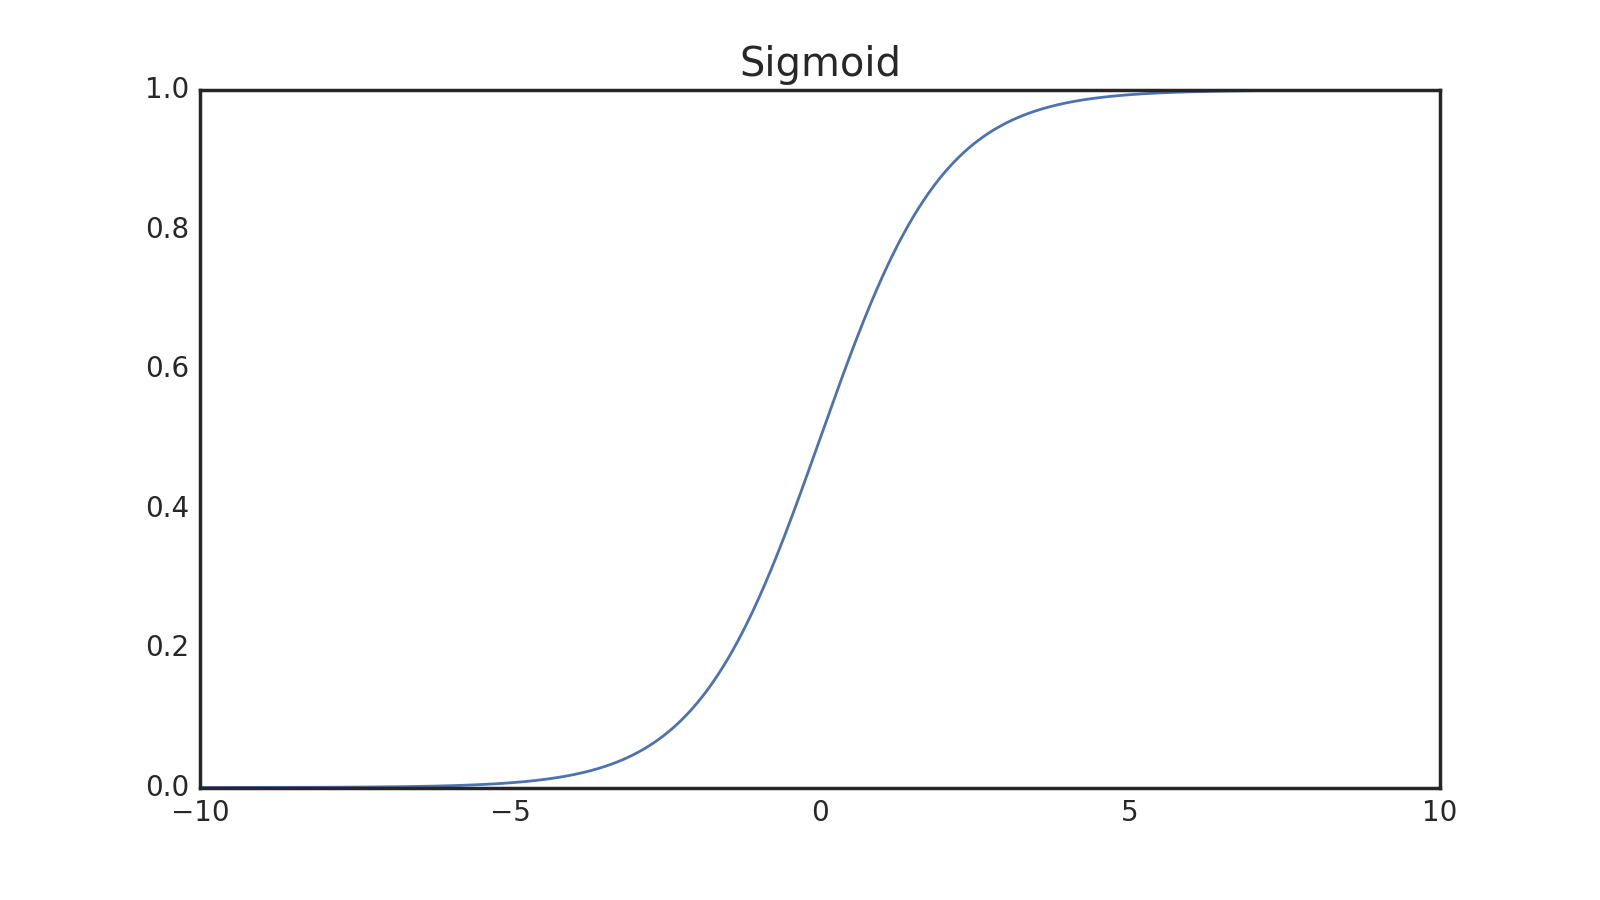
\includegraphics[width=2in]{Sigmoid}
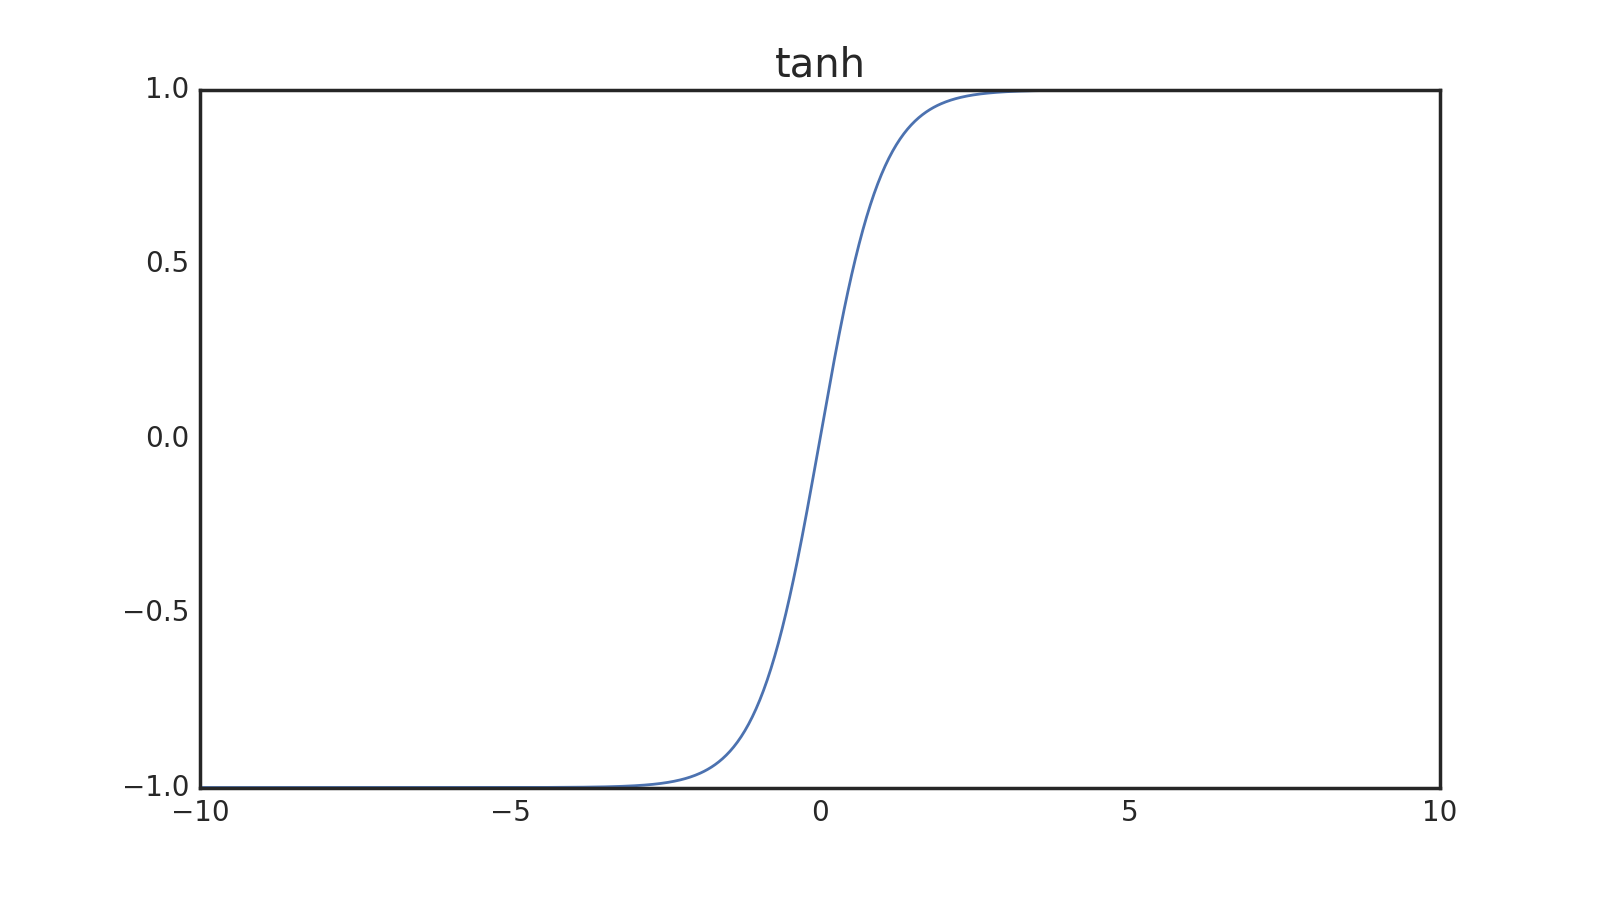
\includegraphics[width=2in]{tanh}
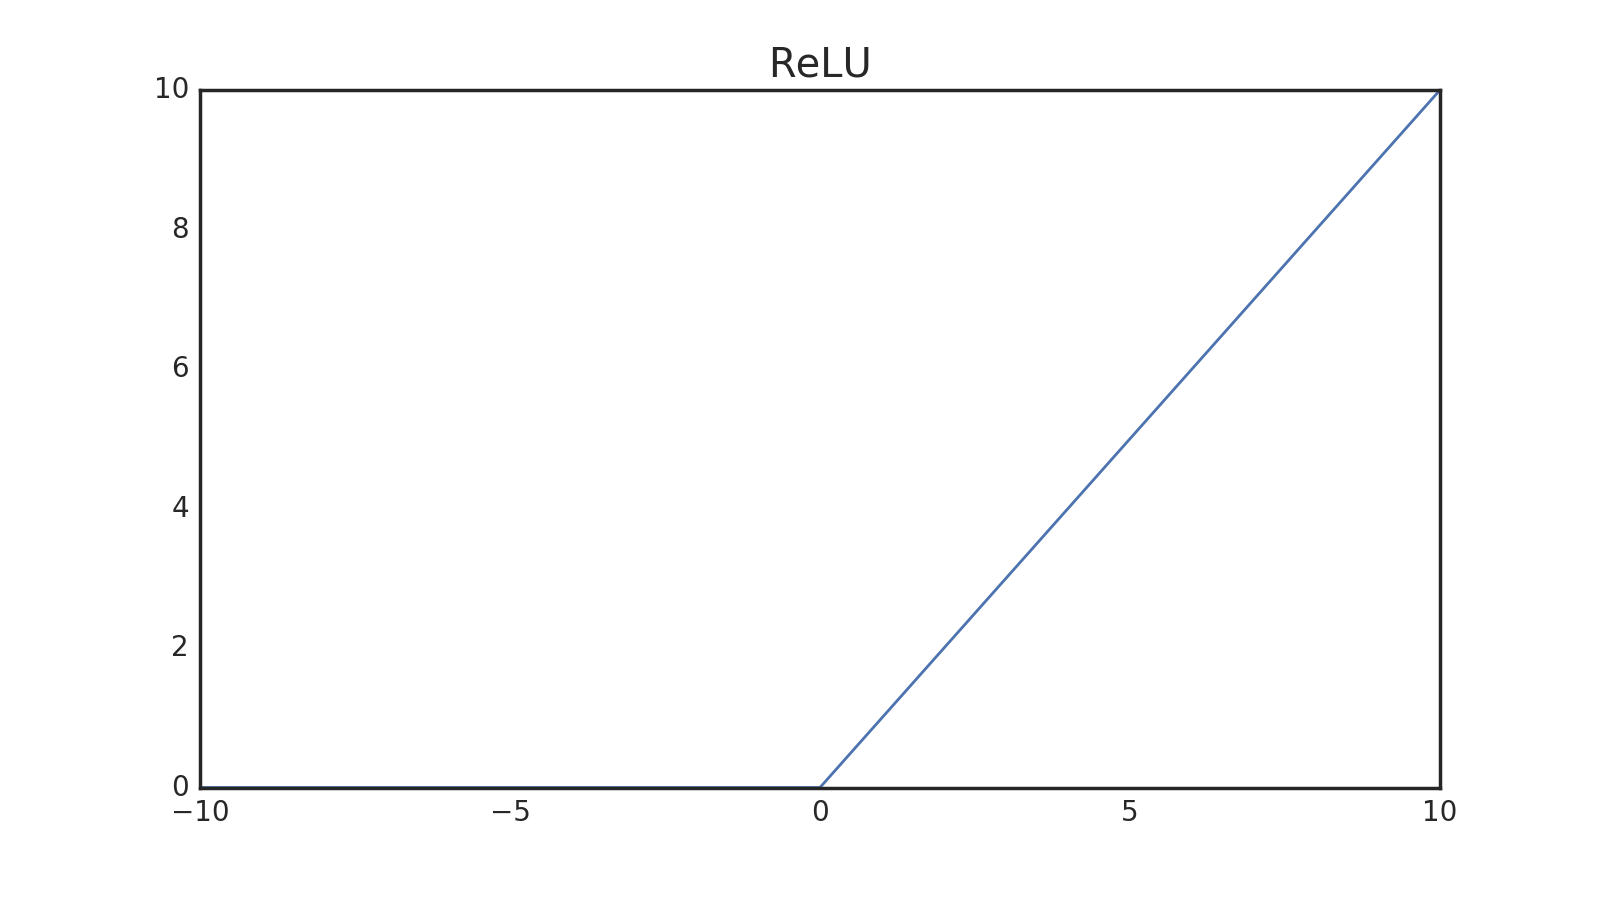
\includegraphics[width=2in]{ReLU}

As for the implementation part, we could just modify the definition of fully connected layer to change the activation function of neural networks. For example, if I set sigmoid as our activation function, the definition of layer function should be:

\emph{def fully\_connected\_layer(inputs, input\_dim, output\_dim, nonlinearity=tf.nn.relu)}

To compare different activation function, we will apply sigmoid, tanh and ReLU to a standard network(3 hidden layers, 200 units each layers). For the training process, we use $AdamOptimizer$(learning rate = 0.0001, $\epsilon = 0.001$) as training method and sigmoid cross entropy as error function. The experiments design and some basic results are shown as below:
\begin{table}[!ht]
\centering 
\caption{Experiment Design for Different Activation Function}
\begin{tabular}{c c c c c c}
\toprule
Dataset & Method & Unit type & Architecture & Error & Average training time(s)  \\
\midrule
\multirow{3}{*}{CIFAR-10} & NN & sigmoid & 3 layer, 600 units & 1.45 & 11.53   \\
& NN & tanh & 3 layer, 600 units & 1.46 & 11.50   \\
& NN & ReLU & 3 layer, 600 units & 1.49 & 11.53   \\
\midrule
\multirow{3}{*}{CIFAR-100} & NN & ReLU & 3 layer, 600 units & 3.29 & 12.11 \\
& NN & tanh & 3 layer, 600 units & 3.29 & 11.87   \\
\bottomrule
\end{tabular}
\end{table}

\subsection{Results and Discussion}
By plotting the training and validation data, the evolution of training process can be observed. The results on CIFAR-10 are shown in below plots.

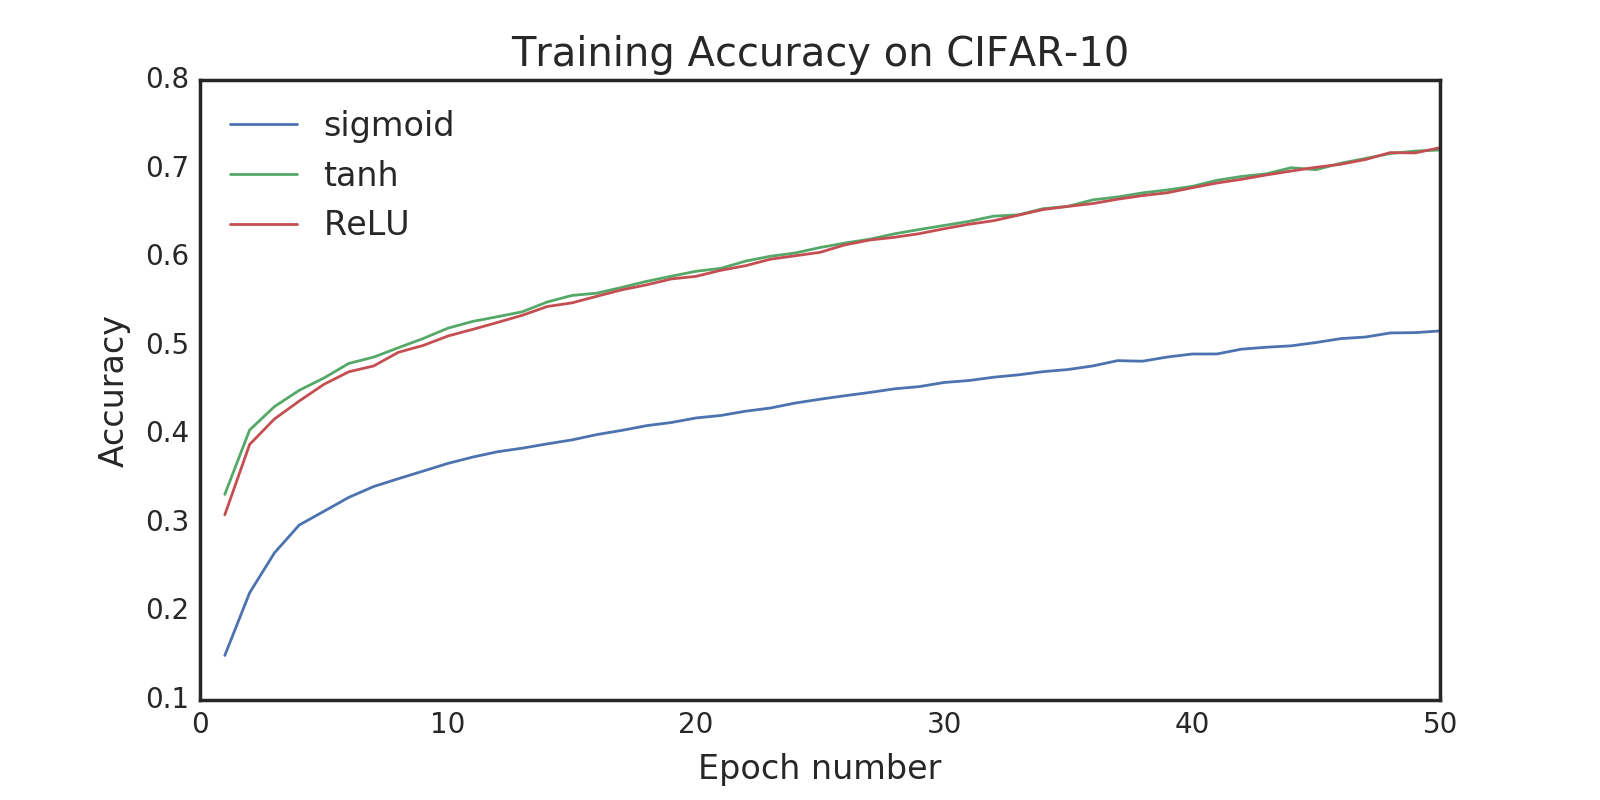
\includegraphics[width=3in]{activation_function_train_acc}
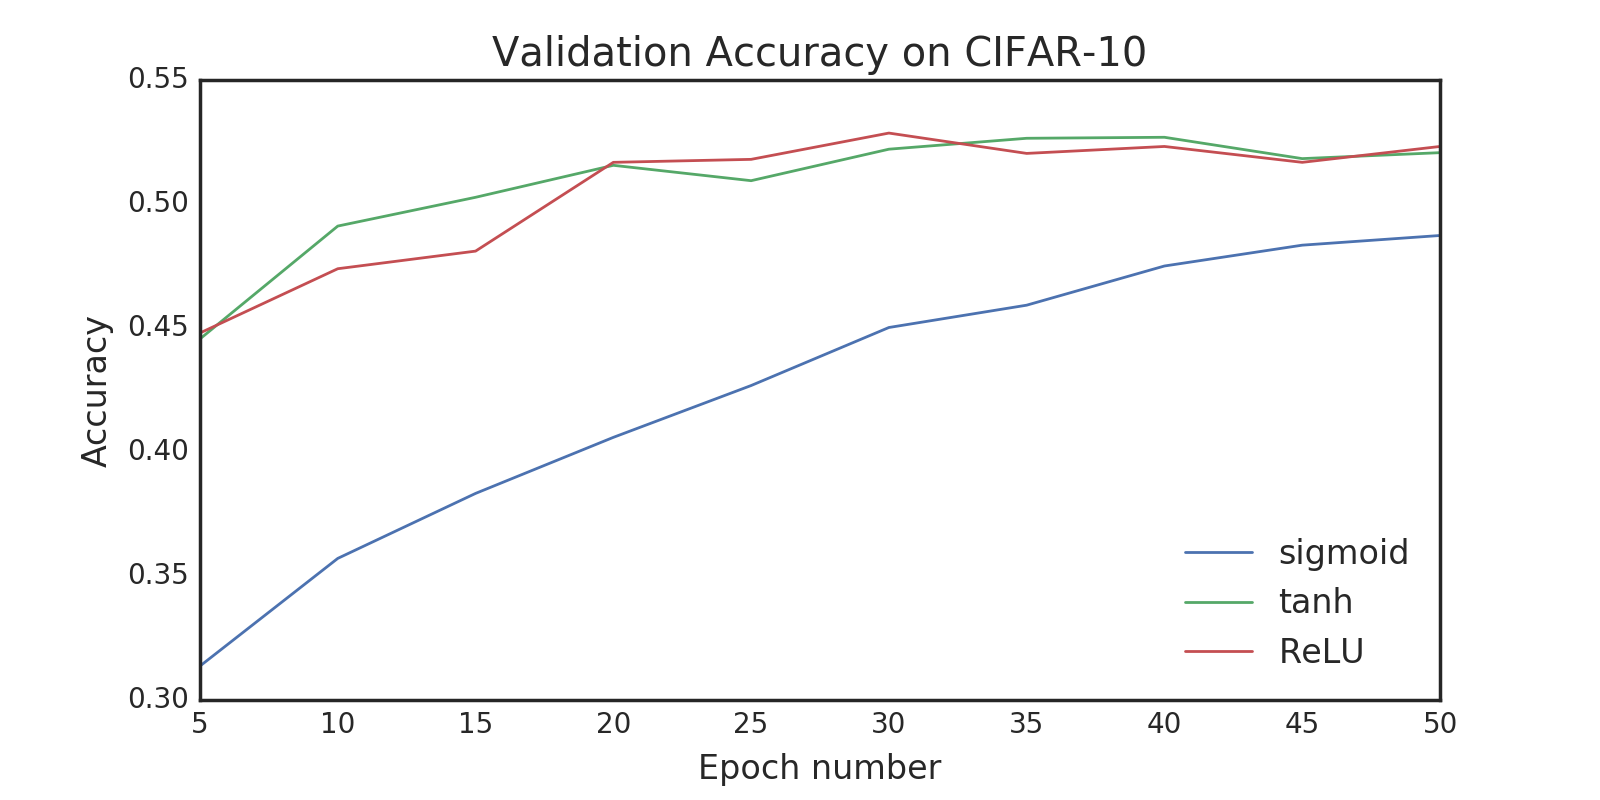
\includegraphics[width=3in]{activation_function_valid_acc}

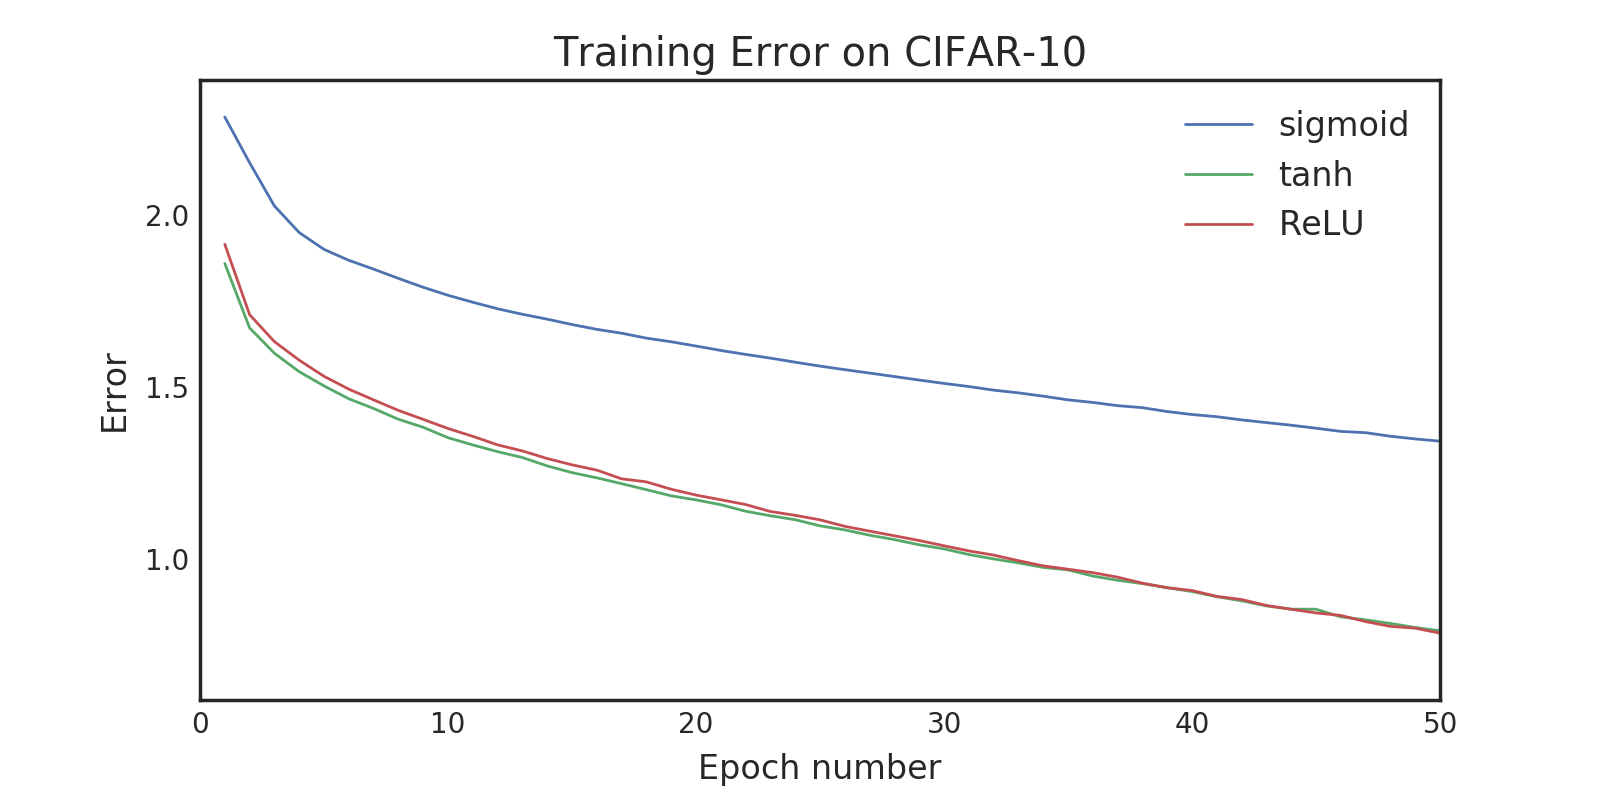
\includegraphics[width=3in]{activation_function_train_err}
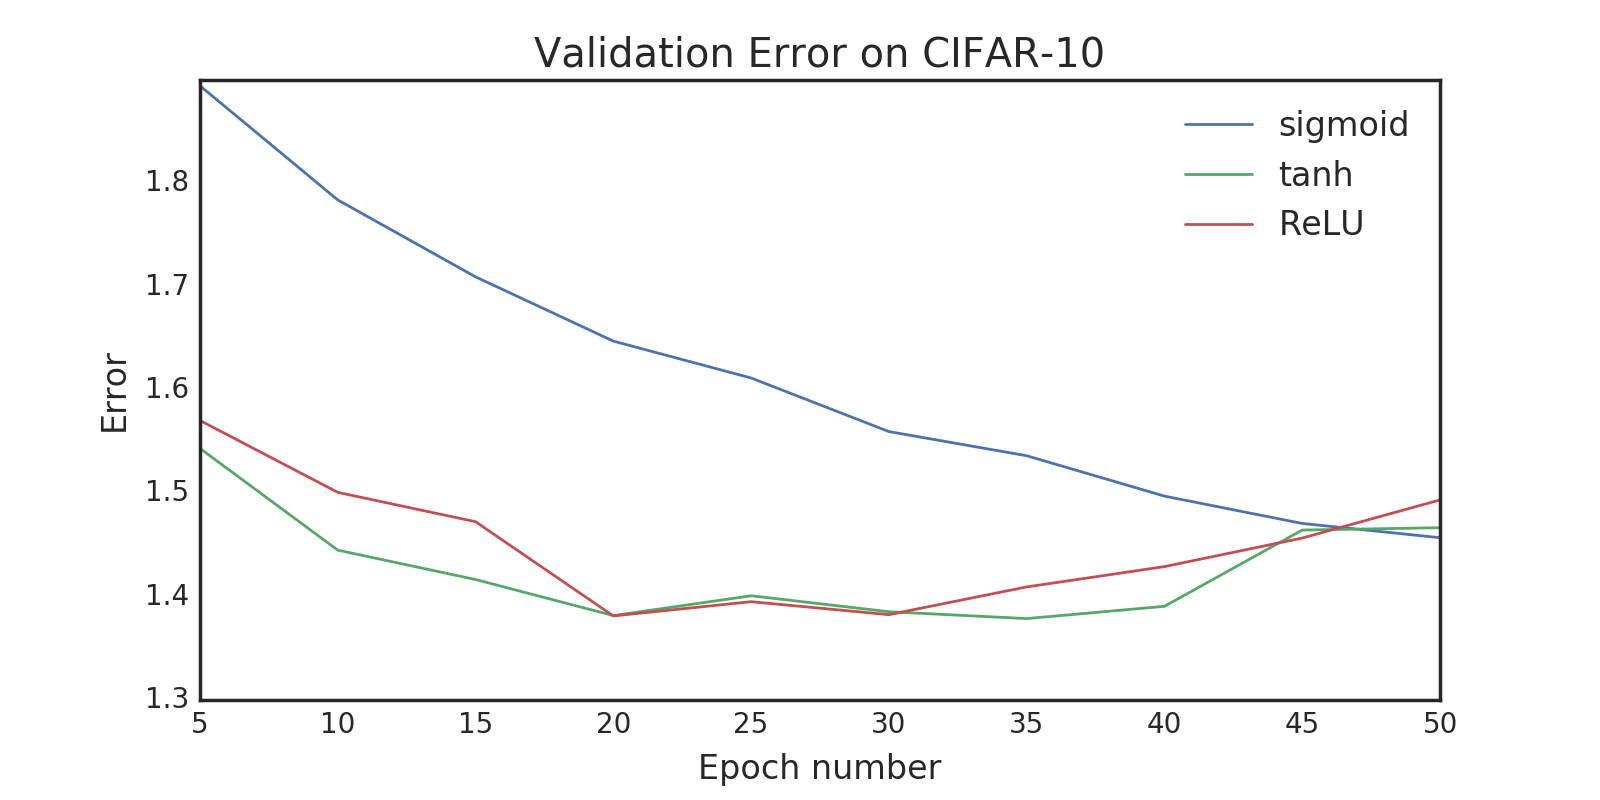
\includegraphics[width=3in]{activation_function_valid_err}

The plots show that the results are consistent with our previous ideas. It is obvious that sigmoid function performs worse than other activation functions. Also, tanh and ReLU leans faster and generates better result than sigmoid. This is because the sigmoid function updates the weights parameters monotonically, and this slow down the training process.
Below are the results on CIFAR-100:

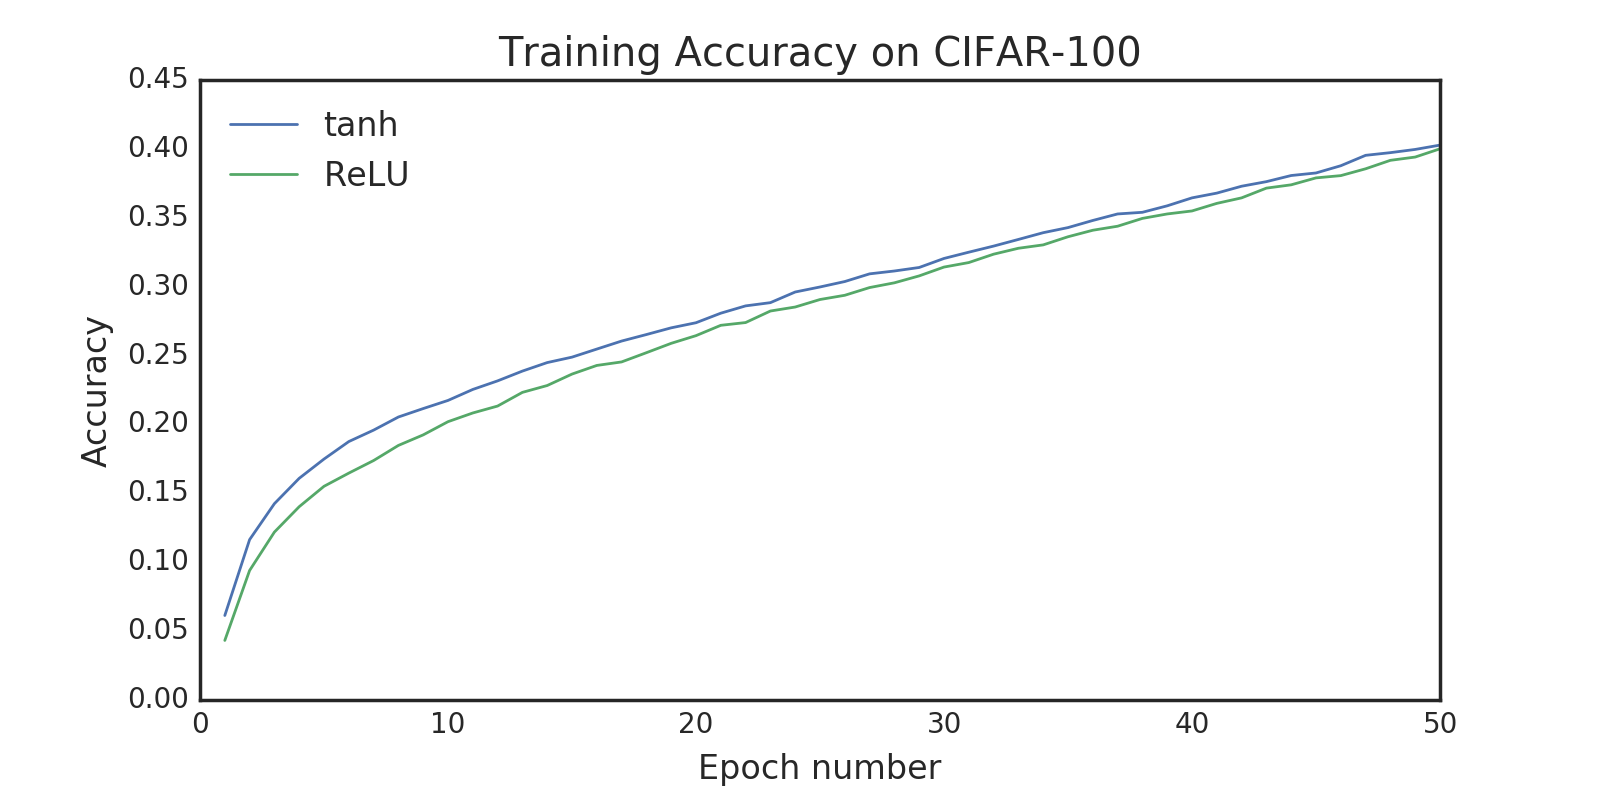
\includegraphics[width=3in]{activation_function_train100_acc}
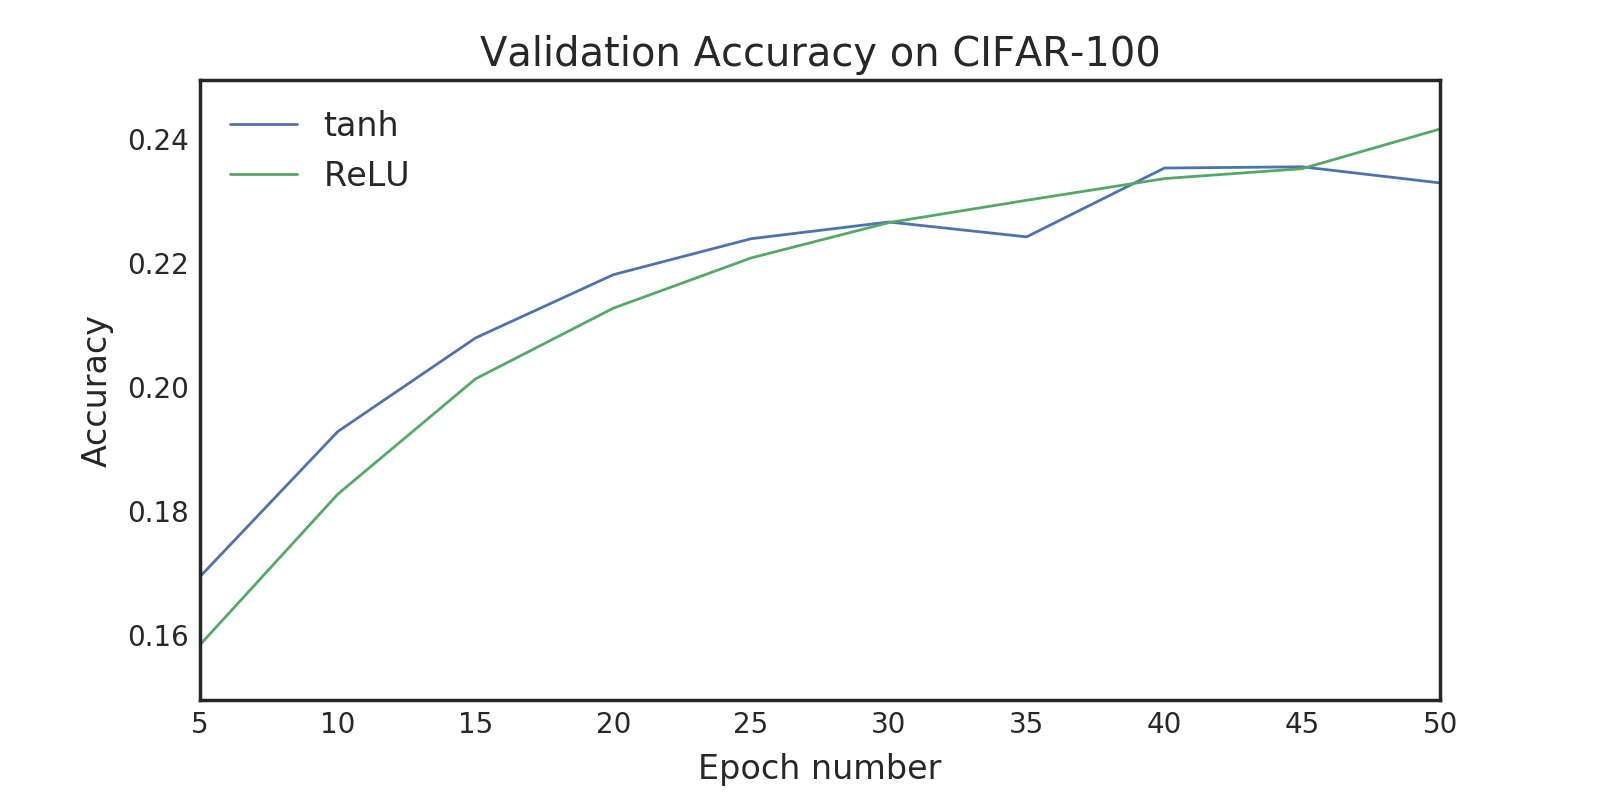
\includegraphics[width=3in]{activation_function_valid100_acc}

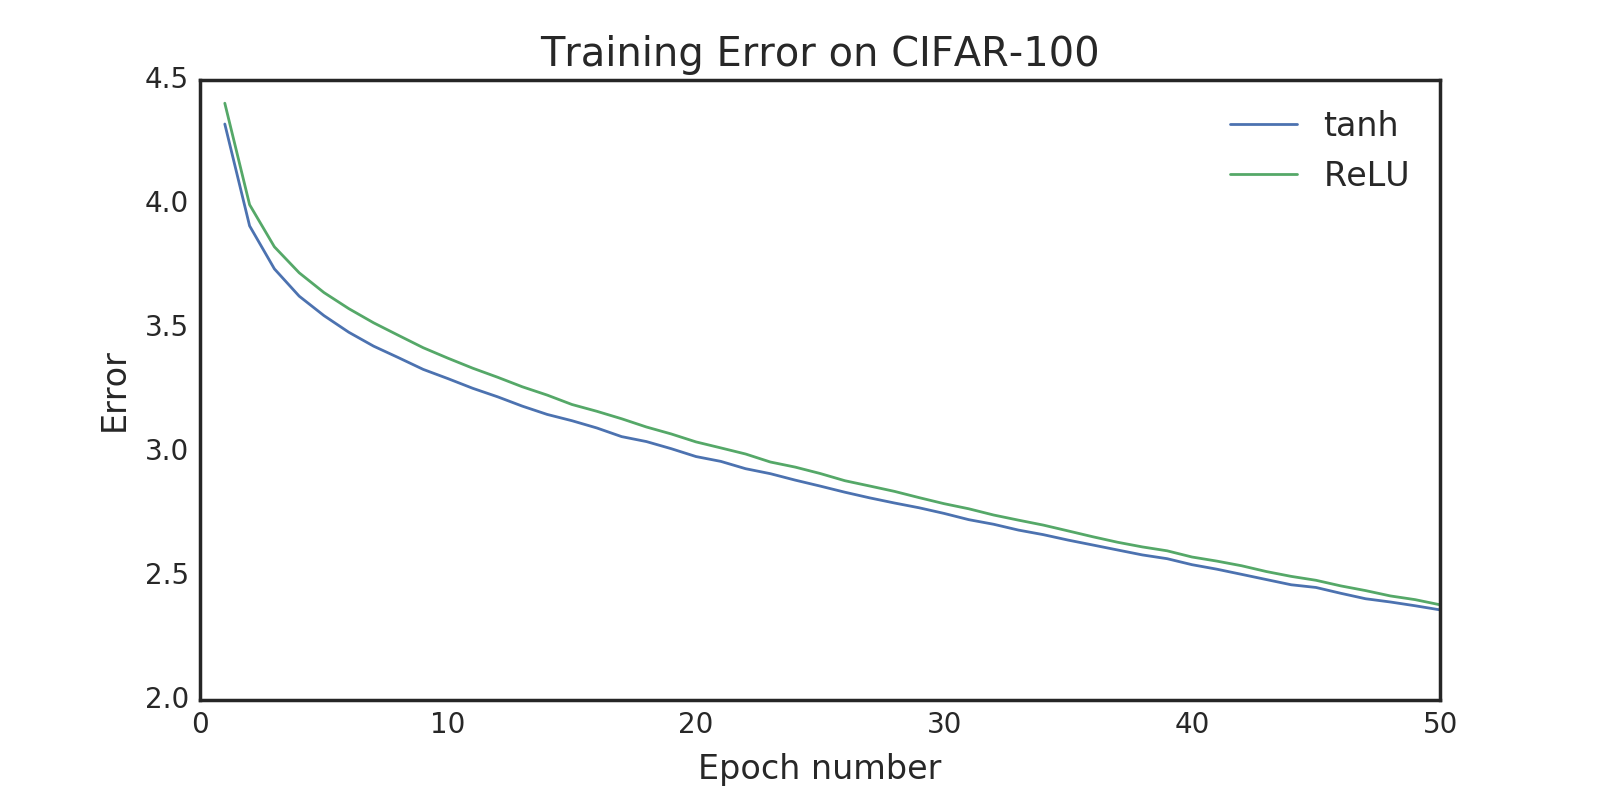
\includegraphics[width=3in]{activation_function_train100_err}
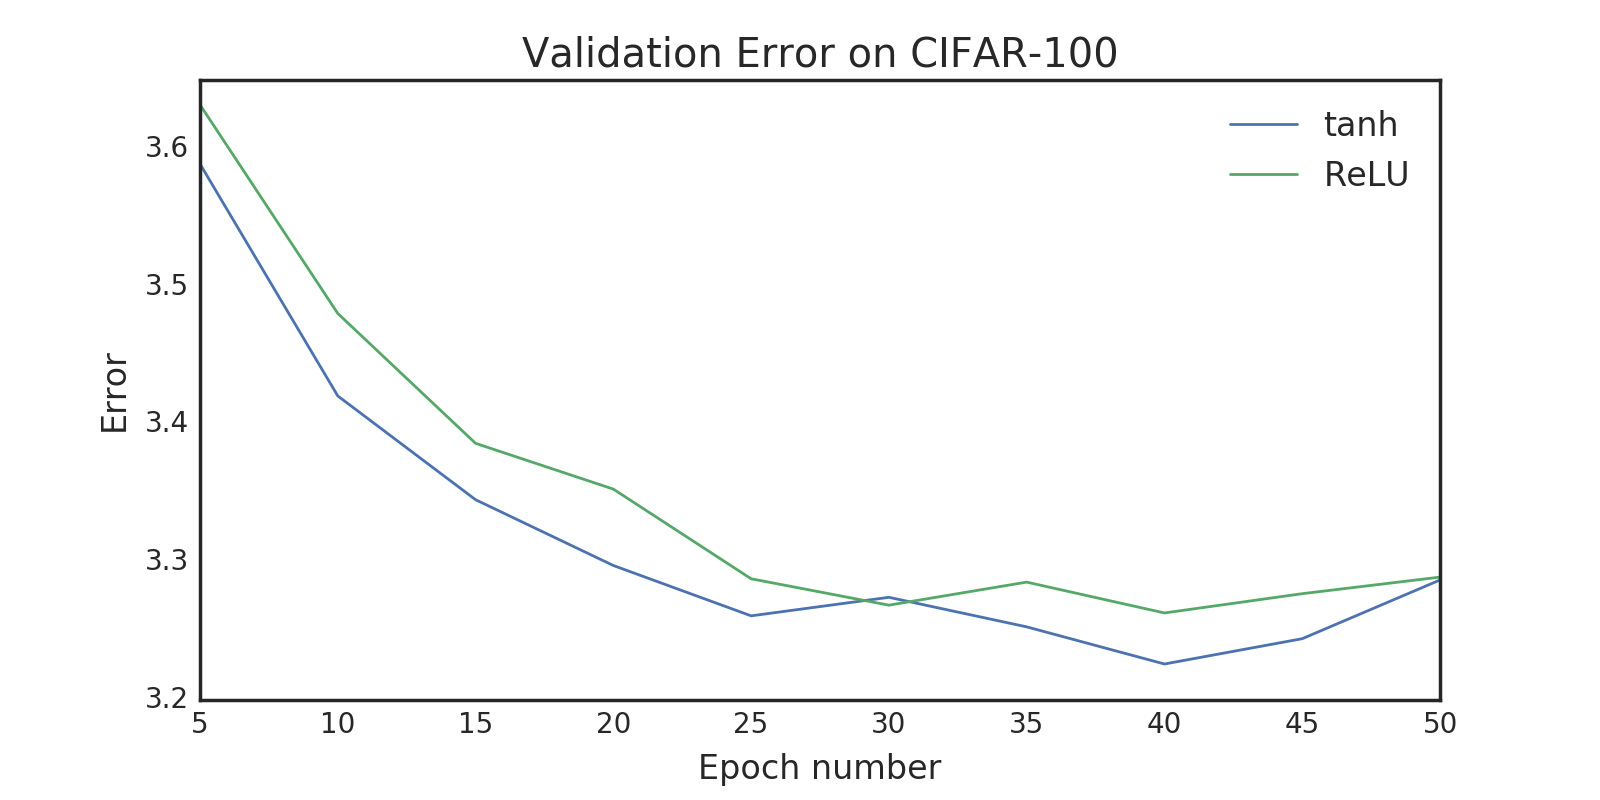
\includegraphics[width=3in]{activation_function_valid100_err}

The experiments on CIFAR-100 also give the similar results. By comparing the final accuracy, ReLU seems to be the best activation function. So, what properties make ReLU work so well? Xu(2015) says in his paper, the superior performance of ReLU comes from the sparsity, which means that the activations are sparse after pass ReLU. Let's move back to ReLU itself. The ReLU function is a piecewise linear function which prunes the negative part to zero and retains the positive part. The function makes the network sparse enough so that the performance gets better. 

Lecun(2015) also says in his paper, the ReLU typically learns much faster 
in networks with many layers, allowing training of a deep supervised 
network without unsupervised pre-training. However, we couldn't obtain this result through our experiments because our experimental architectures are not deep enough that the good properties of ReLU can not be reflected. For further experiments, we could try deep neural network with ReLU to see if it could learn faster in networks.

\section{Normalisation}
\subsection{Research Question}
Batch normalisation is the process of using minibatch statistics to normalise activations of each layer. The batch normalisation layer is defined like:
\begin{align*}
& \widehat{u_i} = \frac{u_i - \mu_i}{\sqrt{\sigma_i^2 + \varepsilon}} 
  \quad , \quad z_i = \gamma_i \widehat{u_i} + \beta_i = batchNorm(u_i)
\end{align*}

Where the $\mu_i$ and $\sigma_i^2$ are the mean and variance over the complete training data.
\begin{align*}
& \mu_i = \frac{1}{M} \sum_{m=1}^{M} u_i^m \quad , \quad
  \sigma_i^2 = \frac{1}{M} \sum_{m=1}^{M}(u_i^m-\mu_i)^2 
\end{align*}

Batch normalisation has a lot of advantages. It can be applied to convolutional networks and accelerate the training process, which is a valuable point in future work. According to He(2015), convolutional networks could get very good results on CIFAR-10 and CIFAR-100 dataset. Hence, I'm planning to try convolutional networks in next coursework. Continuing using batch normalisation is a good way to train many-layered networks easier. So, in this part, we will apply batch normalisation to our baseline network to see whether it could speed up the training process.

\textbf{Research question:} Does batch normalisation speed up the training process?

\subsection{Method}
\textbf{Implementation for batch normalisation:} To use tensorflow function $tf.nn.batch\_normalizatioin$, we need to calculate the mean and variance of the data by using $tf.nn.moments$. The definition of the BN layer is:

\emph{def \ BN\_layer(inputs, input\_dim, phase\_train, scope='bn')}

Where the $inputs$ is the outputs of previous hidden layer, $input\_dim$ is the dimension of $inputs$, $phase\_train$ is a global variable to adjust whether or not to use batch normalisation. For detailed implementation of batch normalisation, please refer to notebook 09a\_Object\_recognition\_with\_CIFAR-10\_BN.

To evaluate the performance of batch normalisation, we applied it to two different neural networks and did some comparable experiments. For the training process, we use $GradientDescentOptimizer$ and set learning rate to $0.0001$.By setting a very low learning rate, we could easily investigate the performance of batch normalisation networks. The design of experiments and some basic results are shown below:

\begin{table}[!ht]
\centering 
\caption{Experiment Design for Batch Normalisation}
\begin{tabular}{c l c c c c }
\toprule
No. & Method & Unit type & Architecture & Err.(CIFAR-10) & Err.(CIFAR-100)  \\
\midrule
1 & NN & ReLU & 3 layer, 600 units & 1.79 & 4.32 \\
2 & NN & ReLU & 5 layer, 1000 units & 1.78 & 4.39   \\
3 & NN + BN & ReLU & 3 layer, 600 units & 1.76 & 4.13   \\
4 & NN + BN & ReLU & 5 layer, 1000 units & 1.82 & 4.18   \\
\bottomrule
\end{tabular}
\end{table}

\subsection{Results and discussion}
The evolution plots are shown below:

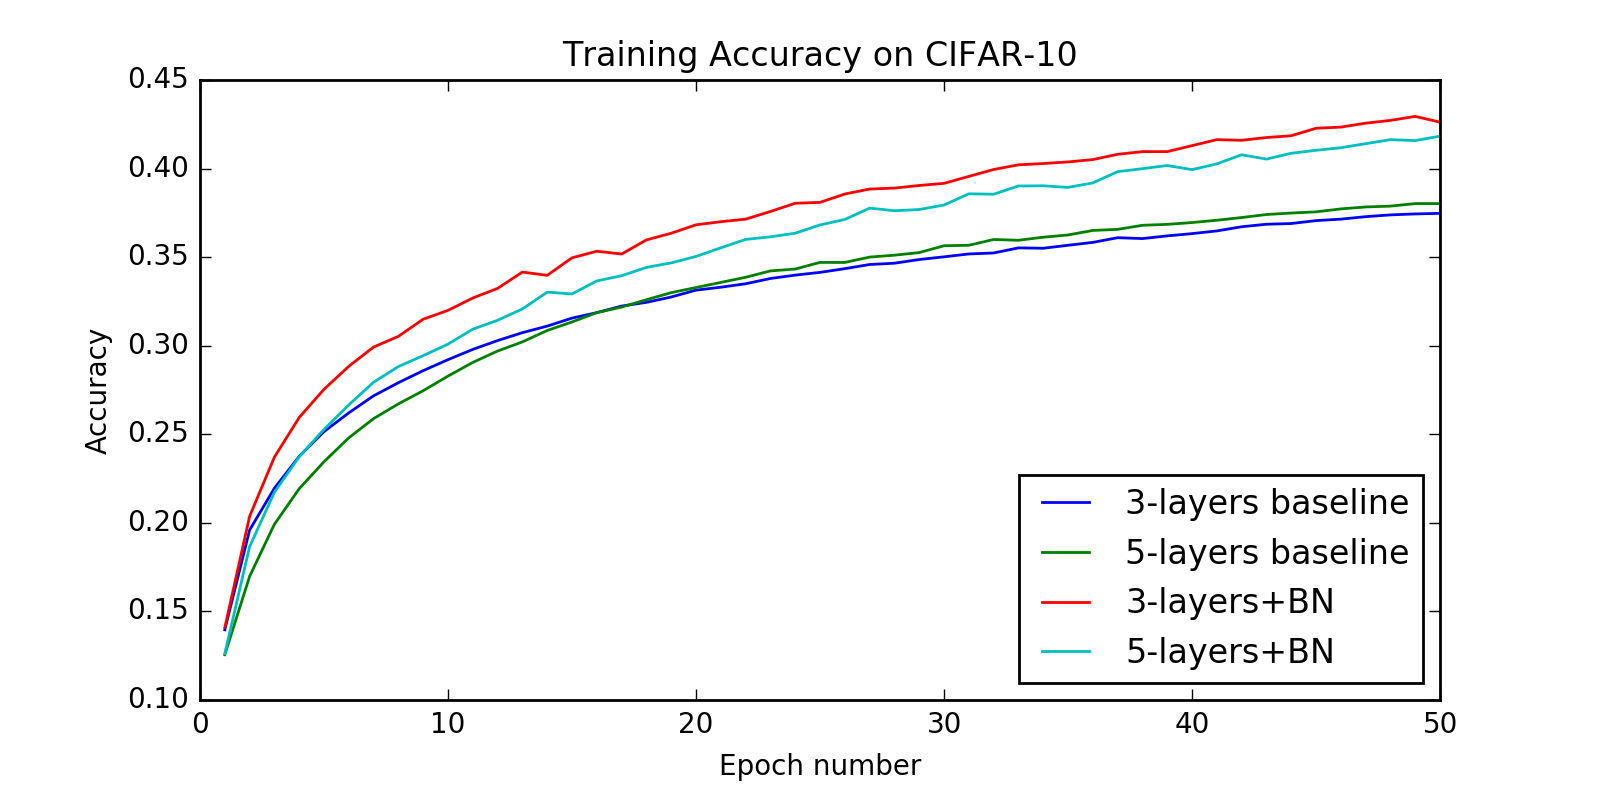
\includegraphics[width=3in]{BN_train_acc}
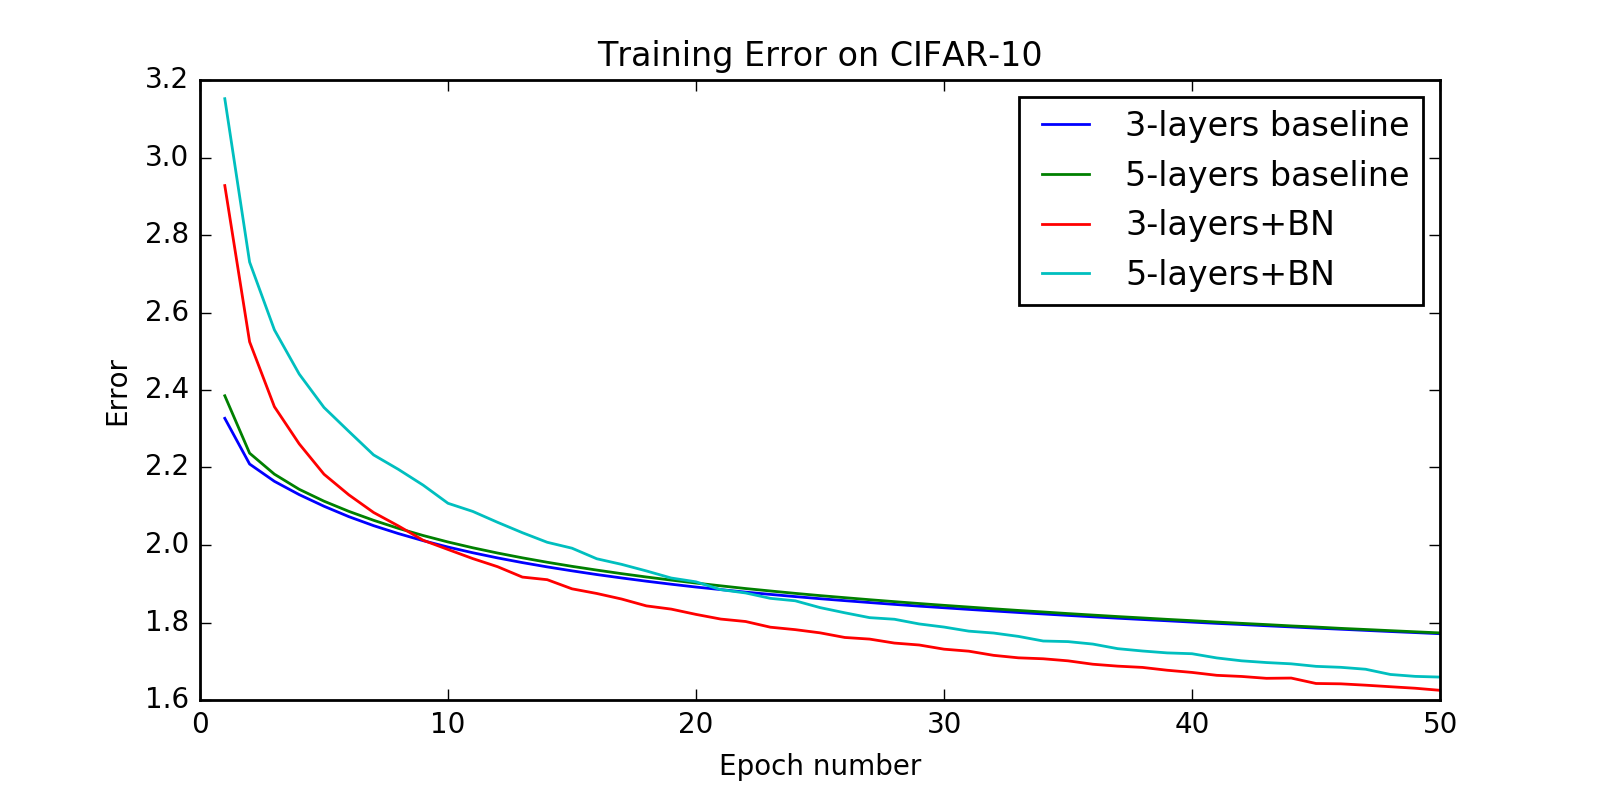
\includegraphics[width=3in]{BN_train_err}

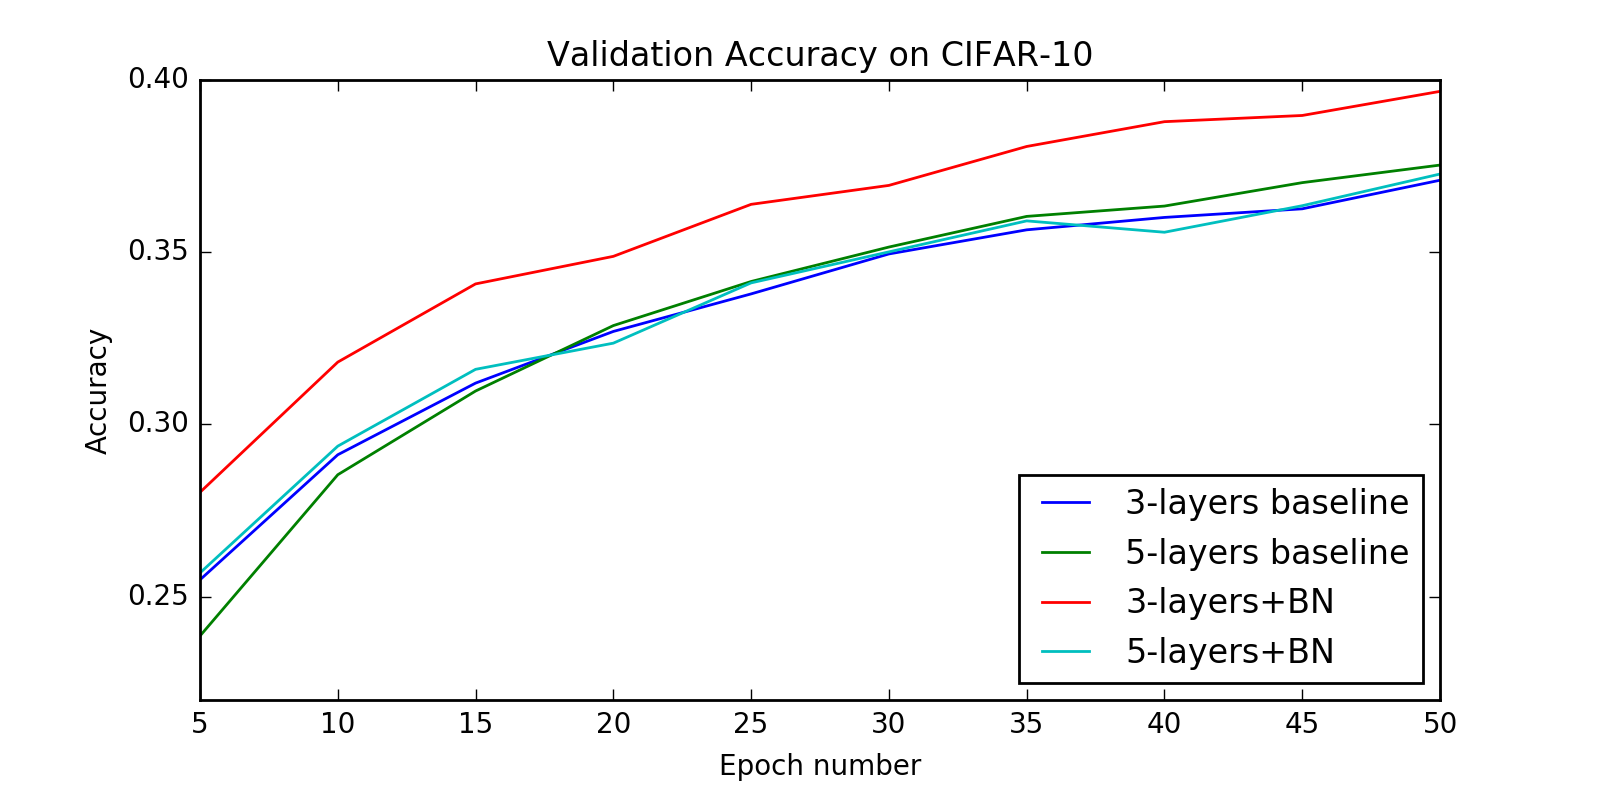
\includegraphics[width=3in]{BN_valid_acc}
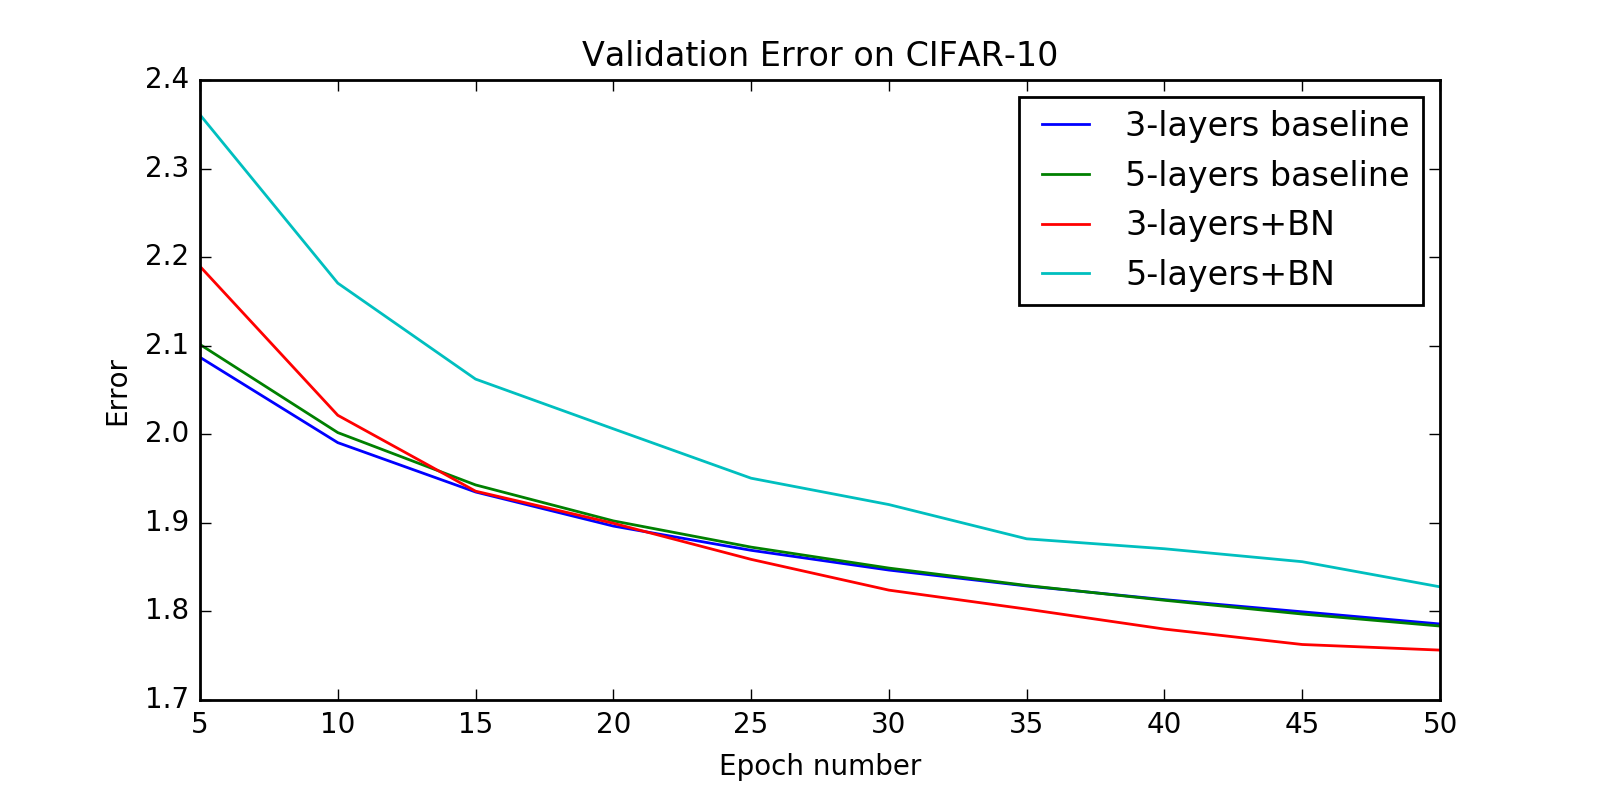
\includegraphics[width=3in]{BN_valid_err}

As what is shown in the training plots, BN dramatically accelerate the training of neural networks and also achieve a good recognition accuracy. This is important in future work for the reason that we will definitely extend deeper networks in further experiments. When the neural network structure becomes more complex, training network will become complicated and time consuming because the learning speed of each layer changes while updating the weights parameters. This extremely slows down the training process by applying a small learning rate to make each layer well-trained. Ioffe indicates that BN could provide very good performance in training deep neural network and it could also play the role of regularisation. The networks could benefit a lot from both of these good properties.

However, as is shown in the data, BN networks don't provide good accuracy. Hence, it is necessary to combine BN with other techniques for reaching better results in future experiments.

For experiments results of CIFAR-100 (which are more convincing on improving the performance of NN) , please see appendix in the end of the report.

\section{Regularisation}
\subsection{Research Question}
L1 and L2 Regularisation is used to decay weights by adding a complexity term $E_w$ to the network error function so that we could allow the data to determine how to reduce the effective number of parameters. It is defined as:
\begin{eqnarray*}
   E^\star =  \underbrace{\bar{E}}_{\textrm{data term}} + \underbrace{C}_{\textrm{complexity term}} \\
   For \ L1 \ regularisation: C = \beta \sum_{i} \left | w_i \right | \\
   For \ L2 \ regularisation: C = \beta \frac{1}{2}\sum_{i} w_i^2 
\end{eqnarray*}

Both L1 and L2 regularisation could control the effective flexibility to avoid either overtraining or undertraining. In the experiments, we will apply both of them to the baseline networks to see if they could help to improve the performance. 

As for dropout, it is a way of training networks to behave so that they have the behaviour of an average of multiple networks. In each mini-batch, dropout training will randomly delete a fraction of hidden units and their related weights and biases so that the training process could cover different part of the network in each batch. This approach could effectively avoid overtraining and undertraining. In the experiments, we will also try dropout training and combine it with L1 and L2 regularisation to investigate how it could help to improve the performance.

\textbf{Research question 1:} How these regularisation methods influence the training process?

\textbf{Research question 2:} Focusing on dropout, does dropout work improve the recognition results? And investigating more about dropout.

\subsection{Methods}

\textbf{Implementation for L1 regularisation:} \ According to the equation of L1 regularisation, we need to calculate the absolute values of weights and add them together. To get the weights of each layer, the definition of fully connected layer need to be modified by returning the weights each time. The code to calculate the complexity term is:

\emph{tf.reduce\_sum(tf.abs(weights))}

By adding this part to error function, we could do L1 weights decay in the training process.

\textbf{Implementation for L2 regularisation:} \ Since tensorflow has the implementation of L2 loss function ($tf.nn.l2\_loss$ function), we could just use that function to calculate the complexity term. Also, the modification on fully connected layer of L1 need to be done.

\textbf{Implementation for dropout:} \ To use dropout to train neural networks in tesorflow, we need to modify the output part of the definition of fully connected layer. The code to do this is:

\emph{$outputs = tf.nn.dropout(nonlinearity(tf.matmul(inputs, weights) + biases),keep\_prob)$}  

Also, we need a global variable $keep\_prob$ to control the training process and validation process. The modification of training and validation process could be done by changing the $feed\_dict$ part:

for training process: {$feed\_dict=\{inputs: input\_batch, targets: target\_batch, keep\_prob:0.8\}$}

for validation process: {$feed\_dict=\{inputs: input\_batch, targets: target\_batch, keep\_prob:1.0\}$}

The value of $keep\_prob$ means how many units we use in the epoch. For example, if we set $keep\_prob$ to $0.8$ in training process, it means we will randomly use $80\%$ of units for training for each epoch.

Having done the implementation of regularisation approaches, we did some related experiments on both CIFAR-10 and CIFAR-100. The design of experiments and some basic results are shown below:
\begin{table}[!ht]
\centering 
\caption{Experiment Design for L1 \& L2 Regularisation and Dropout}
\begin{tabular}{c l c c c c }
\toprule
No. & Method & Unit type & Architecture & Err.(CIFAR-10) & Err.(CIFAR-100)  \\
\midrule
1 & NN & ReLU & 3 layer, 600 units & 2.22 & 3.89 \\
2 & NN + L1 & ReLU & 3 layer, 600 units & 1.85 & 3.75   \\
3 & NN + L2 & ReLU & 3 layer, 600 units & 1.72 & 3.91   \\
4 & NN + L1L2 & ReLU & 3 layer, 600 units & 1.86 & 4.03   \\
5 & NN + Dropout & ReLU & 3 layer, 600 units & 1.35 & 3.23   \\
6 & NN + L1L2 +Dropout & ReLU & 3 layer, 600 units & 1.91 & 4.20   \\
\bottomrule
\end{tabular}
\end{table}

These experiments are designed for comparing the performance of different regularisation approaches and also the combination of these approaches. We use ReLU as standard activation function and apply regularisation approaches to a standard neural network with the structure of 3 layers, 600 hidden units. In the training process, we use $AdamOptimizer$ with the learning rate of 0.0001 and set $\epsilon = 0.001$. As for the parameters of regularisation methods, with the previous experiments on coursework 2, we directly set $\beta_1 = 0.0001$ for L1 regularisation and $\beta_2 = 0.01$ for L2 regularisation. For dropout rate, following Srivastava's work, we set dropout rate to 0.8 to see if it could get an acceptable result.

\subsection{Results and discussion}

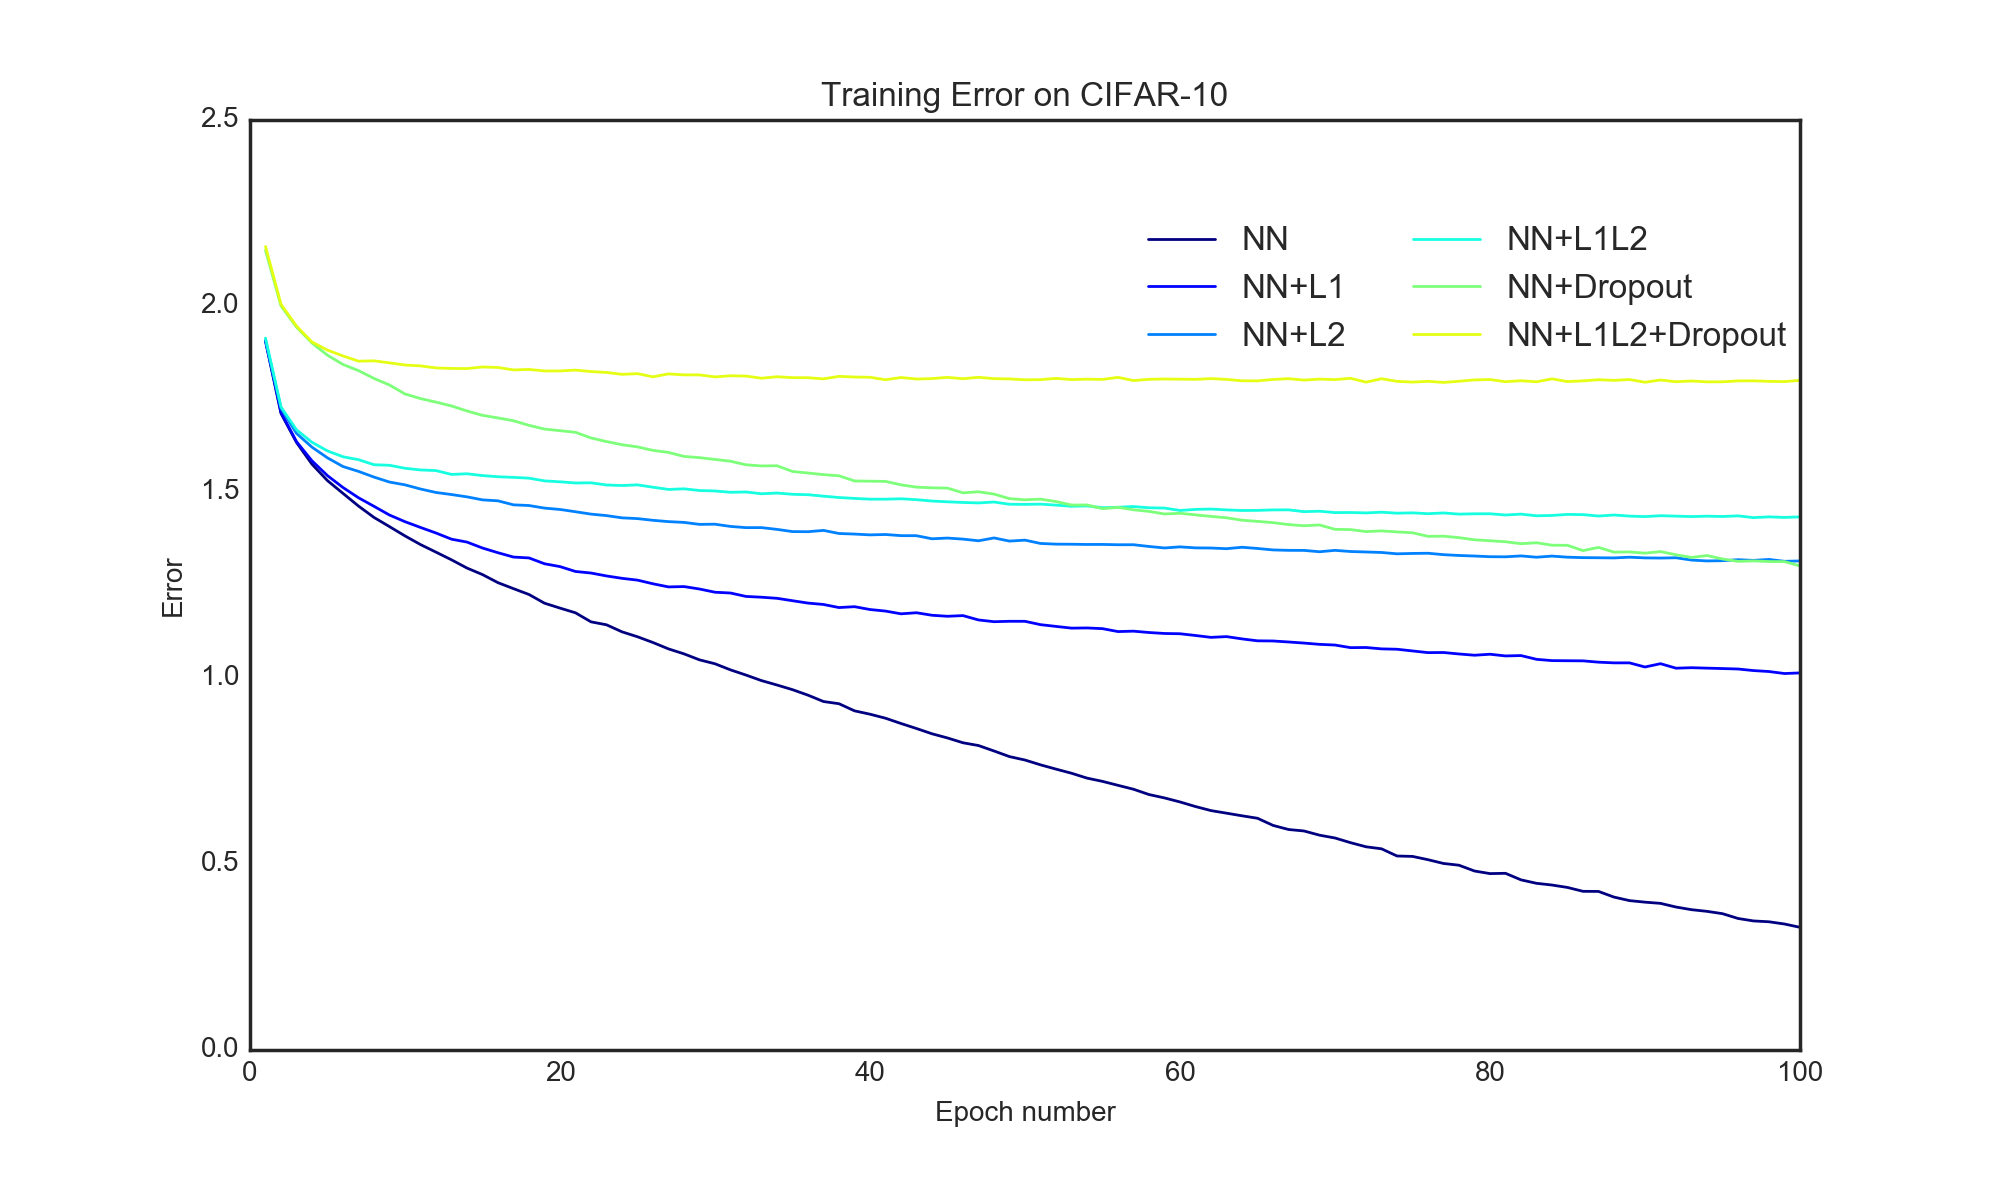
\includegraphics[width=3in]{Regularisation_train_err_2}
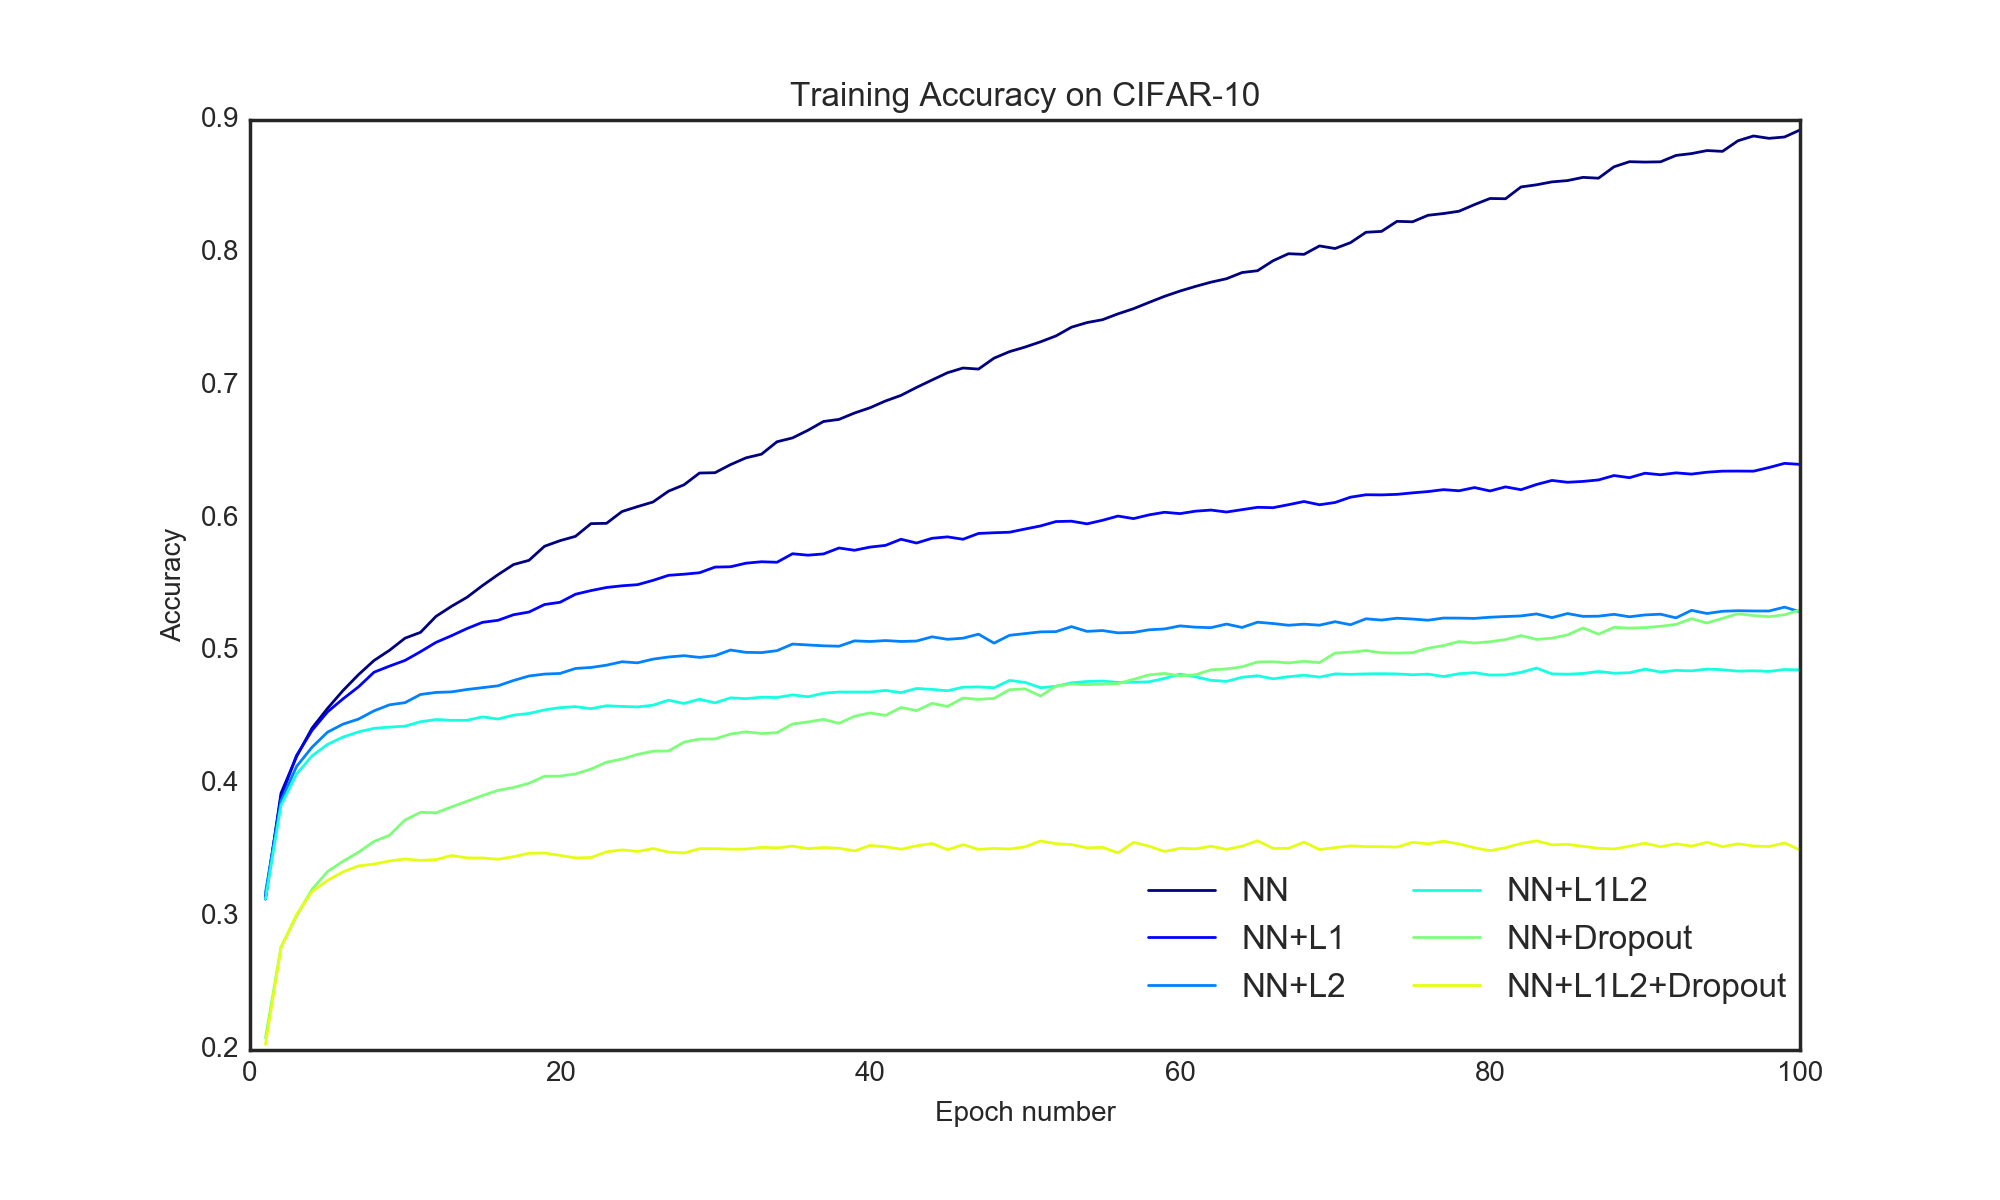
\includegraphics[width=3in]{Regularisation_train_acc_2}

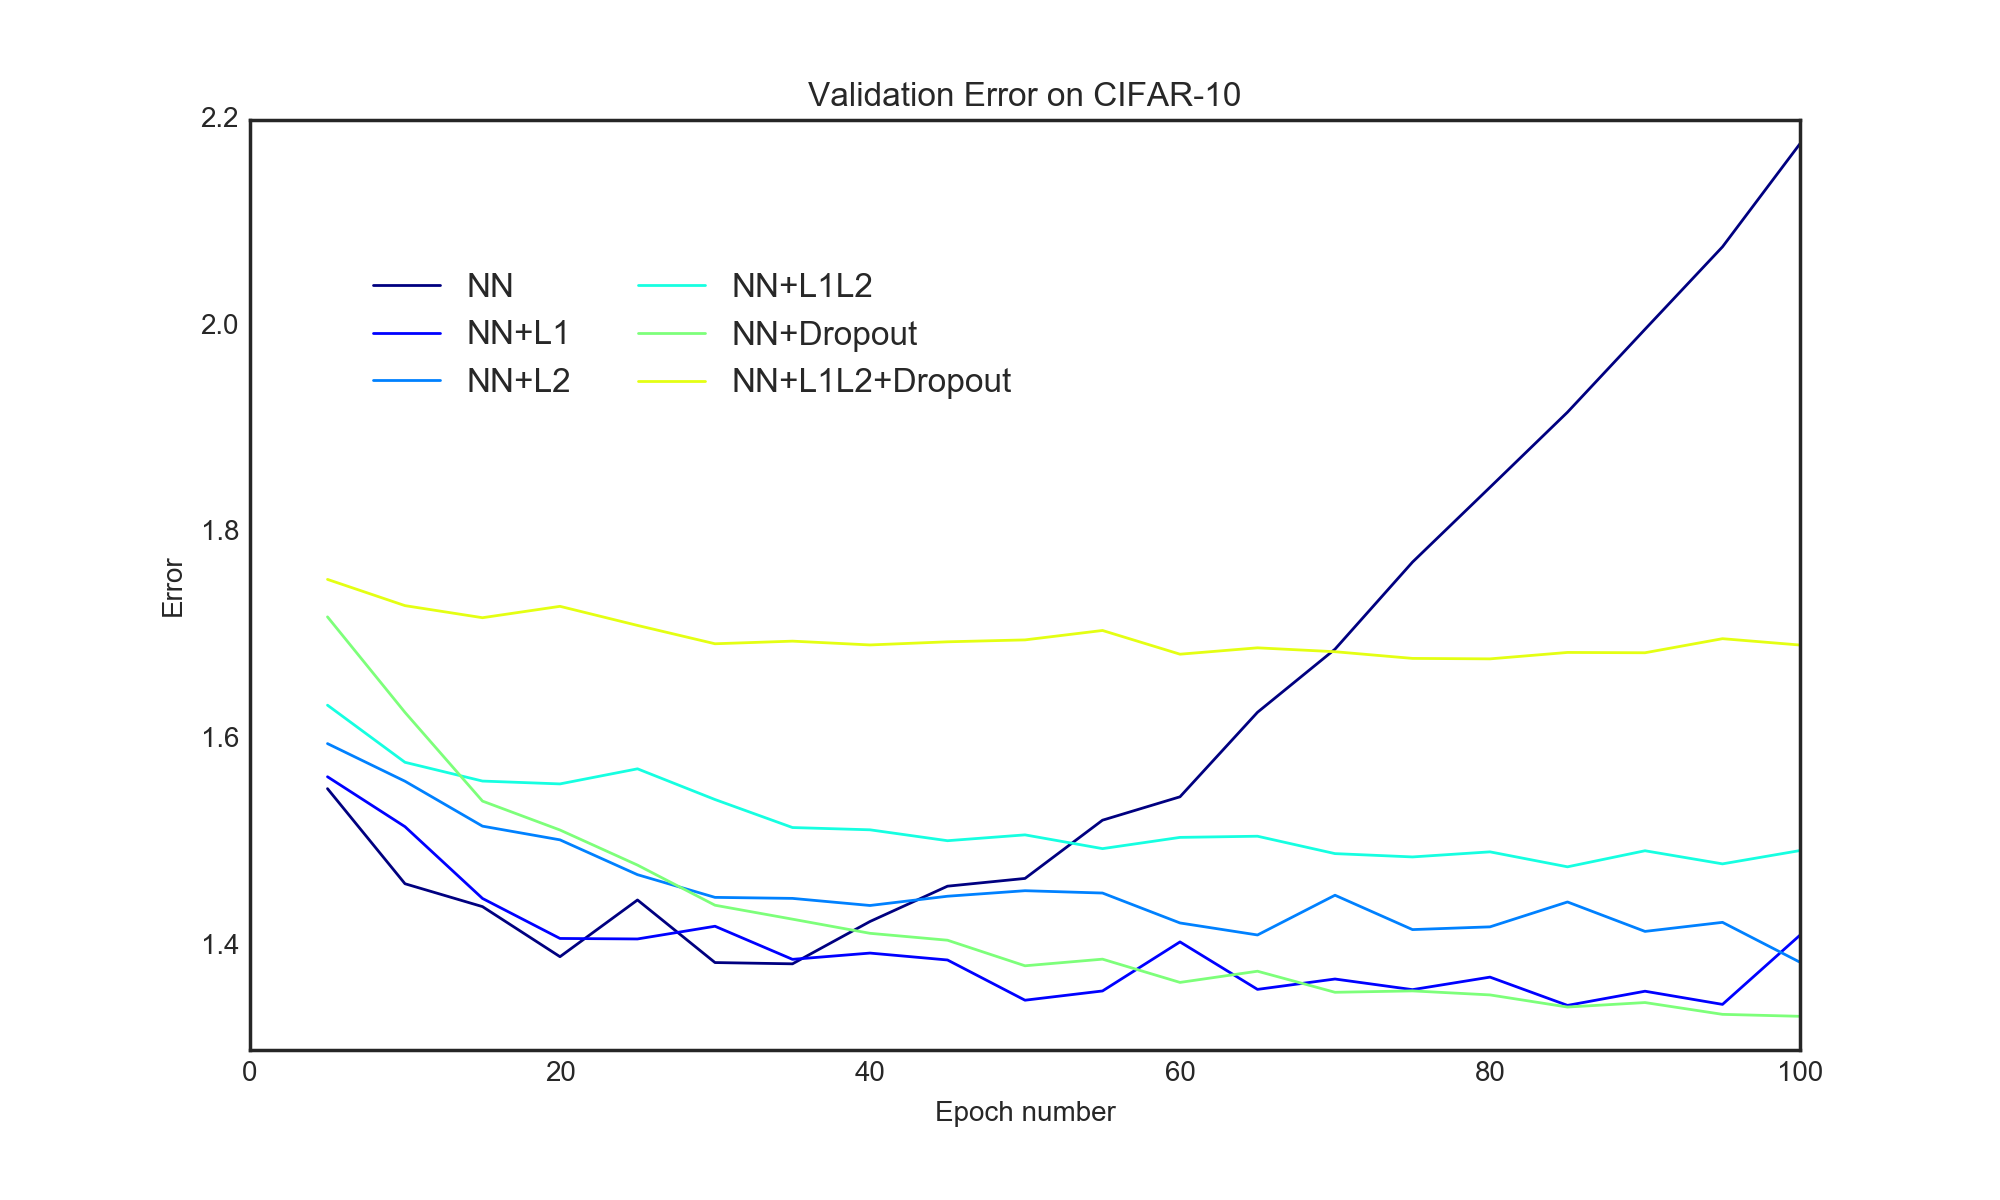
\includegraphics[width=3in]{Regularisation_valid_err_2}
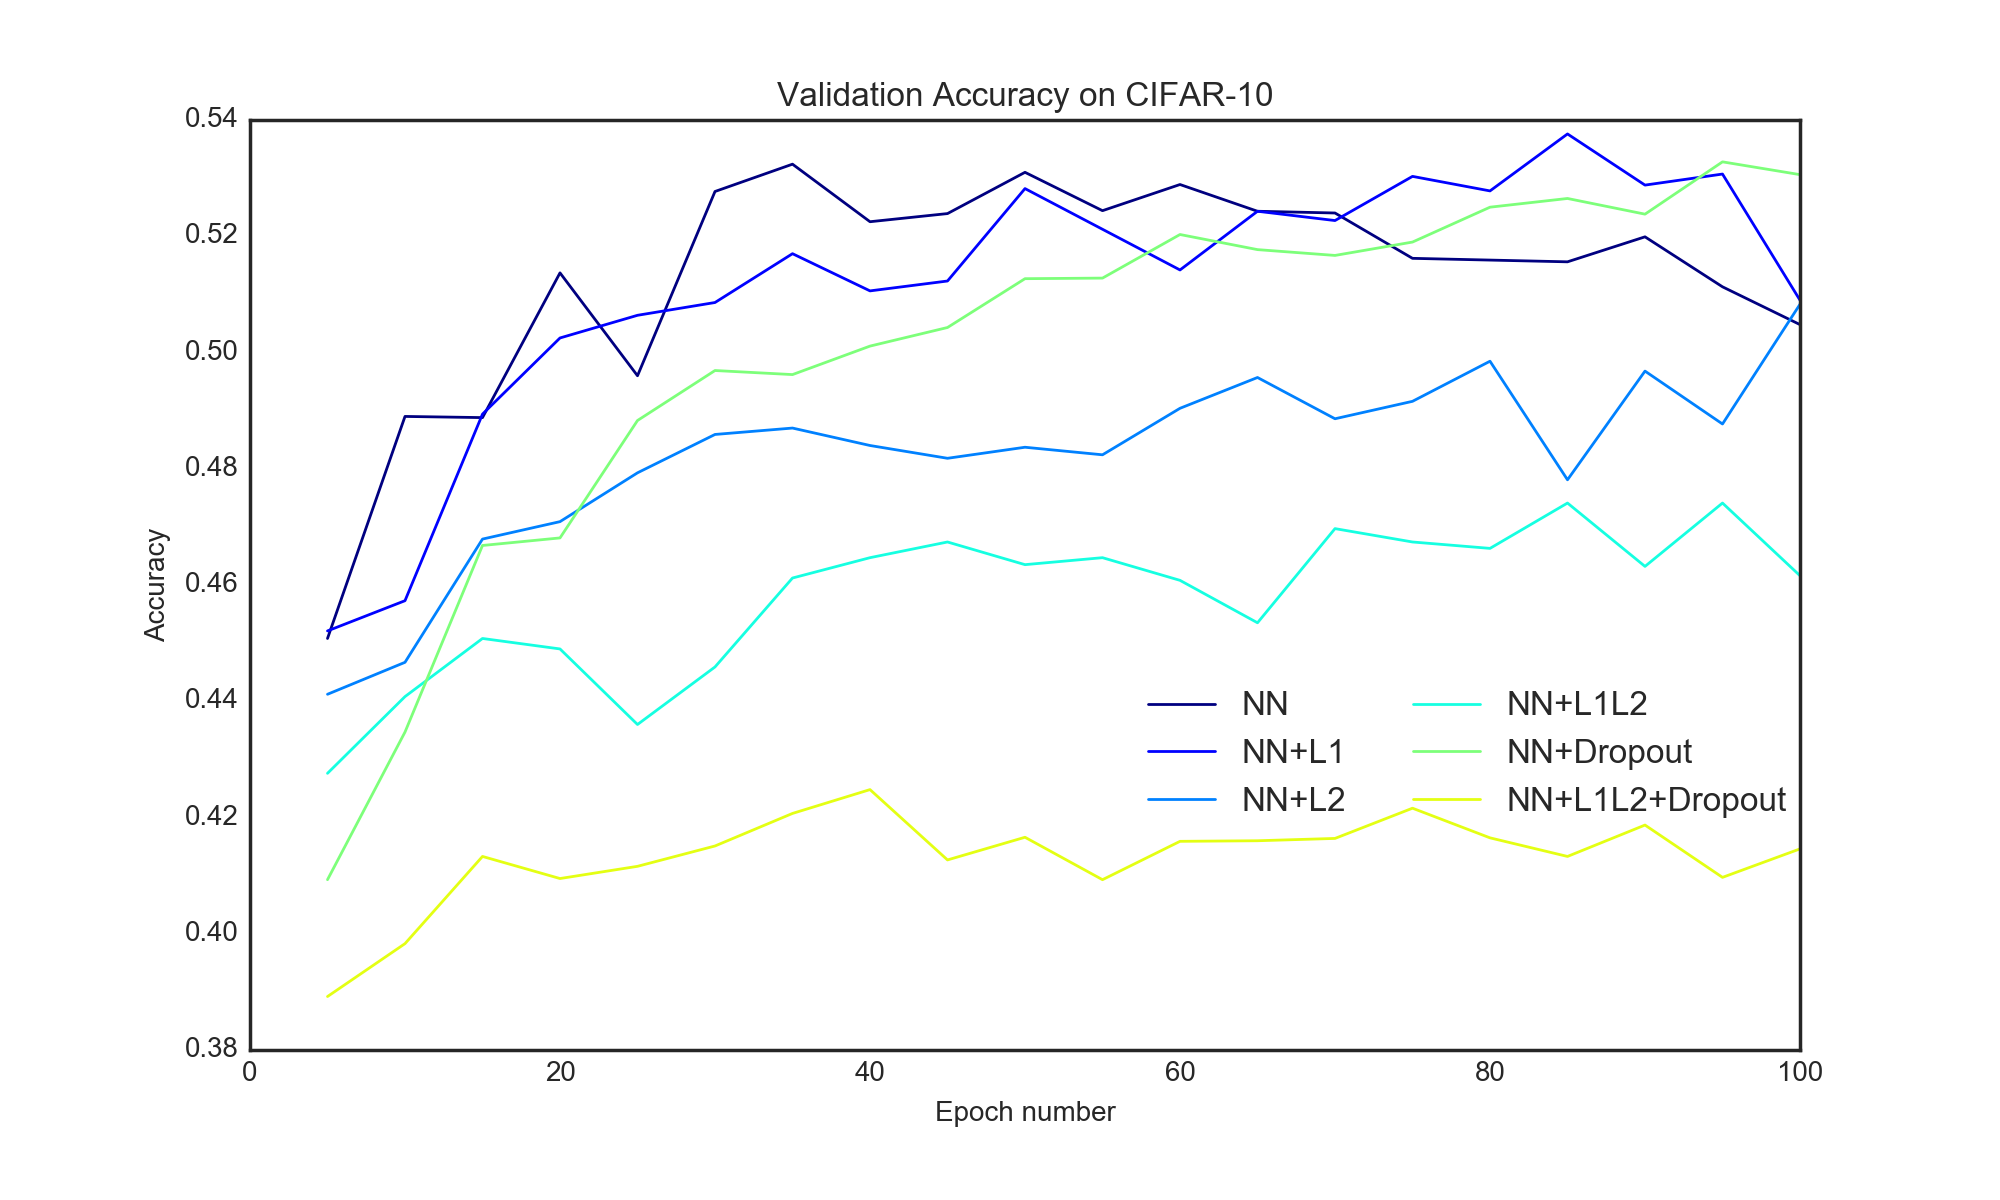
\includegraphics[width=3in]{Regularisation_valid_acc_2}

The evolution plots(of CIFAR-10) are shown above.Since we have done a lot of experiments of L1 and L2 regularisation in previous coursework, we will focus on dropout this time. From the plots, we could easily find that all these methods could effectively slowdown the training process and prevent over-fitting. Also, we could indicate that dropout approach gives the best result(it has lowest error value) among the experiments. Dropout considerably improves the performance of standard neural networks. For further evaluation, we also calculate the average training time of each method. 
\begin{table}[!ht]
\centering 
\caption{Experiment Design for L1 \& L2 Regularisation and Dropout}
\begin{tabular}{c c}
\toprule
No. & Average training time of each epoch(s) \\
\midrule
1 & 12.10\\
2 & 26.08\\
3 & 16.49\\
4 & 26.64\\
5 & 15.95\\
6 & 27.44\\
\bottomrule
\end{tabular}
\end{table}

From the table 5, it is strange that dropout method will cost more time than normal neural network(compare experiment 1 and 5) although it only trains less units of network. According to Srivastava(2014), a major answer to this phenomenon is that the parameter updates are very noisy. Each training case effectively tries to train a different random architecture. Therefore, the gradients that are being computed are not the gradients of the final architecture that will be used at test time. Despite this, dropout is also worth a trying in future work on CIFAR-100 because it has been proved to be able to improve the performance of convolutional networks.

For more training results on CIFAR-100, please see appendix in the end of the report.
\section{Future Work}

In this experiments, we have tried different NN architectures, different activation functions, normalisation and regularisation on feed-forward networks. All these works have reference value for further experiments.

According to He's(2015) work, deep residual network could generate very good results on both CIFAR-10 and CIFAR-100 datasets. We could also follow their experiments to have a try on complex neural networks.

For the first step, we need to implement convolutional network and do some related experiments with it. Since we only have a cluster of CPUs, we could build some small CNN to evaluate the accuracy.

Secondly, following He's work, we could apply residual learning part to our trained CNN. As this will cost a lot of time, we need to do it earlier.

Finally, by applying the techniques we used in this experiment, we could optimize our model to see if we could get improved results.
\newpage
\section{Reference}

Glorot, Xavier, and Yoshua Bengio. "Understanding the difficulty of training deep feedforward neural networks." Aistats. Vol. 9. 2010.

He, Kaiming, et al. "Deep residual learning for image recognition." Proceedings of the IEEE Conference on Computer Vision and Pattern Recognition. 2016.

Ba, Jimmy, and Rich Caruana. "Do deep nets really need to be deep?." Advances in neural information processing systems. 2014.

LeCun, Yann, Yoshua Bengio, and Geoffrey Hinton. "Deep learning." Nature 521.7553 (2015): 436-444.

Michael Nielsen, Neural Networks and Deep Learning, 2015.

Srivastava, Nitish, et al. "Dropout: a simple way to prevent neural networks from overfitting." Journal of Machine Learning Research 15.1 (2014): 1929-1958.

Ioffe, Sergey, and Christian Szegedy. "Batch normalization: Accelerating deep network training by reducing internal covariate shift." arXiv preprint arXiv:1502.03167 (2015).

Xu, Bing, et al. "Empirical evaluation of rectified activations in convolutional network." arXiv preprint arXiv:1505.00853 (2015).

\newpage
\section{Appendix}
\subsection{Evolution plots of network architectures experiments on CIFAR-100}
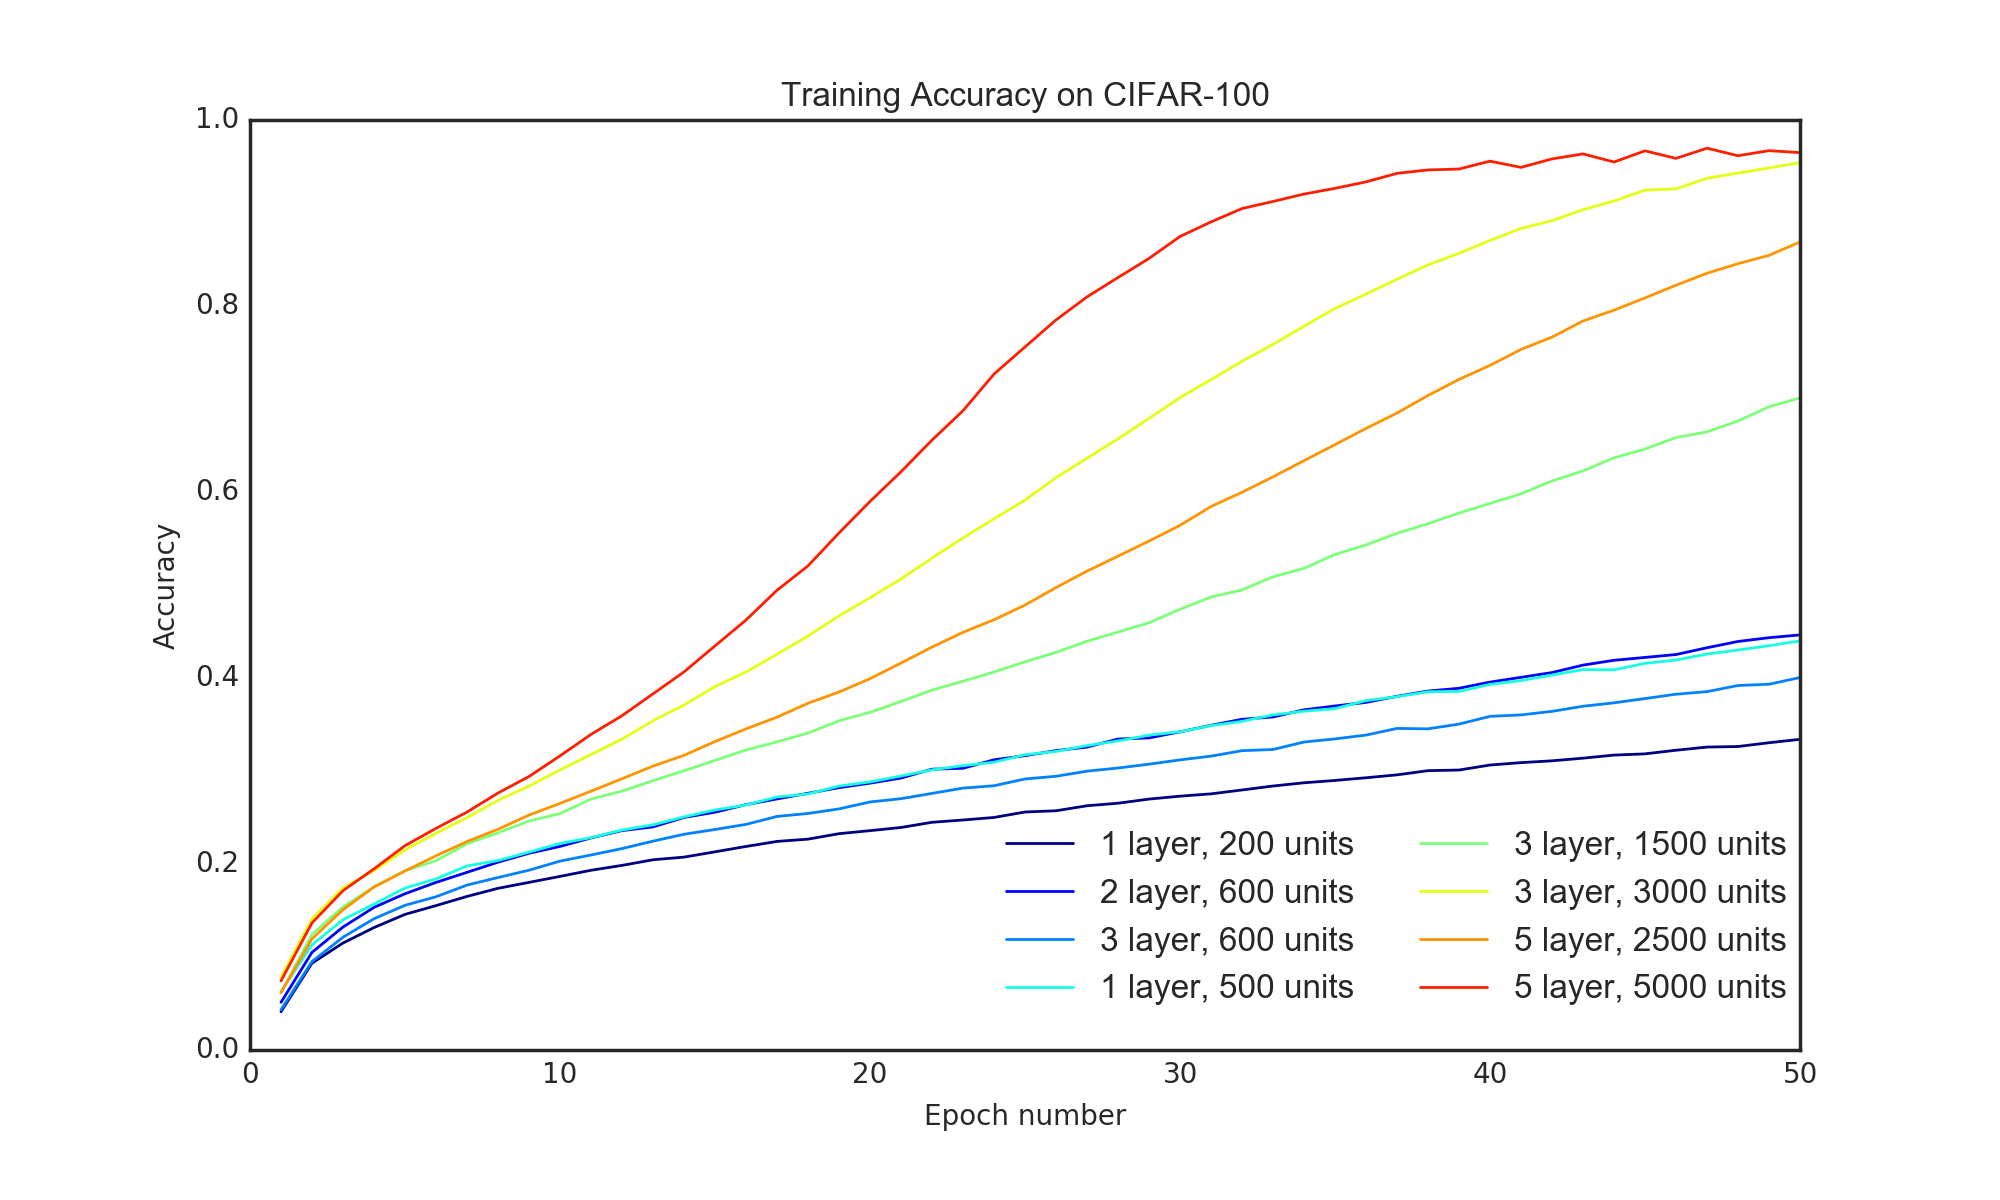
\includegraphics[width=3in]{NN_architures_train_acc_100}
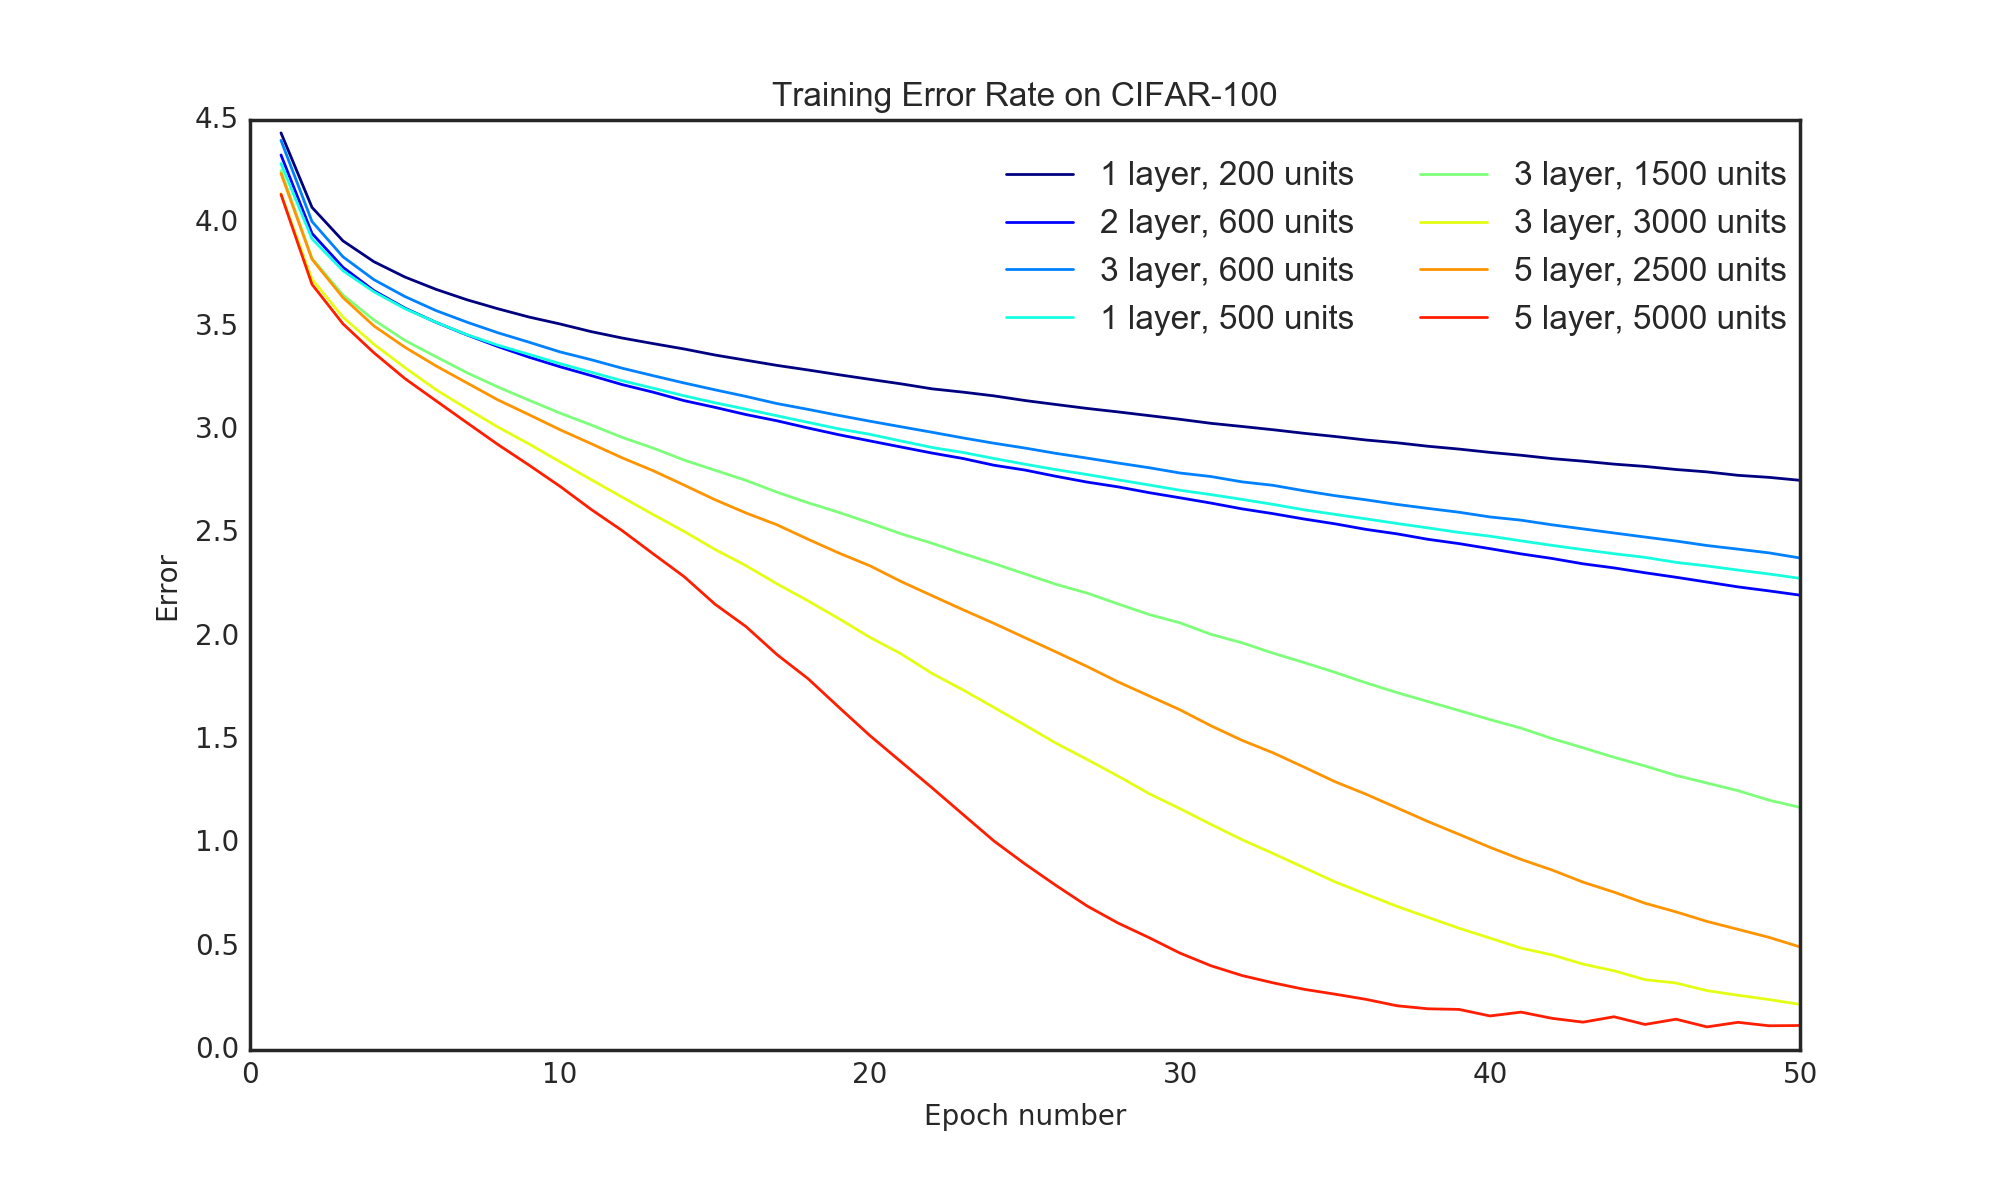
\includegraphics[width=3in]{NN_architures_train_err_100}

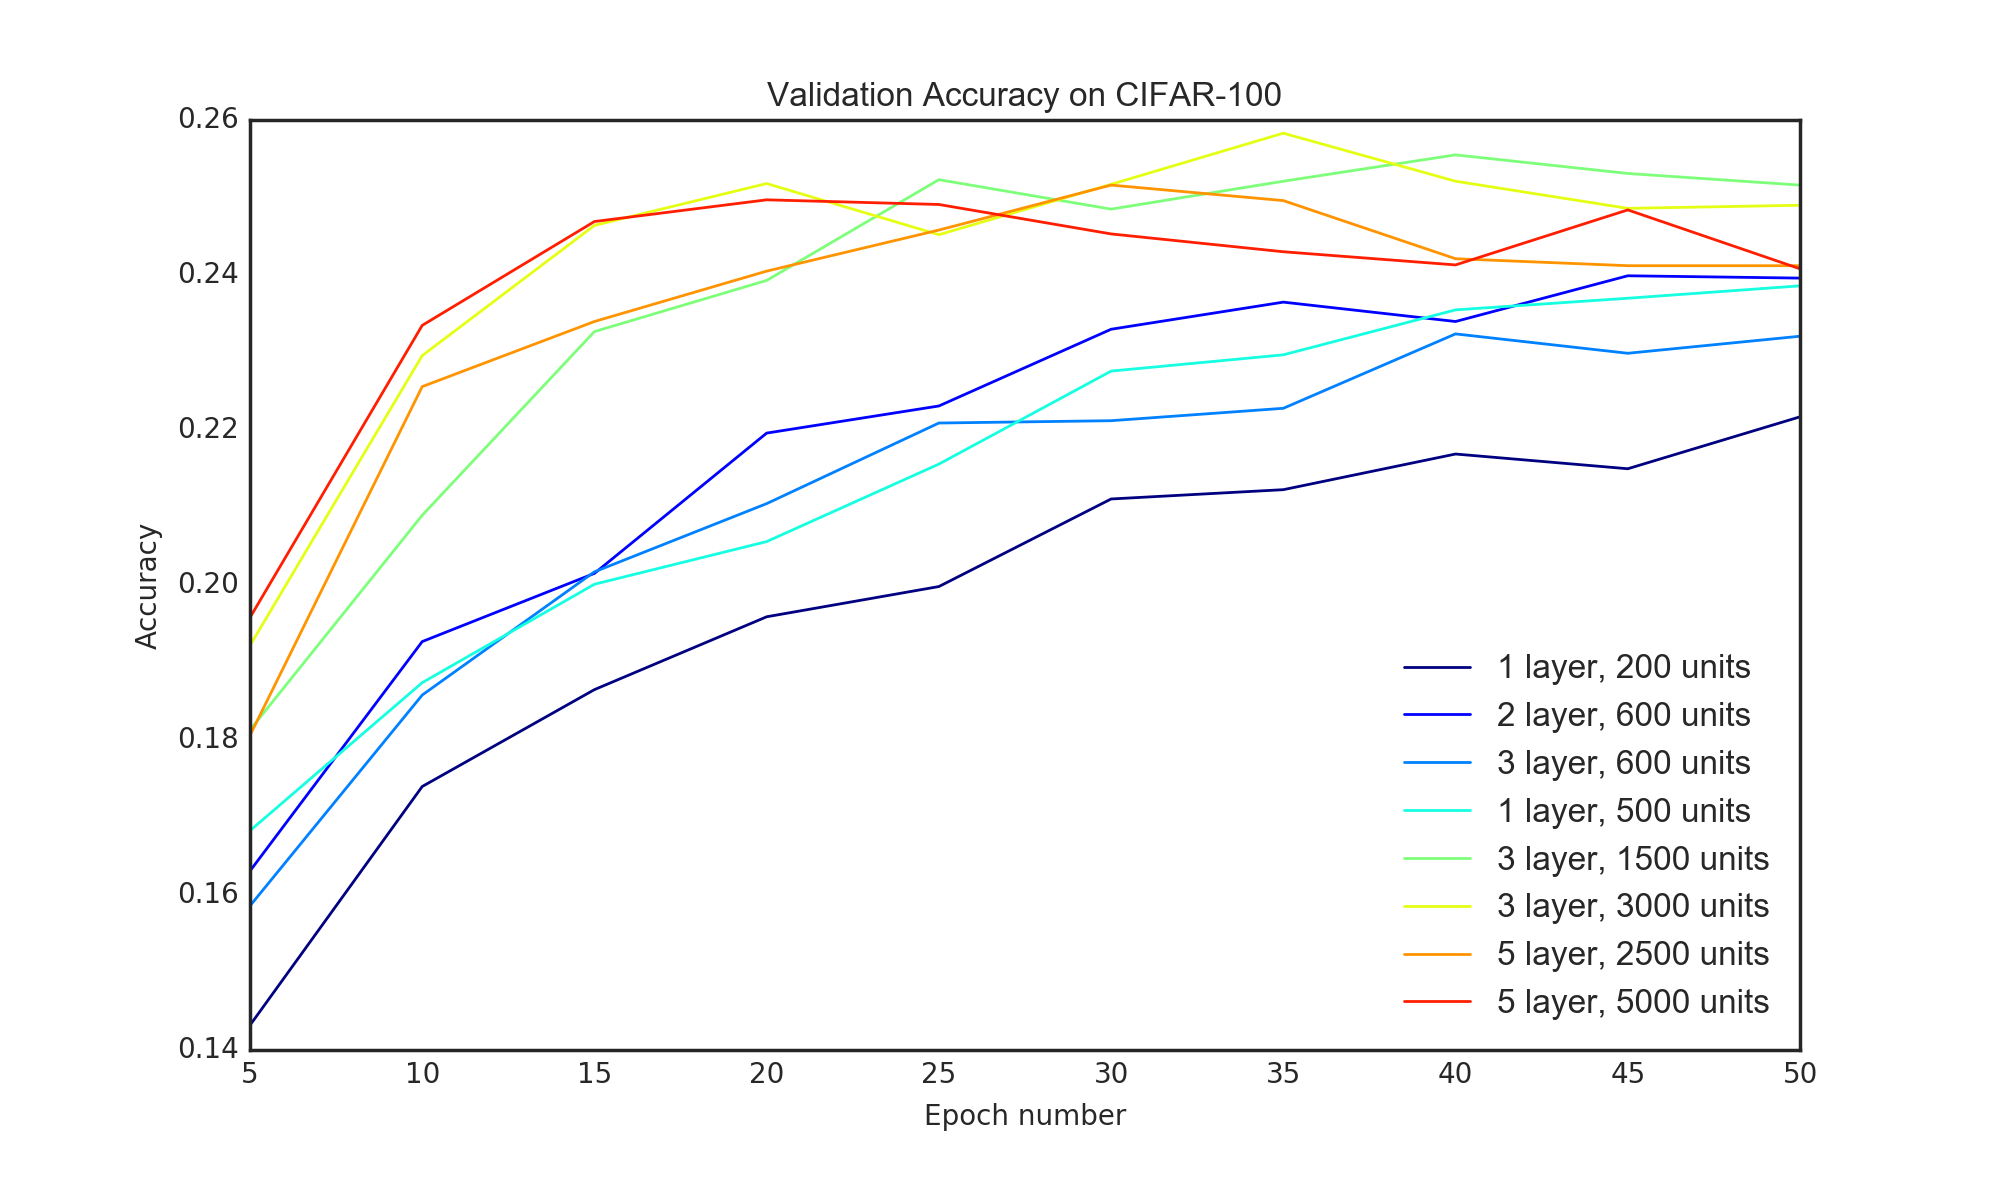
\includegraphics[width=3in]{NN_architures_valid_acc_100}
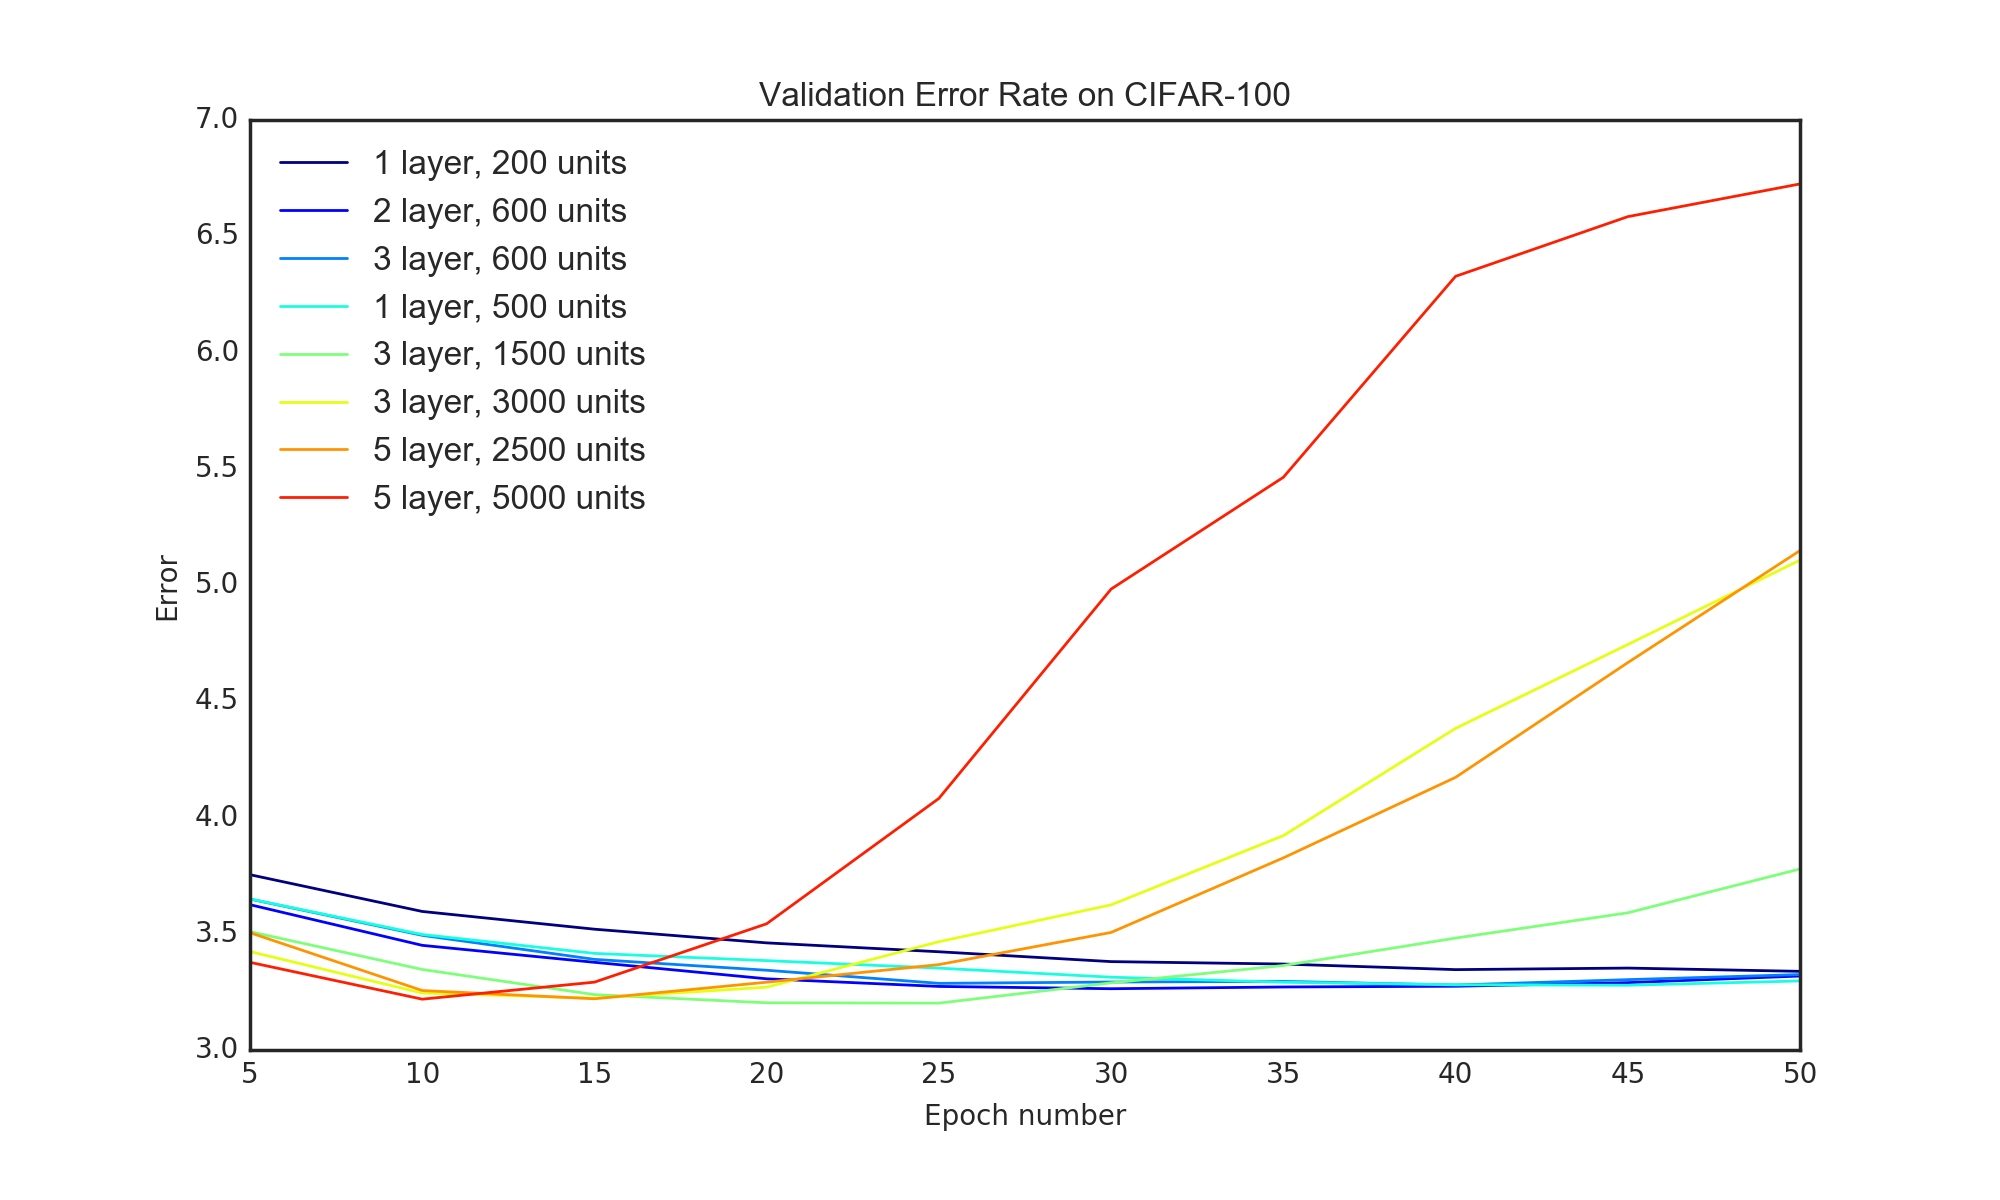
\includegraphics[width=3in]{NN_architures_valid_err_100}

\subsection{Evolution plots of batch normalisation on CIFAR-100}
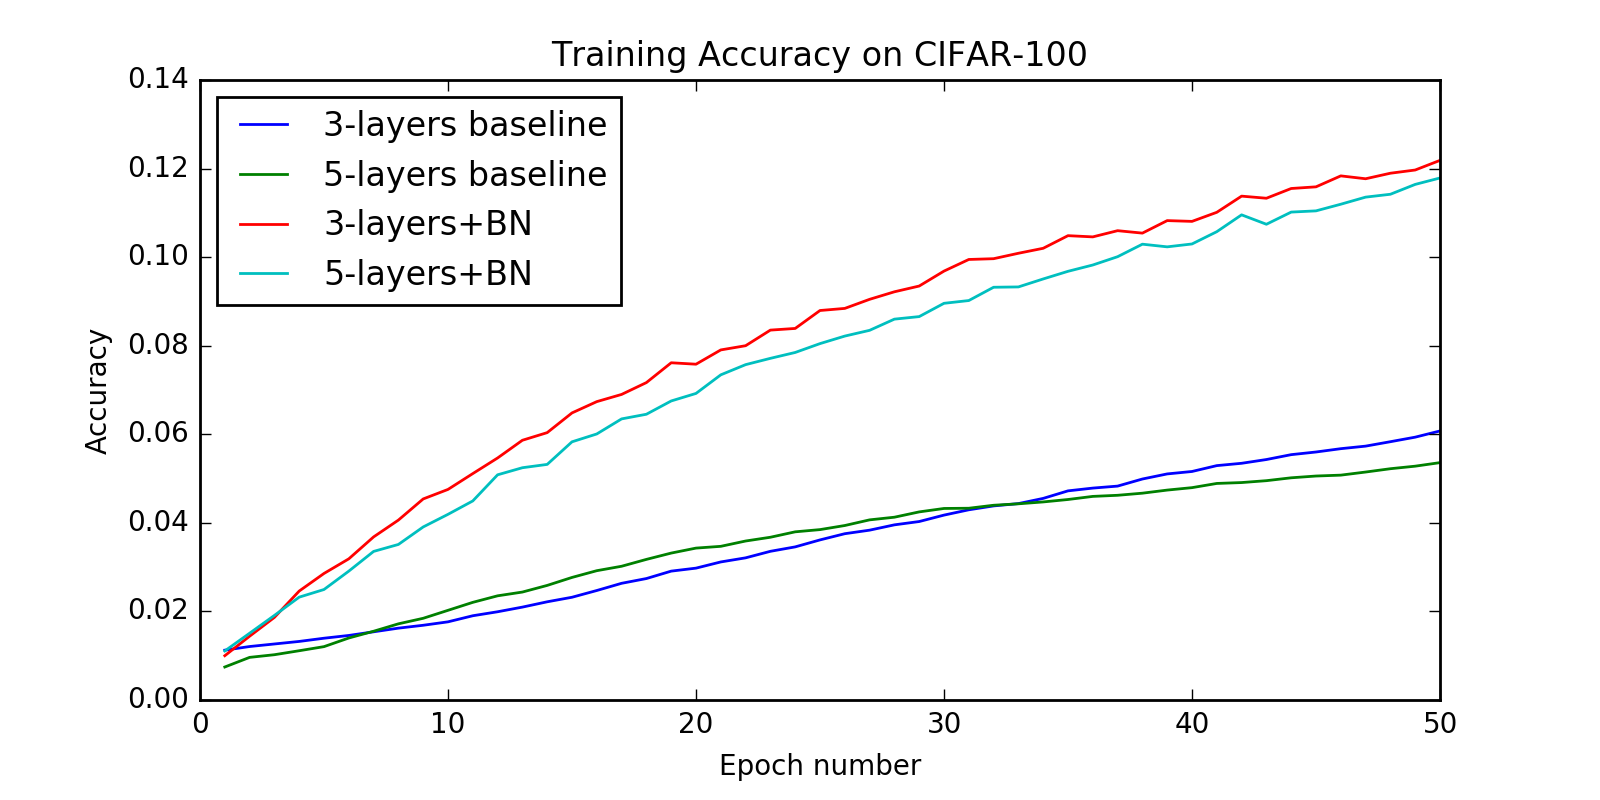
\includegraphics[width=3in]{BN_train_acc_100}
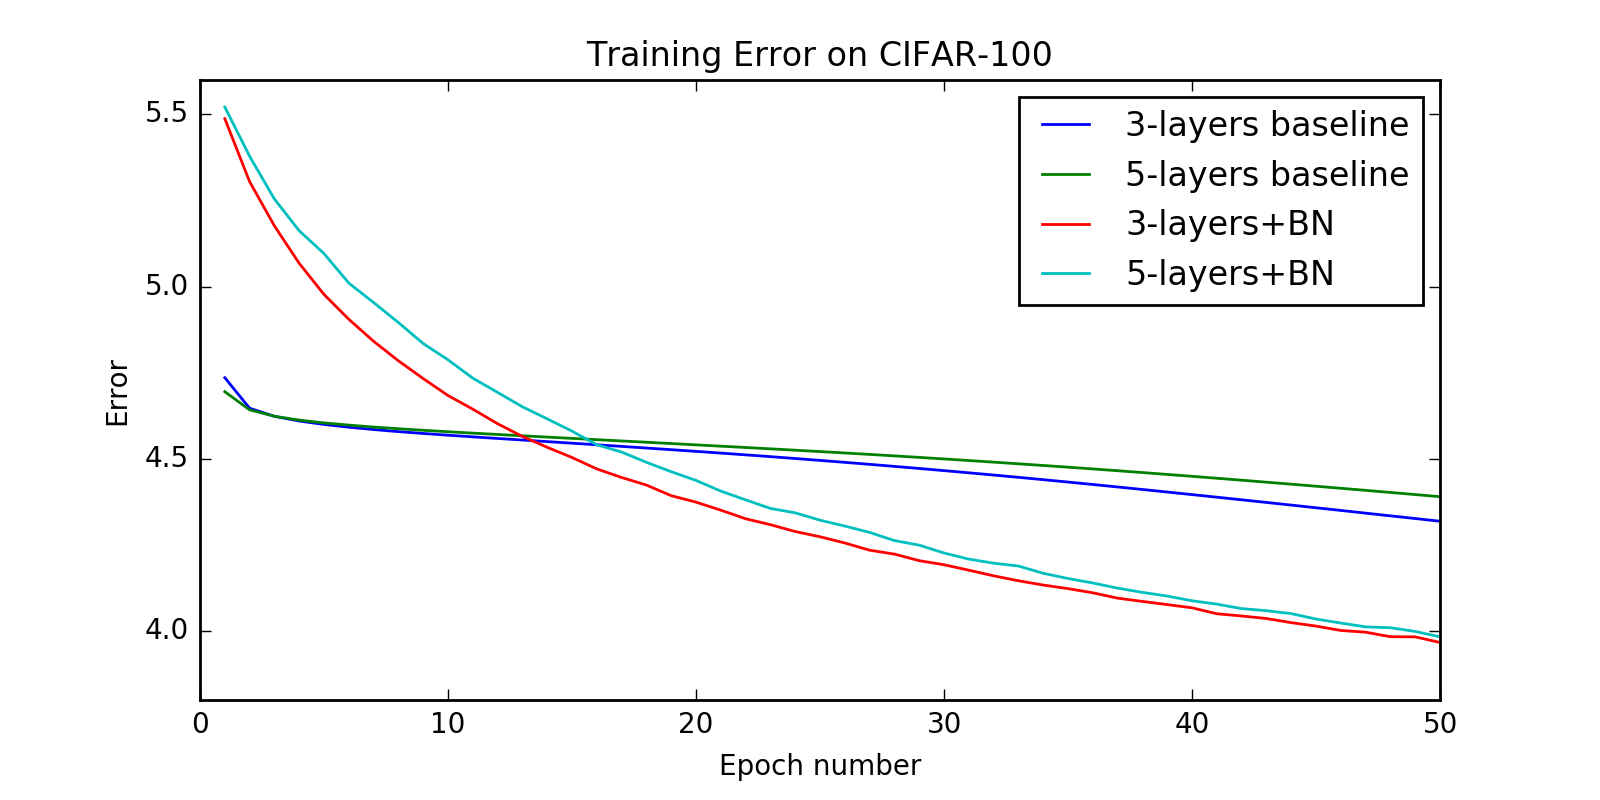
\includegraphics[width=3in]{BN_train_err_100}

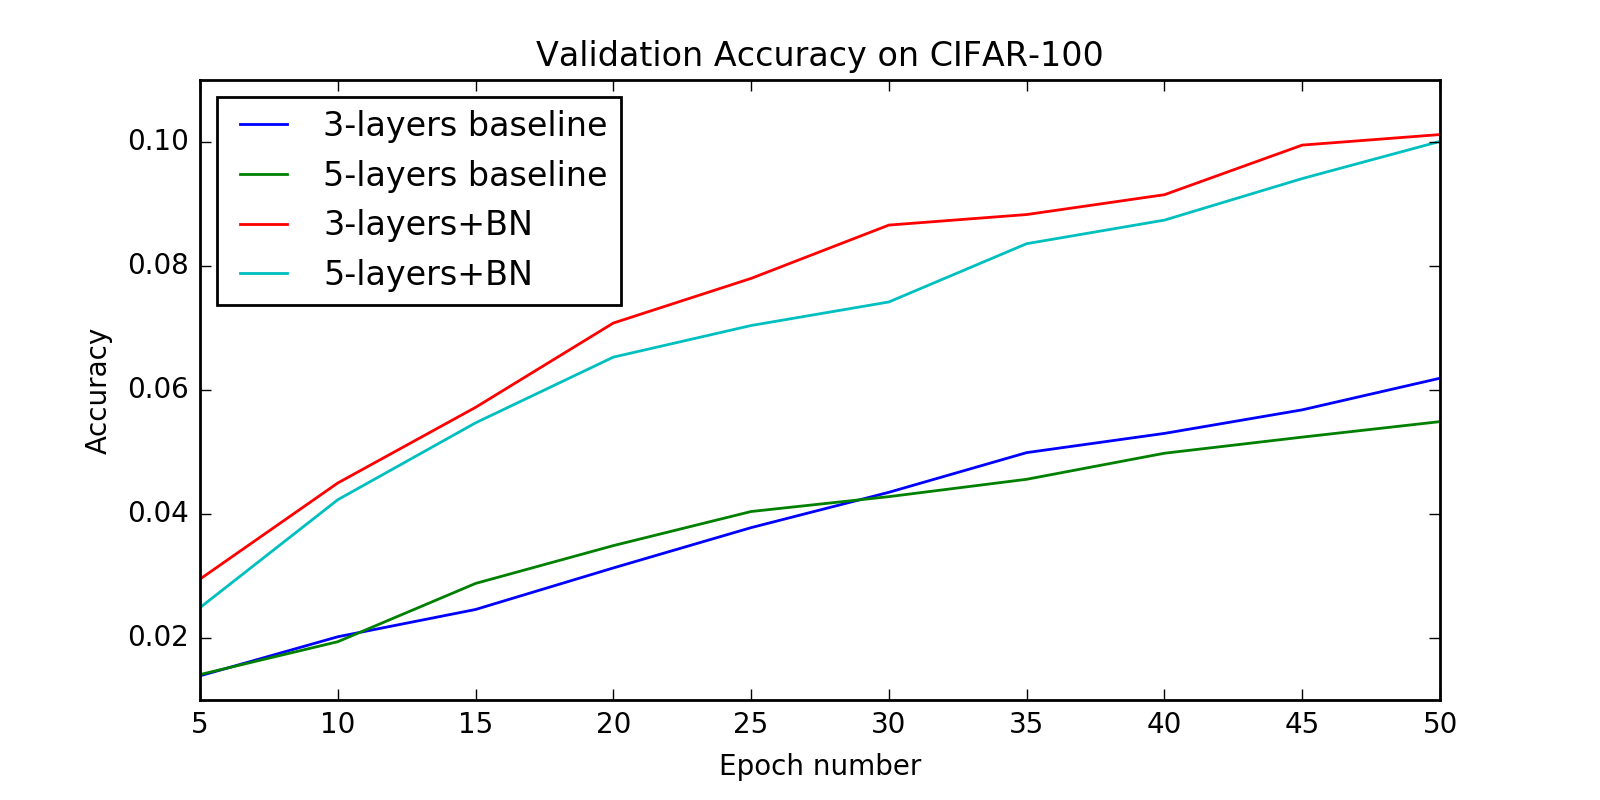
\includegraphics[width=3in]{BN_valid_acc_100}
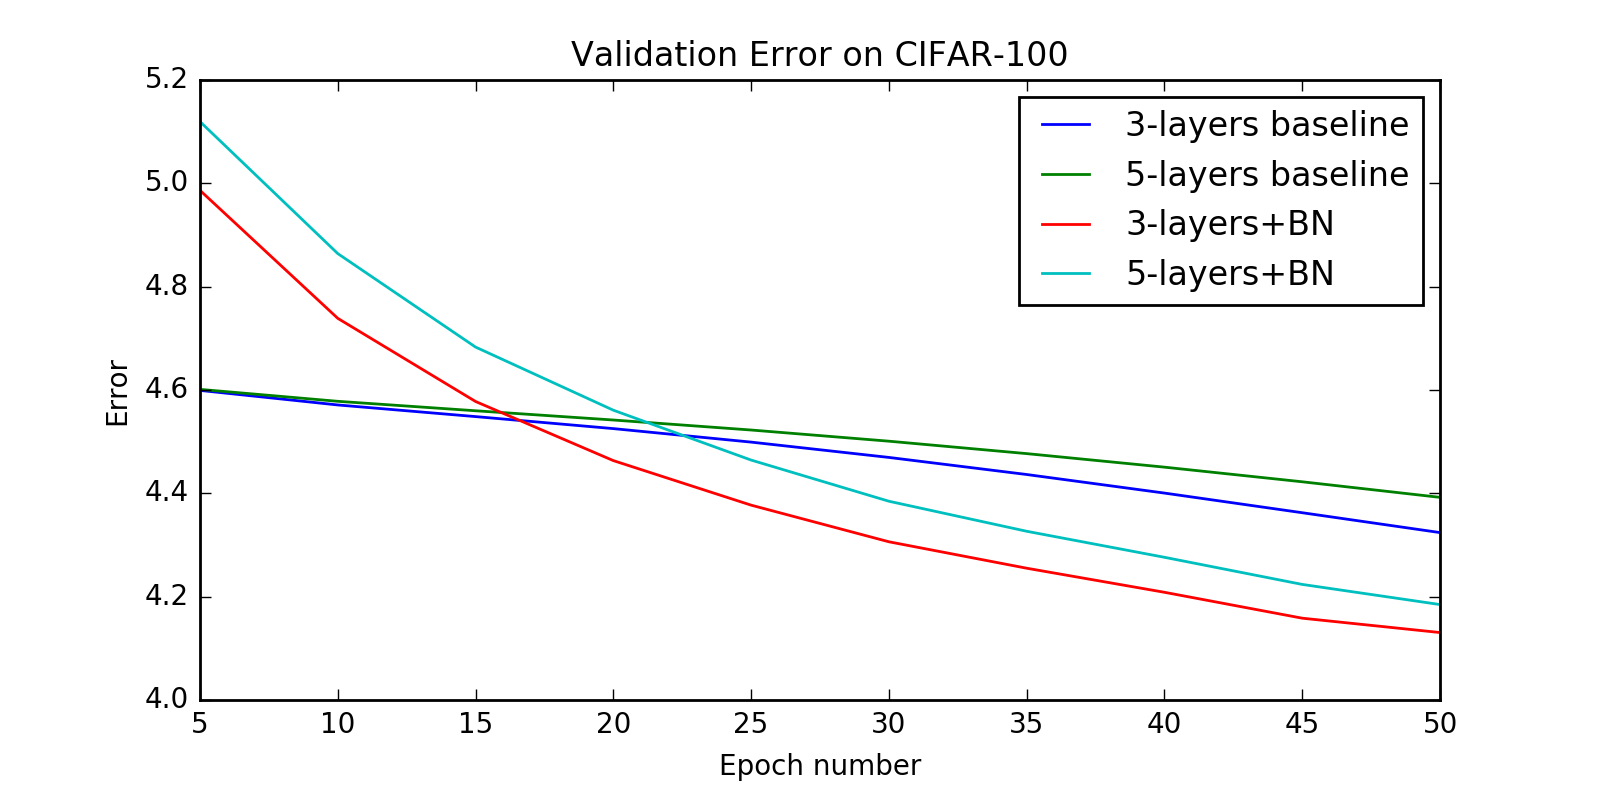
\includegraphics[width=3in]{BN_valid_err_100}

\subsection{Evolution plots of regularisation experiments on CIFAR-100}
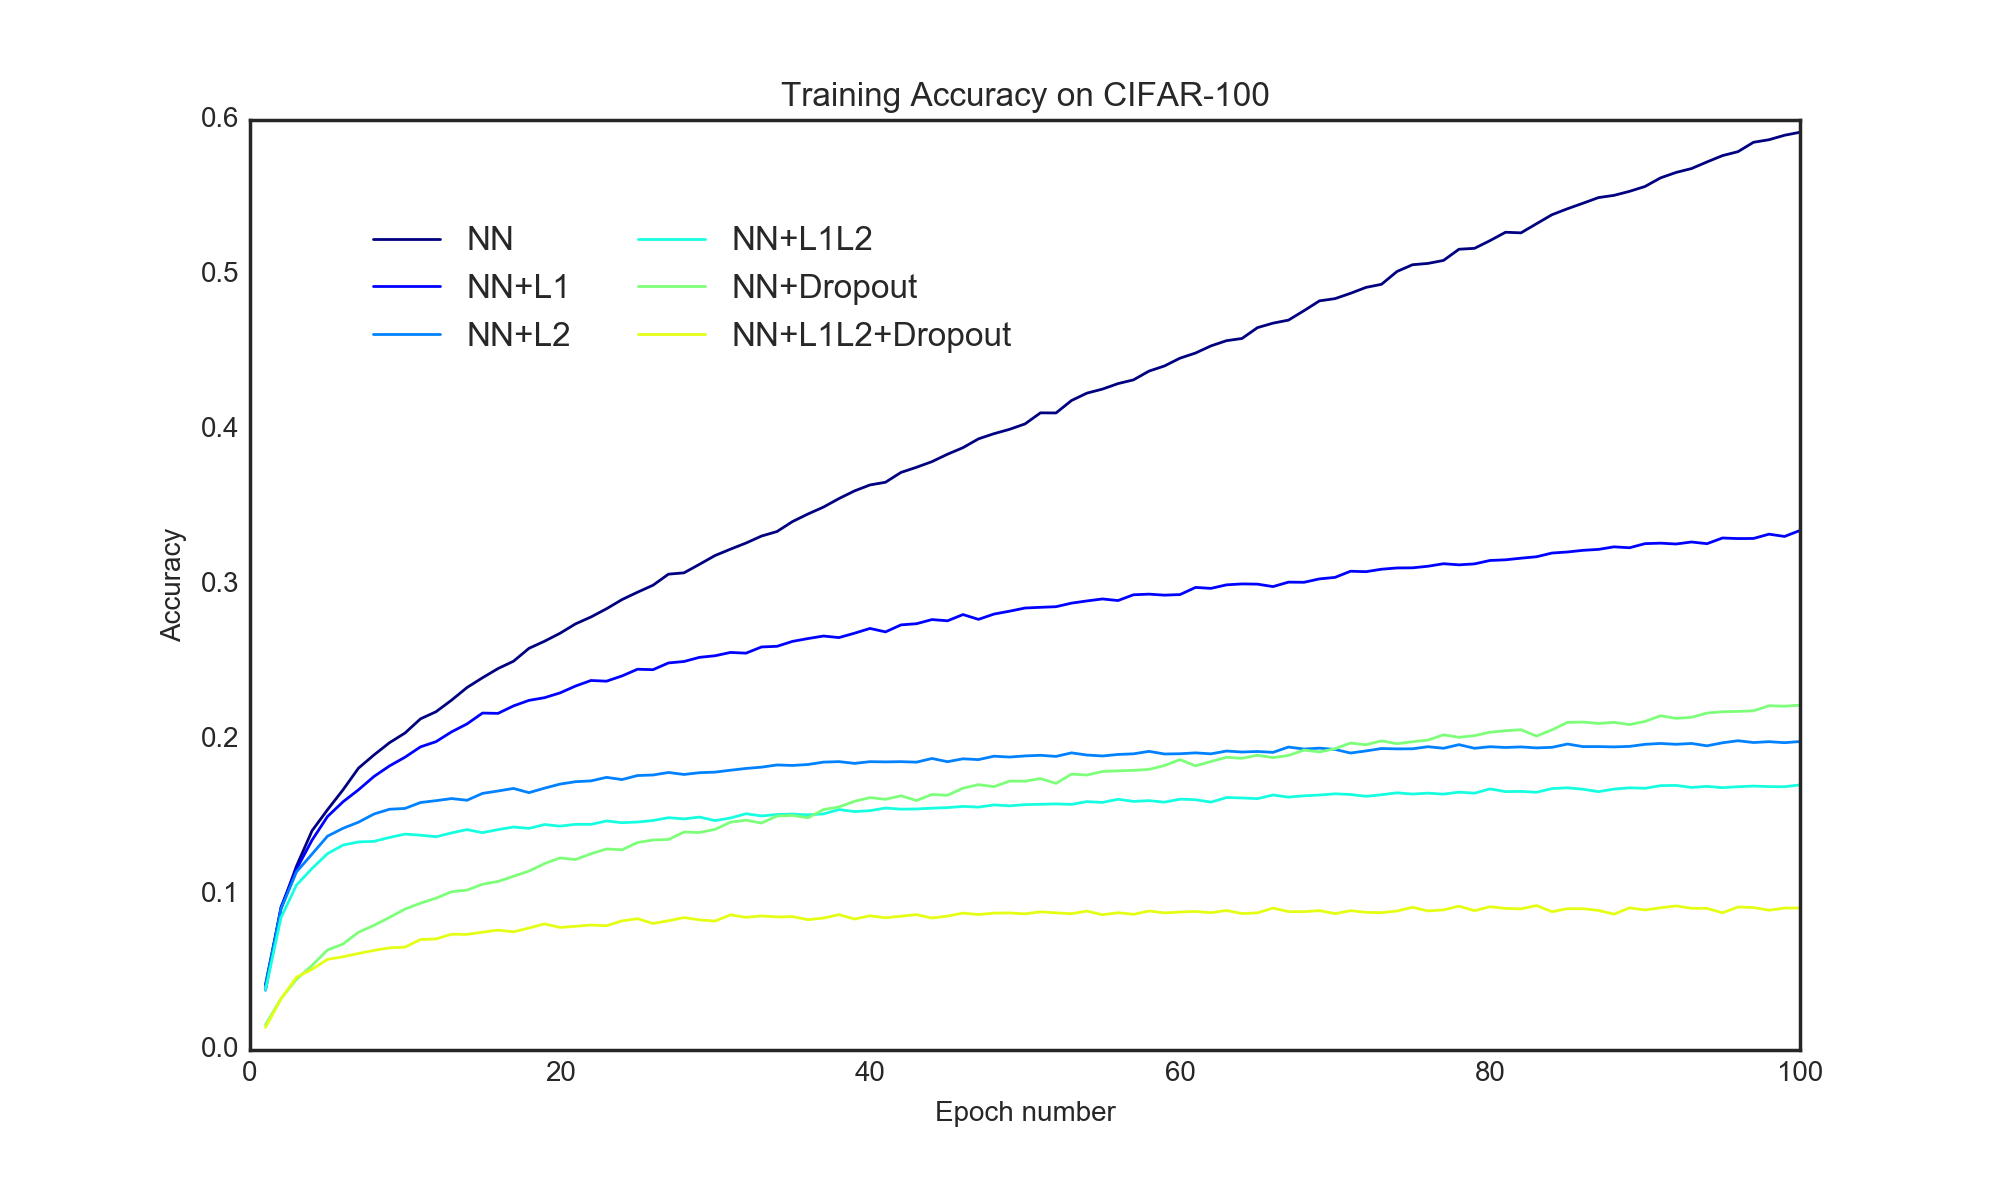
\includegraphics[width=3in]{Regularisation_train_acc_100}
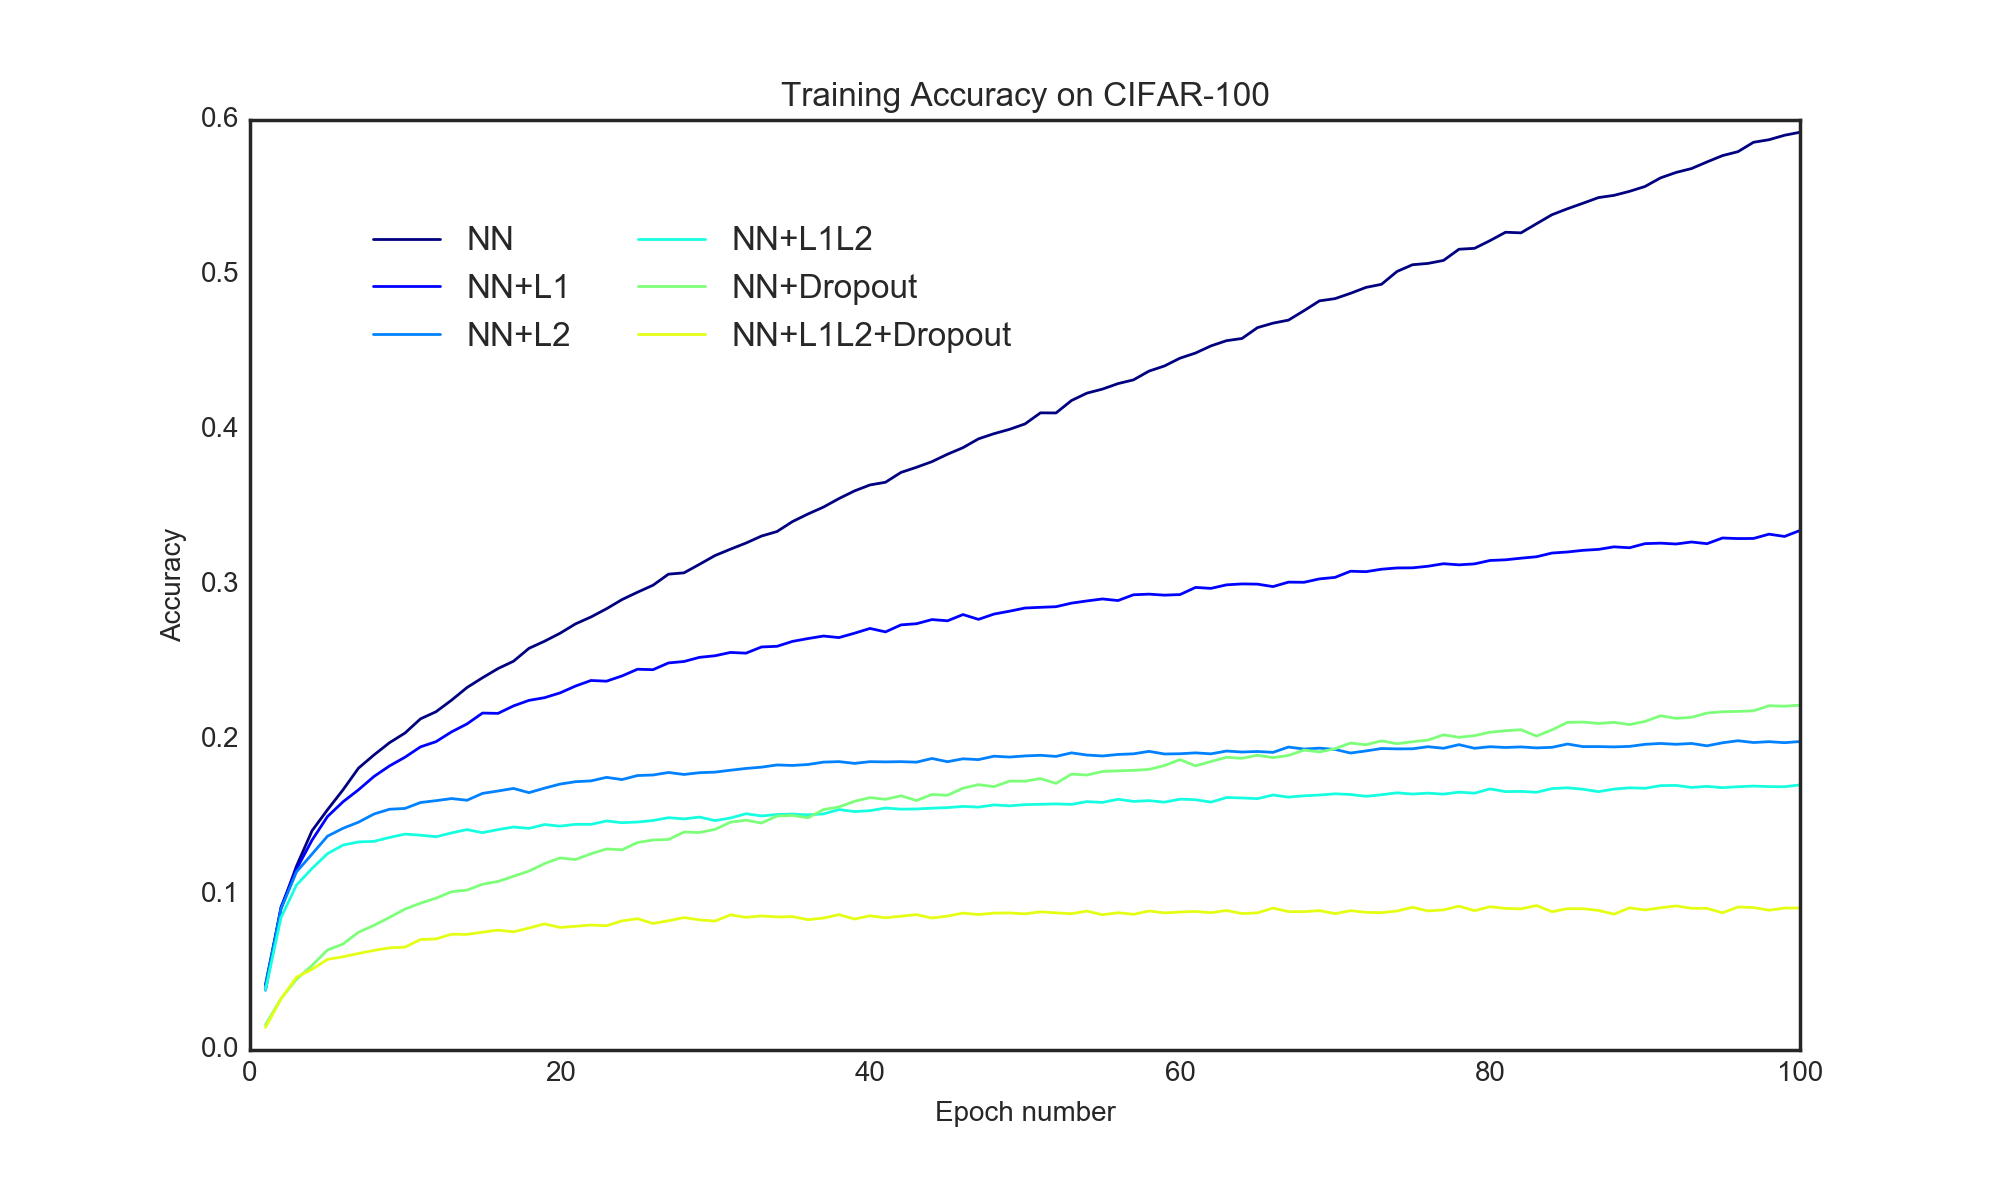
\includegraphics[width=3in]{Regularisation_train_acc_100}

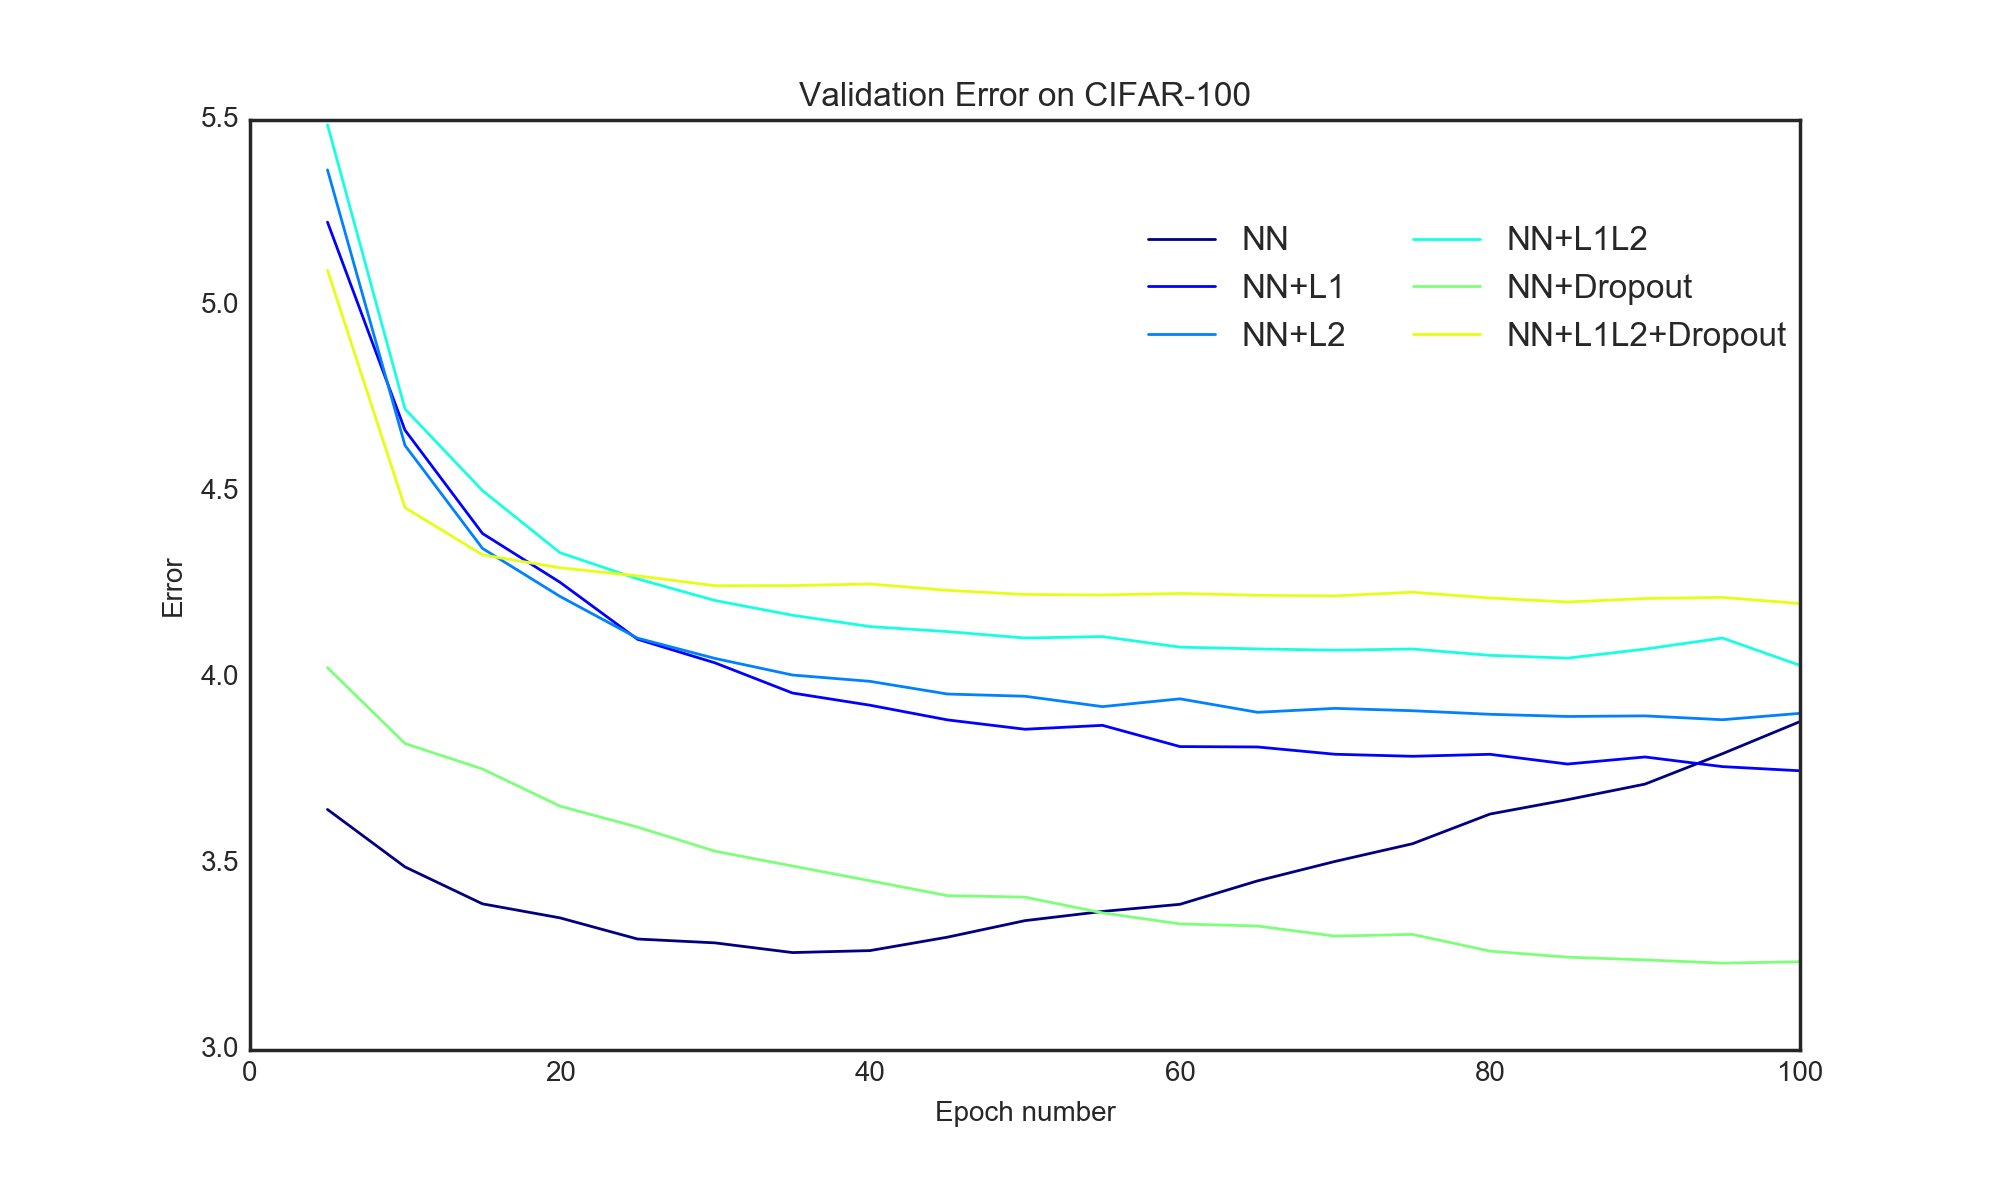
\includegraphics[width=3in]{Regularisation_valid_err_100}
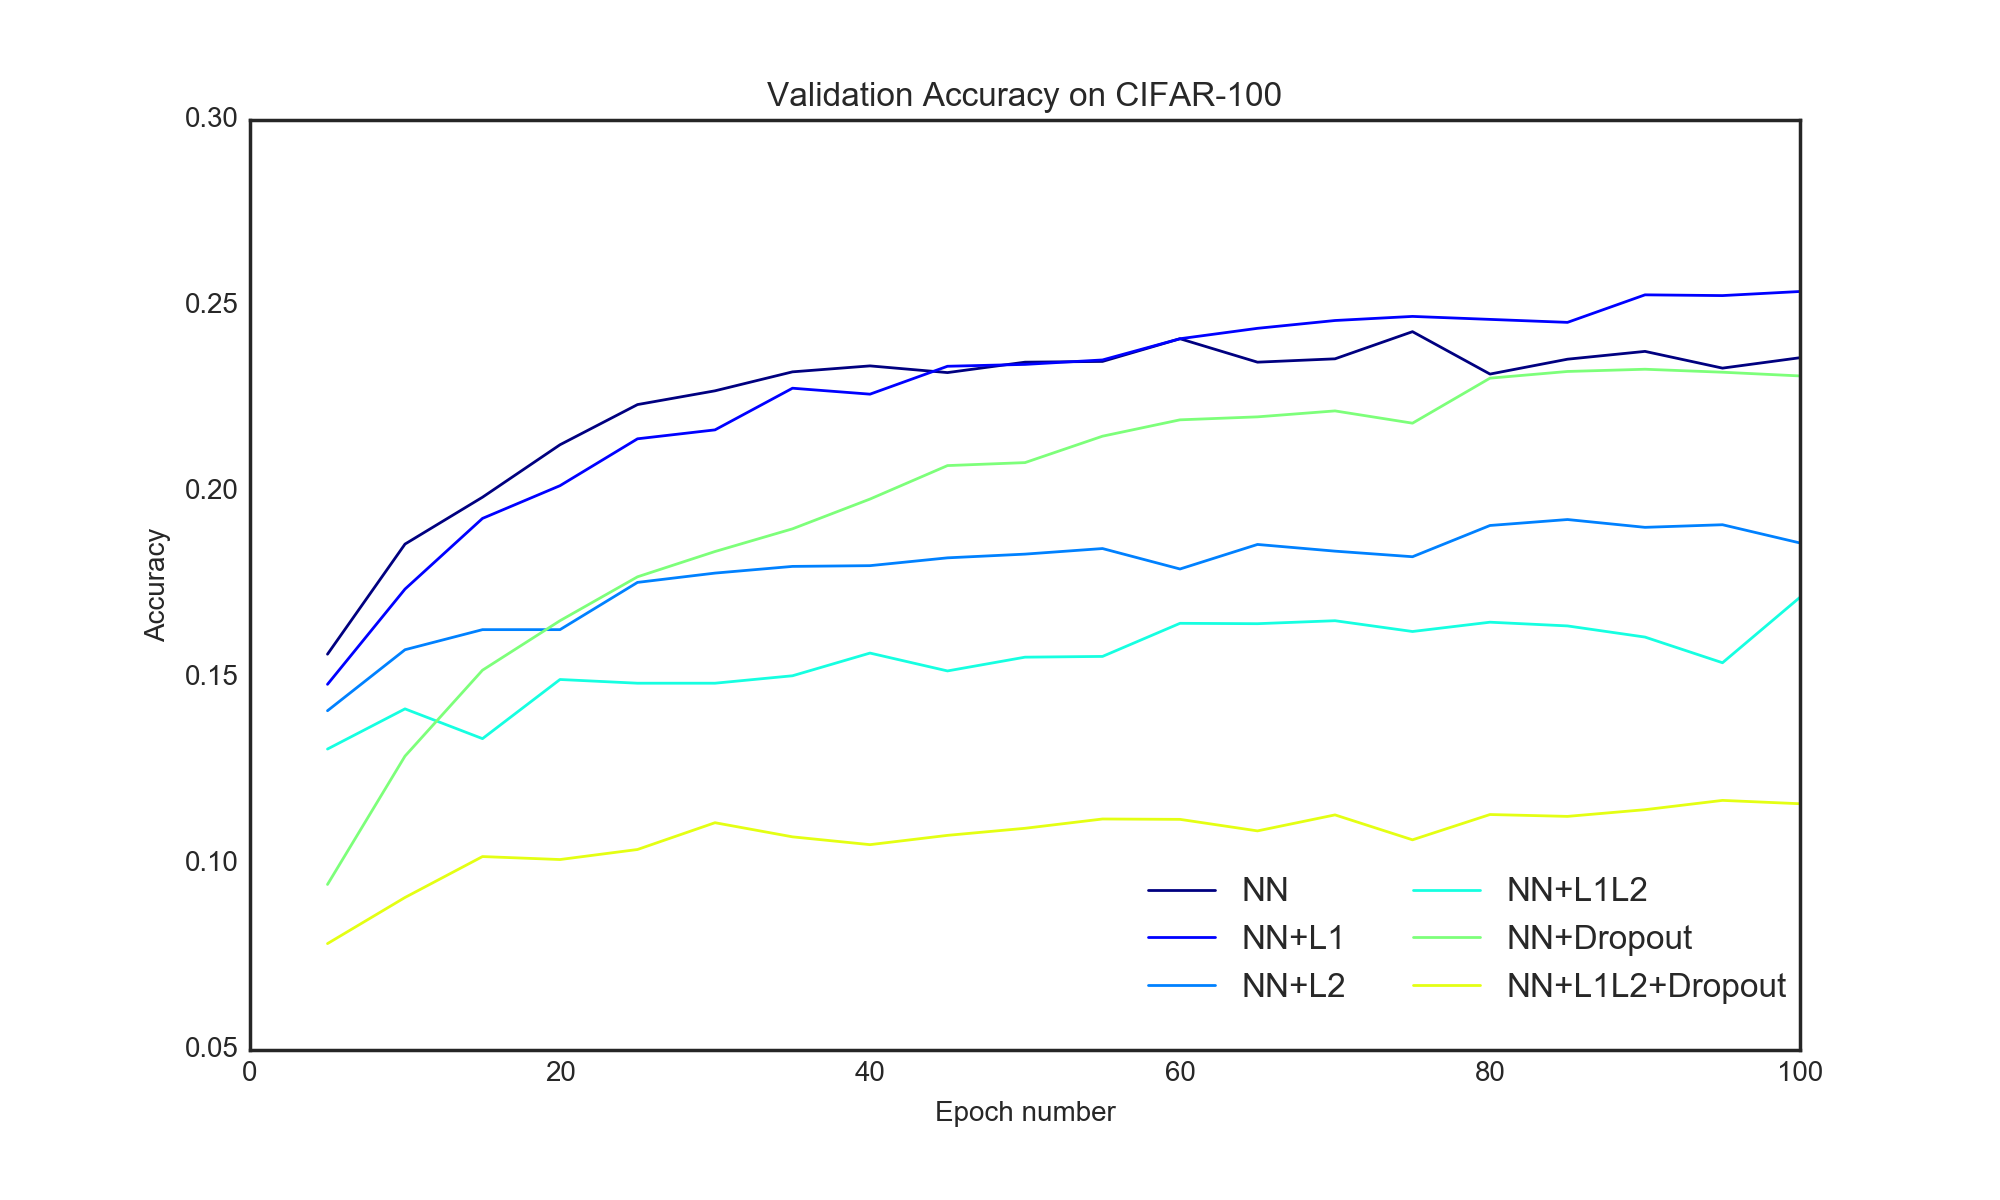
\includegraphics[width=3in]{Regularisation_valid_acc_100}

\end{document}
